% Template for PLoS
% Version 3.4 January 2017
%
% % % % % % % % % % % % % % % % % % % % % %
%
% -- IMPORTANT NOTE
%
% This template contains comments intended
% to minimize problems and delays during our production
% process. Please follow the template instructions
% whenever possible.
%
% % % % % % % % % % % % % % % % % % % % % % %
%
% Once your paper is accepted for publication,
% PLEASE REMOVE ALL TRACKED CHANGES in this file
% and leave only the final text of your manuscript.
% PLOS recommends the use of latexdiff to track changes during review, as this will help to maintain a clean tex file.
% Visit https://www.ctan.org/pkg/latexdiff?lang=en for info or contact us at latex@plos.org.
%
%
% There are no restrictions on package use within the LaTeX files except that
% no packages listed in the template may be deleted.
%
% Please do not include colors or graphics in the text.
%
% The manuscript LaTeX source should be contained within a single file (do not use \input, \externaldocument, or similar commands).
%
% % % % % % % % % % % % % % % % % % % % % % %
%
% -- FIGURES AND TABLES
%
% Please include tables/figure captions directly after the paragraph where they are first cited in the text.
%
% DO NOT INCLUDE GRAPHICS IN YOUR MANUSCRIPT
% - Figures should be uploaded separately from your manuscript file.
% - Figures generated using LaTeX should be extracted and removed from the PDF before submission.
% - Figures containing multiple panels/subfigures must be combined into one image file before submission.
% For figure citations, please use "Fig" instead of "Figure".
% See http://journals.plos.org/plosone/s/figures for PLOS figure guidelines.
%
% Tables should be cell-based and may not contain:
% - spacing/line breaks within cells to alter layout or alignment
% - do not nest tabular environments (no tabular environments within tabular environments)
% - no graphics or colored text (cell background color/shading OK)
% See http://journals.plos.org/plosone/s/tables for table guidelines.
%
% For tables that exceed the width of the text column, use the adjustwidth environment as illustrated in the example table in text below.
%
% % % % % % % % % % % % % % % % % % % % % % % %
%
% -- \texttt{EQU}ATIONS, MATH SYMBOLS, SUBSCRIPTS, AND SUPERSCRIPTS
%
% IMPORTANT
% Below are a few tips to help format your equations and other special characters according to our specifications. For more tips to help reduce the possibility of formatting errors during conversion, please see our LaTeX guidelines at http://journals.plos.org/plosone/s/latex
%
% For inline equations, please be sure to include all portions of an equation in the math environment.  For example, x$^2$ is incorrect; this should be formatted as $x^2$ (or $\mathrm{x}^2$ if the romanized font is desired).
%
% Do not include text that is not math in the math environment. For example, CO2 should be written as CO\textsubscript{2} instead of CO$_2$.
%
% Please add line breaks to long display equations when possible in order to fit size of the column.
%
% For inline equations, please do not include punctuation (commas, etc) within the math environment unless this is part of the equation.
%
% When adding superscript or subscripts outside of brackets/braces, please group using {}.  For example, change "[U(D,E,\gamma)]^2" to "{[U(D,E,\gamma)]}^2".
%
% Do not use \cal for caligraphic font.  Instead, use \mathcal{}
%
% % % % % % % % % % % % % % % % % % % % % % % %
%
% Please contact latex@plos.org with any questions.
%
% % % % % % % % % % % % % % % % % % % % % % % %

%make the document class option "10pt,letterpaper,final" to remove todo list items
\documentclass[10pt,letterpaper]{article}
\usepackage[top=0.85in,left=2.75in,footskip=0.75in]{geometry}

% amsmath and amssymb packages, useful for mathematical formulas and symbols
\usepackage{amsmath,amssymb}

% Use adjustwidth environment to exceed column width (see example table in text)
\usepackage{changepage}

% Use Unicode characters when possible
\usepackage[utf8x]{inputenc}

% textcomp package and marvosym package for additional characters
\usepackage{textcomp,marvosym}

% cite package, to clean up citations in the main text. Do not remove.
\usepackage{cite}

% Use nameref to cite supporting information files (see Supporting Information section for more info)
\usepackage{nameref,hyperref}

% line numbers
\usepackage[right]{lineno}

% ligatures disabled
\usepackage{microtype}
\DisableLigatures[f]{encoding = *, family = * }

% color can be used to apply background shading to table cells only
\usepackage[table]{xcolor}

% array package and thick rules for tables
\usepackage{array}

% additional packages
\usepackage{hhline}
\usepackage[obeyFinal,colorinlistoftodos]{todonotes}
\usepackage{courier}


% create "+" rule type for thick vertical lines
\newcolumntype{+}{!{\vrule width 2pt}}

% create \thickcline for thick horizontal lines of variable length
\newlength\savedwidth
\newcommand\thickcline[1]{%
  \noalign{\global\savedwidth\arrayrulewidth\global\arrayrulewidth 2pt}%
  \cline{#1}%
  \noalign{\vskip\arrayrulewidth}%
  \noalign{\global\arrayrulewidth\savedwidth}%
}

% \thickhline command for thick horizontal lines that span the table
\newcommand\thickhline{\noalign{\global\savedwidth\arrayrulewidth\global\arrayrulewidth 2pt}%
\hline
\noalign{\global\arrayrulewidth\savedwidth}}


% Remove comment for double spacing
%\usepackage{setspace}
%\doublespacing

% Text layout
\raggedright
\setlength{\parindent}{0.5cm}
\textwidth 5.25in
\textheight 8.75in

% Bold the 'Figure #' in the caption and separate it from the title/caption with a period
% Captions will be left justified
\usepackage[aboveskip=1pt,labelfont=bf,labelsep=period,justification=raggedright,singlelinecheck=off]{caption}
\renewcommand{\figurename}{Fig}

% Use the PLoS provided BiBTeX style
\bibliographystyle{plos2015}

% Remove brackets from numbering in List of References
\makeatletter
\renewcommand{\@biblabel}[1]{\quad#1.}
\makeatother

% Leave date blank
\date{}

% Header and Footer with logo
\usepackage{lastpage,fancyhdr,graphicx}
\usepackage{epstopdf}
\pagestyle{myheadings}
\pagestyle{fancy}
\fancyhf{}
\setlength{\headheight}{27.023pt}
\lhead{
\includegraphics[width=2.0in]{PLOS-submission.eps}}
\rfoot{\thepage/\pageref{LastPage}}
\renewcommand{\footrule}{\hrule height 2pt \vspace{2mm}}
\fancyheadoffset[L]{2.25in}
\fancyfootoffset[L]{2.25in}
\lfoot{\sf PLOS}

%% END MACROS SECTION
\usepackage{makecell}
\usepackage{multirow}
\usepackage{booktabs}
\usepackage[export]{adjustbox} 



\begin{document}

\vspace*{0.2in}

%=[TODO - new title]
%=[TODO - cite the avida figure]

% Title must be 250 characters or less.
\begin{flushleft}
{\Large
\textbf\newline{Fluctuating environments promote evolution to more phenotypically volatile regions of genotype space}
%\textbf\newline{Short-term and long-term evolutionary dynamics in cyclic changing environments} % Please use "sentence case" for title and headings (capitalize only the first word in a title (or heading), the first word in a subtitle (or subheading), and any proper nouns).
%@CAO: Can we shift the title to focus more on a contribution/result?  Right now, the title is pretty vague.  Perhaps "Fluctuating environments promote evolution to more phenotypically volitile regions of genotype space" or something along those lines.
%@RCK: Changed as suggested, but I'm going to let it percolate to see if we can come up with something better.
}
\newline
\\
Rosangela Canino-Koning\textsuperscript{1,2*},
Michael J. Wiser\textsuperscript{2,3},
Charles Ofria\textsuperscript{1,2,3}%\ddag}
\\
\bigskip
\textbf{1} Department of Computer Science and Engineering, Michigan State University, East Lansing, MI, USA
\\
\textbf{2} BEACON Center for the Study of Evolution in Action, Michigan State University, East Lansing, MI, USA
\\
\textbf{3} Ecology, Evolutionary Biology, and Behavior, Michigan State University, East Lansing, MI, USA
\\
\bigskip

% Additional Equal Contribution Note
% Also use this double-dagger symbol for special authorship notes, such as senior authorship.
%\ddag These authors also contributed equally to this work.

% Use the asterisk to denote corresponding authorship and provide email address in note below.
* caninoko@msu.edu

\end{flushleft}
% Please keep the abstract below 300 words
\section*{Abstract}
Genetic spaces are often described in terms of fitness landscapes or genotype-to-phenotype maps, where each genetic sequence is associated with phenotypic properties and linked to other genotypes that are a single mutational step away.  The positions close to a genotype make up its "mutational landscape" and, in aggregate, determine the short-term evolutionary potential of a population.
% @CAO: The first part of this paragraph is providing terminology.  The rest is, I assume, talking about the contributions of this paper, but we never make that clear (a casual reader might assume that we're still providing background.)  If the impact of more phenotypes in a neighborhood is all well accepted already and you're just summarizing other's work here, ignore this comment.
%@RCK: I think it is well accepted already. See pretty much any of Andreas Wagner's work, plus a ton of not super recent robustness stuff. Because it's an abstract, I can't really cite. :/
Populations with wider ranges of phenotypes in their mutational neighborhood tend to be more evolvable. Likewise, those with fewer phenotypic changes available in their local neighborhoods are more mutationally robust. As such, forces that alter the distribution of phenotypes available by mutation can have a profound effect on subsequent evolutionary dynamics.

Environmental change alters a fitness landscape and may create selective pressures for populations to adapt to those changes more rapidly.  Indeed, we use digital organisms to demonstrate that cyclically-changing environments can push populations toward more evolvable mutational landscapes where a wide range of alternate phenotypes are available, though purely deleterious mutations remain suppressed.
%@CAO: I added "in digital  organisms", since otherwise we never make clear that the experiments are computational.
%@RCK: cool
We further show that populations in environments with drastic changes switch phenotypes more readily than those in environments with more benign changes. We trace this effect to repeated population bottlenecks in the harsh environments, which result in shorter coalescence times and keep populations in regions of the mutational landscape where the phenotypic shifts in question are more likely to occur.

\linenumbers

% Use "Eq" instead of "Equation" for equation citations.
\section*{Introduction}
The interaction between an environment and possible genomes can be mathematically expressed by a fitness landscape.
%=fitness landscapes are useful math but real-world landscapes are more complex than theory
Fitness landscapes are a mathematical tool to map genetic sequences to reproductive fitness. Many studies have examined the important role that different types of fitness landscapes play on evolutionary dynamics and outcomes, both in biological populations~\cite{khan_negative_2011,szendro_quantitative_2013,weinreich_darwinian_2006,nahum_tortoisehare_2015} and in evolutionary computation settings~\cite{merz_fitness_2000,humeau_paradiseo-mo:_2013,kallel_theoretical_2013}. However, real-world fitness landscapes are far more complex and varied than the limited or idealized models that are used in most of these studies. Neighboring regions of real landscapes can have starkly different properties from each other based on the effects of and interactions among mutations; as such, a local region of a fitness landscape around a genotype is commonly referred to as its mutational landscape.% (i.e., the mutational landscape).  

%=properties of landscapes depend on architecture
Examples of the type of properties that we are interested in include robustness, epistasis, and modularity, all of which are measurements of how information is organized inside of a genome and commonly categorized as components of an organism's ``genetic architecture''. Isolated pockets in a landscape can often be characteristically different from the landscape as a whole due to the amount and organization of genetic information. In fact, in most natural fitness landscapes, the vast majority of neighborhoods consist entirely of non-replicating genomes with zero fitness (and thus no genetic information), making life itself appear to be a rare exception~\cite{gavrilets_fitness_2004}.

%=evolution is limited to viable areas
Evolution on these convoluted landscapes is clearly limited to those regions that have non-zero fitness, with a selective pressure for fitness to increase. Beyond that, however, populations can evolve toward neighborhoods with specific local properties based on the evolutionary forces acting upon the populations. For example, high mutation rates drive populations toward neighborhoods with a higher fraction of neutral mutations in an effect dubbed “survival of the flattest”~\cite{wilke_evolution_2001}. Similarly, sexual populations tend toward regions of the fitness landscape with more modularity~\cite{misevic_sexual_2006} and more negative epistasis~\cite{misevic_experiments_2010} than otherwise equivalent asexual populations.

%=understanding dynamics is of broad interest
Understanding these dynamics is of broad interest. It is important to evolutionary computation, given the strong influence of local landscape properties on the quality of the final solutions that an evolving population is able to obtain. Its relevance to evolutionary biology is equally obvious -- the local landscape that a population occupies will influence the selective forces at play in the population, creating a feedback cycle between these two important evolutionary factors~\cite{zaman_coevolution_2014,meyer_repeatability_2012,martin_fitness_2006,kvitek_reciprocal_2011}. Disentangling such interactions is likely to provide further insights into fundamental evolutionary dynamics. Computational artificial life systems have the advantage of being able to bridge these two realms: they have unconstrained evolutionary dynamics similar to natural systems, while maintaining the ability to rapidly perform experiments and collect any data we need about populations or their local landscapes.
% * <mjwiser@gmail.com> 2016-12-01T20:34:49.014Z:
%
% I can suggest other citations here, so we're not solely citing people out of Charles' and Rich's labs.
%
% ^ <mjwiser@gmail.com> 2017-01-30T18:26:00.719Z:
%
% A few suggested citations here, given Charles' agreement:
% Aita et al 2002. Surveying a local fitness landscape of a protein with epistatic sites for the study of directed evolution
% Bershtein et al 2006 Robustness–epistasis link shapes the fitness landscape of a randomly drifting protein
% Martin and Lenormand 2006 THE FITNESS EFFECT OF MUTATIONS ACROSS ENVIRONMENTS: A SURVEY IN LIGHT OF FITNESS LANDSCAPE MODELS
% Kvitek and Sherlock 2009 Reciprocal Sign Epistasis between Frequently Experimentally Evolved Adaptive Mutations Causes a Rugged Fitness Landscape
%
% ^ <mjwiser@gmail.com> 2017-01-30T18:26:30.874Z:
%
% I can pick out a few more recent ones if these seem older than you'd prefer.
%
% ^.
% @CAO: Good call Mike!
% @RCK: Added the last couple, since they seemed most relevant to the point.


\subsection*{Evolvability and Genetic Architecture}
%=what is evolvability, to us
Evolvability refers to a series of distinct but overlapping concepts that are generally concerned with adaptation, variation, and/or novelty generation~\cite{pigliucci_is_2008}. Depending on your perspective, evolvability can describe the response to selection at the population level~\cite{fisher_genetical_1930,houle_comparing_1992}, the ability of populations to adapt to changing conditions~\cite{belle_code_2002}, larger phenomena such as variability generation~\cite{gunter_p._wagner_perspective:_1996}, 
exploration of neutral spaces and robustness~\cite{andreas_wagner_robustness_2005,kitano_biological_2004}, 
generation of novel features~\cite{alberch_genes_1991,brookfield_evolution:_2001}, 
or even the potential to generate clade-level innovations~\cite{kirschner_evolvability_1998} 
and major transitions~\cite{smith_major_1995}. Here, we will focus on evolvability as the capacity for mutations to generate adaptive variation in a genome. 
% @CAO: Make sure to fix the word "chapter" in the paragraph above and throughout.  You can probably change all of "For the purposes this chapter" to simply "Here".
%@RCK: No other references to "chapter" heh

%=how it affects short term evo
In the short-term, this kind of evolvability determines a population's response to selection%.
% @CAO: Both thr previous sentence and the next refer to "This kind of evolvability".
% @RCK: fixed
%This kind of evolvability 
, and depends primarily on the organization and interrelation of information in the genome; that is, the genetic architecture, and the resulting genotype-to-phenotype map~\cite{gunter_p._wagner_perspective:_1996}. An example of evolvable architecture can be found in some bacterial genomes that contain highly mutable genome regions, called contingency loci. Small sets of insertions or deletions to these regions create transcription frameshifts that alter the expression of nearby coding regions, thus allowing populations to easily switch phenotypes via minor mutations. Contingency loci are most often seen in the genomes of pathogens, which are subject to frequent environmental shifts caused by the host immune system~\cite{bayliss_simple_2001}. Thus, these populations are able to produce large amounts of heritable variation despite their reduction in diversity resulting from population bottlenecks.


\subsubsection*{Mutational Landscapes}
%=how mutational landscapes relate
Properties of genetic architectures such as evolvability and robustness are determined by the shape of the resulting mutational landscape (local fitness landscape around a genotype, accessible in a single mutation)~\cite{andreas_wagner_robustness_2008}. Robust genetic architectures that can tolerate more mutations without altering their phenotype reside in mutational landscapes that connect to more neutral mutants. Similarly, architectures where mutations are more likely to cause phenotype switching without substantial reductions in fitness, reside in more evolvable regions of genotype-space.

%=not all regions equally accessible
It is worth noting that not all neighborhoods of the mutational landscape may be equally accessible. Some genome regions may be more robust to mutation than others.
% @CAO: I'm confused -- first we're talking about regions of the mutational landscape, and then genome regions, almost interchangably. The two certinaly interrelate, but we need to be careful.  Perhaps focus on "neighborhoods" for the landscape, but "regions" for the genome?  Also I think "resistant" to mutation might be confusing -- would "robust" be more accurate?
% @RCK: fixed both
For example, in E. coli, the mismatch repair (MMR) pathway has been shown to preferentially repair coding regions over non-coding regions~\cite{lee_rate_2012}. Alternately, some kinds of mutations may be more likely to occur than others. A mutation accumulation (MA) study of S. typhimurium found a strong bias toward GC-to-TA transversions rather than GC-to-AT transitions~\cite{lind_whole-genome_2008}.
% @CAO: is it supposed to be "TA" the first time, and "AT" the second?
% @RCK: Yes. The mutations involve pairs of nucleotides (G-C) mutating to adifferent pair. GC converting to TA is much more likely than GC converting to AT. (see note below)
These kinds of effects thereby skew the probabilities of some kinds mutations occurring that might lead into certain neighborhoods of the mutational landscape. These kinds of differential probabilities may therefore moderate a population's diffusion through the mutational landscape.
% @CAO: How would it be altered?  I'm not sure I understand the last couple of sentences here...
% * <mjwiser@gmail.com> 2017-01-30T18:58:49.934Z:
%
% There are several ways I could interpret this sentence about the Lee paper, so I feel I need to read the paper. Is it that there are certain regions of a genome that are harder to mutate, either because they are physically constrained or that they are more easily error-checked?  Is it that certain regions of the mutational landscape are more resistant to mutations?  If it's the latter, perhaps a rephrasing along the line of "Some regions of the mutational landscape are more resistant to mutations (preferably with some explanation of how). As such, regions of the mutational landscape that are bordered by such mutation-resistant regions are less accessible, as the set of genotypes that are mutationally close to them are themselves resistant to mutations."
%
% ^.
% @RCK: Added example of MMR preferentially repairing coding regions in E. coli, and how GC-to-TA is way more likely than GC-to-AT in Salmonella.

%=response to selection may be weaker/stronger
Further, response to selection is likely to be weaker in regions of the landscape where there are fewer available mutations that provide potentially adaptive traits, whereas response to selection will be stronger in regions where there are many adaptive variants available within a few mutational steps~\cite{alberch_genes_1991,carter_role_2005}. This differential response to selection may therefore constrain the ability of populations to diffuse across a fitness landscape.

\subsubsection*{Landscape Metrics}
%=assessing mutational landscapes: D_g
Assessing the qualities of the nearby mutational landscape requires measures that can relate phenotypes and their fitness effects with the probabilities that these mutants will arise in the population. In order to assess the relative neutrality of the nearby mutational network, we will measure the \textbf{Genomic Diffusion Rate} $D_g$ \cite{ofria_evolution_2002}. This rate approximates the overall rate at which the population encounters new neutral genotypes.
%=how to calculate D_g
To calculate the \textbf{Genomic Diffusion Rate} ($D_g$) in the local neighborhood of a genotype, first calculate its \textit{Fidelity} ($F$), or the probability of an offspring sharing this genotype with its parent, by measuring the probability that a single locus is not mutated ($1-\mu)$ and raising it to the power of the genome length ($l$). Next, measure the proportion of 1-step mutants that are neutral or beneficial when compared to the parent ($p_\nu$) as well as those that are detrimental or lethal ($p_d$), which must sum to one ($p_\nu + p_d = 1$).  The \textit{Neutral Fidelity} ($F_\nu$) of a genotype is thus the probability that no harmful mutations occur, assuming no epistasis. Finally, subtracting Fidelity from Neutral Fidelity will yield the overall probability of producing an neutral offspring with a different genotype, yet neutral or better fitness ($D_g$).

	\begin{eqnarray}
	\label{eq:fidelity}
		F = (1 - \mu)^l
	\end{eqnarray}
	\begin{eqnarray}
	\label{eq:neutral_fidelity}
		F_\nu = (1 - \mu p_d)^l
	\end{eqnarray}
	\begin{eqnarray}
	\label{eq:genomic_diffusion_rate}
		D_g = F_\nu - F
	\end{eqnarray}

%=measuring more than neutral exploration. Calculating D_p
Measures of neutral exploration, however, only show part of the picture. While some form of neutrality is necessary for exploring a fitness landscape, new phenotypes must be discovered to achieve higher local evolvability. In order to assess evolvability more specifically, we introduce a related measure, the \textbf{Phenotypic Diffusion Rate} ($D_p$), which represents the probability that an offspring will be fitness-neutral, but also express a different phenotype than its parent. To do so, we must first measure the proportion of one-step mutants that are \textit{phenotypically} neutral as compared to their parent ($p_{p\nu}$) and follow a similar procedure as above, first calculating the probability that a phenotype-changing mutation will occur ($\mu_{pheno}$), then the phenotypic-level fidelity ($F_{p\nu}$).

	\begin{eqnarray}
	\label{eq:phenotypic_mutation_rate}
		\mu_{pheno} = \mu (1- p_{p\nu})
	\end{eqnarray}
	\begin{eqnarray}
	\label{eq:phenotypic_fidelity}
		F_{p\nu} = (1 - \mu_{pheno})^l
	\end{eqnarray}
	\begin{eqnarray}
	\label{eq:phenotypic_diffusion_rate}
		D_p = F_\nu - F_{p\nu}
	\end{eqnarray}

The difference between the overall neutral fidelity and the phenotype-preserving neutral fidelity ($F_\nu - F_{p\nu}$) yields the phenotypic diffusion rate.

\subsubsection*{Expected Value of Fitness Landscapes}
%=addressing expected fitness in fluctuating environments
In the context of changing environments, the expected fitness value ($E(w)$), and thus the neutrality, of a mutant in the mutational landscape will vary depending on the environmental context. So, in one environment, a mutant may be highly fit, but the same allele may be highly deleterious in a different environment. In order to address this variation, all metrics must be normalized by the probability that a particular environment will occur ($P_i$). That is, the nearby mutational landscape must be evaluated in each possible environment, yielding a traditional fitness landscape. Then, the set of fitnesses of each mutant ($w_i$) in each environment must be aggregated according to the probability of that environment occurring.

	\begin{eqnarray}
	\label{eq:expected_fitness_value}
		E(w) = \displaystyle\sum_{i=1}^{e} w_i P_i
	\end{eqnarray}

\subsection*{Changing environments create more paths to different kinds of phenotypes}
%=sustained directional selection for adaptation
Sustained directional selection adjusts the composition of phenotypes and genotypes in a population \cite{wright_evolution_1931}, typically moving that population across the mutational landscape to local regions of higher fitness. When populations find a fitness peak, they tend to cluster there, and exploration of that region of the landscape slows dramatically.

%=CE promotes exploration
In changing environments, however, the direction of selection is not fixed and peaks are not stable.  Instead, as the environment changes, populations are driven to explore new regions of the mutational landscape \cite{kashtan_varying_2007,connelly_negative_2015}. As they proceed, populations accumulate and carry with the genetic material acquired in prior explorations and adaptations, and use this history as raw material for new adaptation \cite{mcclintock_significance_1993}. Indeed, earlier work has shown that changing environments promote evolvability in many contexts, without compromising robustness \cite{crombach_evolution_2008,wilke_evolution_2001}. Strength of selection is also an important component of this exploration, since the harshness of the environment drives the speed with which organisms adapt to new conditions \cite{goddard_sex_2005}.


%=how it affects long-term evo
For longer evolutionary timescales, beyond the limited scope of direct response to selection against an environment, 
% MJW: This is vague. Also, it implies a comparison, but an unanchored one: compared to what type of time scales that are short?
%@RCK: added more to say that longer means. (longer than short :P)
evolvability is concerned with variability generation and exploration of neutral spaces.
%@CAO: For parallelism, this should be "generation of variability" -OR- "neutral space exploration."
Populations that exhibit this kind of evolvability would possess genomes with genetic architectures
% MJW: If you have defined what you use the term genetic architectures to mean back in Ch 1 or 2, this is potentially fine, though maybe with a reference. For a paper, I feel like you should define this term when you first use it, so that your reader knows what you mean. I feel like enough authors use genetic architecture to mean enough different things that readers familiar with the term might still interpret it differently than you are using it.
%@RCK: I think in this context it's fine, since I go into quite a bit of detail about what this means in the dissertation introduction.
that more easily traverse the mutational landscape along neutral roads and thereby discover new fitness peaks while avoiding needing to cross fitness valleys.
%@CAO: Perhaps "without needing to" instead of "while avoiding", which sounds a bit to intentional to me.
%@RCK: fixed
This kind of evolvability would allow populations to more easily colonize new ecological niches and form new clades~\cite{kirschner_evolvability_1998,brookfield_evolution:_2001}.

%=connection between short/long term evo non-obviouswe did this treatment.
Despite some common features, the relationship between short-term and long-term evolvability is not obvious. Architectural features and evolutionary pressures that convey short-term evolvability may not be the same as those that confer longer-term evolvability~\cite{pigliucci_is_2008}. For example, features such as anti-robustness that promote rapid adaptation to a harsh fluctuating environment might reduce fitness in constant or benign fluctuating environments as compared to that of wild-type invaders. Alternately, the adaptation to harsh fluctuating environments and the resulting bottlenecks would potentially reduce diversity to the point where large amounts of neutral novelty generation could not occur. 
% MJW: I feel like examples of these things would do a lot to bolster this paragraph. Are specific ones laid out the Pigliucci paper, or referenced in it?
%@RCK: added an example (anti-robustness) A lot of this is rehashing of the introduction.

%\todo[color=magenta,inline]{ch5 - background - fill this in about the prior research done in this area}
% MJW: Are you looking to me for what prior research has shown, or is this more of a note to yourself?
%@RCK: note to myself
Finally, there is some evidence that the types of selection regimes typically used in experiments with changing environments and evolvability might preferentially favor individual evolvability (the probability of an individual's offspring accessing novel phenotypes) over population-level evolvability (the probability of the population at large accessing novel phenotypes)~\cite{wilder_reconciling_2015,lehman_critical_2016}. Adaptive selection, that is, selection toward a particular goal, has been shown to depress population diversity even while it increases individual evolvability in changing environment regimes. In contrast, divergent selection, such as frequency-dependent selection, increases standing diversity, and thus evolvability at the population level~\cite{wilder_reconciling_2015}. Therefore, it is not clear that the kinds of selective pressures that promote short-term adaptation in changing environments would, in turn, promote exploration and exploitation of novel environments.
%@RCK: Note to self, look at doing some quick experiments comparing individual vs population level evolvability using D_p and D_g.

%In this chapter, we examine how two different kinds of changing environments affect long-term evolutionary potential. We introduce change-evolved populations from prior experiments, to an entirely new environment, where we can assess long-term variability generation in the form of new task discovery and exploration.



%=CE not only drives exploration, but changes surrounding mutational landscape environment
In this paper, we show how changing environments not only drive exploration of the mutational landscape, but also select for populations whose genetic architectures are qualitatively different than those from populations evolved in static environmental conditions under purely directional selection. 

In particular, we show that populations evolved under harsh, cyclically-changing environments have many more changes along their phylogenetic histories than those evolved in static or benign changing environments. Organisms evolved in these populations also contain reservoirs of pseudogene-like vestigial loci that were acquired and deactivated through repeated adaptation and fixation cycles. As a result, populations evolved in these harsh cyclically-changing environments are low in standing neutral diversity at the population level, but they still connect locally with many more phenotypically-interesting regions of the mutational landscape than more diverse populations evolved in static or benign environments.

Even so, we show that the strong selective pressures associated with these harsh environments are detrimental to long-term evolvability, and instead, that benign environments, with their higher standing diversity, are more successful at adapting to entirely new environments.

%We also show how different kinds of changing environments affect long-term evolutionary potential. We introduce change-evolved populations from prior experiments, to an entirely new environment, where we can assess long-term variability generation in the form of new task discovery and exploration.

\section*{Methods}

\subsection*{Digital Evolution}
%=DE for studying evolution
Digital Evolution uses self-replicating computer programs as model organisms to study evolutionary dynamics~\cite{mckinley_harnessing_2008}. Unlike theoretical simulations, digital organisms have a fully functional genome that direct them to self-replicate, mutate, and compete with their peers for resources and space in which to reproduce. Because digital organisms undergo genetic mutations (i.e., variation) that are passed on to their offspring (inheritance), and their survival is based on the actions they take (differential selection), they undergo evolution by natural selection~\cite{dennett_darwins_1995}.

%=DE is better than natural for three reasons. 1 - reproduction rate
Digital organisms do not suffer from many of the drawbacks of experimentation on natural organisms.  Three of the advantages of digital organisms are particularly relevant for our study.  First, the rates of reproduction in digital systems are much faster than in even the most rapidly-reproducing physical organisms; we can process generations of organisms in seconds, rather than the hours required for the fastest biological organisms under sustained conditions \cite{ryan_evolution_1953,lenski_long-term_1991}, or the weeks to years needed for more complex multicellular organisms \cite{anderson_outcrossing_2010,stearns_experimental_2000}.

%=2 - DE is more controllable
Second, using digital organisms allows us to tightly control and verify experimental conditions. For example, in physical organisms, factors such as mutation rate can generally be measured only after the fact, or coarsely altered through mutagens. In digital organisms, however, we can not only control mutation rates with fine-grained precision, but also types and probabilities of different types mutations (e.g., substitutions vs. insertions vs. deletions). Furthermore, we are also able to track and replay the evolutionary history of every organism at any point in time to verify that unusual or unexpected results do not represent measurement error. This ability to exactly replicate evolutionary results at an individual organism level is firmly out of reach for experiments with physical organisms.

%=3 - DE is completely knowable
Finally, we can precisely and perfectly map the mutational landscape around the genome of a digital organism, and identify the role of every site in its genome\cite{ofria_evolution_2002}; such exhaustive techniques are not feasible in even the simplest physical organisms.  All of these factors make digital organisms ideal for studying the effects of changing environments on the mutational landscape.

\subsubsection*{Avida Digital Evolution Platform}
%=Avida for doing these experiments
We used Avida \cite{lenski_evolutionary_2003} to examine the effects of cyclic changing environments on the genomes of evolved digital organisms. Avida is a software platform for performing evolution experiments with digital organisms in a virtual world.

%=[FIGURE - Avida CPU]
\begin{figure}[!h]
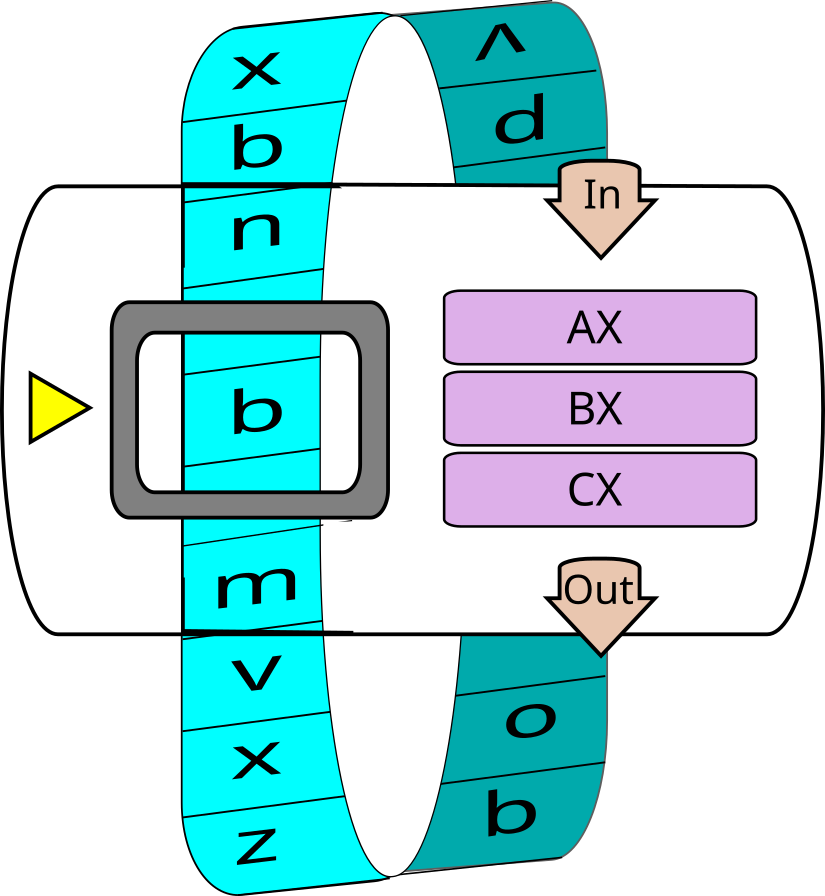
\includegraphics[width=0.5\columnwidth]{figures/methods/squishedCPU_extra.png}
\caption{{\bf An example virtual CPU from Avida}, with a circular genome (blue), three registers (purple), input and output handlers (tan), and an instruction pointer (yellow) indicating the next instruction to be executed.%
}\label{fig:cpu}
\end{figure}

%=description of Avida organism
An Avida organism is composed of a circular genome of assembly-like computer instructions that are executed in a virtual CPU (Fig~\ref{fig:cpu}). Populations of these organisms are placed in a toroidal world in individual cells where they are allowed to execute, reproduce, compete for space, mutate, and evolve.

% @CAO: I feel like a lot of this paragraph repeats information from the last section that was more generically about digital evolution.  We should probably tighten it up here.
%=Avida are self-replicating, but without perfect fidelity
Organisms in Avida are self-replicating, and experience mutation. The genome in the initial default organism contains all of the instructions necessary for reproduction. However, the instructions are not copied into an offspring with perfect fidelity. By default, the reproductive copy instruction is faulty, meaning that it will probabilistically introduce errors (mutations) into the offspring genomes. These offspring organisms execute their own genomes even when different from their parent, and in turn pass on their inherited mutations, along with new mutations, to their own offspring (i.e., variation in the systems is heritable).

%=Avida worlds are constrained and thus competition
Avida worlds can be space- or resource-constrained. Avida allows the experimenter to configure many aspects of the environment, thus subjecting the organisms to various kinds of selective pressures.  In many cases, these environments will include resources that can be metabolized by performing specific functions or activities, resulting in a boost to execution speed that gives the organisms a competitive advantage. However, even without explicit external pressures, organisms still experience an implicit pressure to execute more quickly and efficiently. The organisms that run fastest are typically able to also reproduce fastest, and thus out-compete their peers for space.

%=Avida and paper download information
%=[TODO - make the new git repos for the journal paper]
Avida is available for download without cost from \url{http://avida.devosoft.org/}, and specific versions along with data-files to reproduce the experiments described in this paper may be found at \url{https://github.com/voidptr/avida} and \url{https://github.com/voidptr/ce_evolvability}.

\subsection*{Experimental Design}
In order to examine the dynamics and mechanisms of evolving populations in changing environments, we performed a set of experiments divided into two stages. In the first stage, we subjected populations of evolving digital organisms to a set of benign and harsh cyclic changing environments. The cyclic environments were designed to simulate predictable cycles of change, such as day/night or seasonal cycles. These experiments allow organisms to adapt to a predictable set of environments, and explores short-term evolvability dynamics. See Table~\ref{ce-treatments-h}

The second stage takes these change-evolved populations and introduces them to a completely new environment. This set of experiments explores the relationship between evolvability traits acquired via selection for short-term adaptation to cyclical change, and examines how these traits perform in a long-term evolutionary context. See Table~\ref{cel-treatments-simple}.


% %from dis
% %In order to examine the dynamics and mechanisms of evolving populations in changing environments, we performed two sets of experiments. We subjected populations of evolving digital organisms to a set of cyclic changing environments, and a set stochastic changing environments. The cyclic environments were designed to simulate predictable cycles of change, such as day/night or seasonal cycles, whereas the stochastic environments represent less predictable oscillations in environmental states, such as random weather patterns, or climactic changes. These experiments allow organisms to adapt to a predictable set of environments, and explores short-term evolvability dynamics. See Table~\ref{ce-treatments-h}


% %=design for experimental environment (CCE vs SCE, and short vs long)
% In order to examine the dynamics and mechanisms of evolving populations in changing environments, we performed two sets of experiments.  

% In the first set, we compared cyclic changing environments vs stochastic changing environments. 
% %(cyclic vs stochastic changing environments), each divided into two phases (short-term evolvability vs. long-term evolvability). 
% The cyclic environments are designed to simulate predictable cycles of change, such as day/night or seasonal cycles, whereas the stochastic environments represents less predictable oscillations in environmental states, such as random weather patterns, or climactic changes. 

% In the second set of experiments, we allow organisms to adapt to a predictable set of cycling environments, and then introduce the change-evolved populations to a completely new environment. 

% Thus, the first set of experiments examines short-term evolutionary dynamics, and the second set explores the relationship between short-term adaptation to changing environments and long-term evolvability.

\subsubsection*{Short-Term Evolvability - Stage 1% - Cyclic Changing Environments
}

%=[TABLE - experimental treatments]
\begin{table}[]
\centering
\caption{\textbf{Experimental Treatments - Stage 1 - Cyclic Changing Environments}}
\label{ce-treatments-h}
\begin{tabular}{|c|c||c|c|}
\hline
\multirow{2}{*}{ \thead{Treatment} } & \multirow{2}{*}{ \thead{Changing \\ Environment} } & \multicolumn{2}{c|}{ \thead{Rewarded Tasks} } \\\cline{3-4}
& & \texttt{XOR} & \texttt{EQU} \\\hhline{|=|=|=|=|}
Control & \makecell{None \\ (static)} & \makecell{constant \\ $2^3$} & \makecell{constant \\ $2^5$} \\\hline
\makecell{Benign} & Cyclic & \makecell{constant \\ $2^3$} & \makecell{benign \\ fluctuating \\ 0 or $2^5$} \\\hline
\makecell{Harsh} & Cyclic & \makecell{constant \\ $2^3$} & \makecell{harsh \\ fluctuating \\ $-2^5$ or $2^5$} \\\hline
%\makecell{SCE \\ Benign} & Stochastic & \makecell{constant \\ $2^3$} & \makecell{benign \\ fluctuating \\ 0 or $2^5$} \\\hline
%\makecell{SCE \\ Harsh} & Stochastic & \makecell{constant \\ $2^3$} & \makecell{harsh \\ fluctuating \\ $-2^5$ or $2^5$} \\\hline
\end{tabular} 

\begin{flushleft} Two types of changing environment, plus a static control. In the first two treatments, the environment switches in a predictable cycle. The benign treatment enables and disables reward for the \texttt{EQU} task, while the harsh treatment rewards and then punishes this task.
\end{flushleft}
\label{ce-treatments}
\end{table}


%=explanation of the changing environment treatments - cyclic
We subjected a total of 150 replicate populations of digital organisms to two different treatments of two-phase cyclically changing environments, plus a static control. The environment cycles between equal-length periods of reward and punishment. Each cycle extends for 1000 updates, or roughly 30 generations. In the static control, there is no cycle. Rather, the rewards remain constant. This stage of the experiment extends for 200 cycles, or 200,000 updates, approximately 6,000 generations.

%=static env
In the static control, there is no cycle. Rather, the rewards remain constant. This stage of the experiment extends for 200 cycles, or 200,000 updates, approximately 6,000 generations.

% %=stochastic
% The stochastic changing environment experiment is similar to the cyclic environment, except that rather than the environment toggling every 500 updates, the environmental switch happens randomly, with a 0.002 probability of changing on every update. This averages, in the long term, to approximately one switch every 500 updates, but in the short term, the environmental switches are unpredictable.

%=tasks
We set up the system to detect organisms that performed \texttt{XOR} or \texttt{EQU}, two challenging bit-wise logical tasks. In the static control, \texttt{XOR} is rewarded with a CPU speed (and thus fitness) multiple of 8, while \texttt{EQU} is rewarded with a CPU speed multiple of 32. In the harsh treatment, as the cycle progresses, the \texttt{XOR} reward remains constant, while the \texttt{EQU} reward cycles between a 32-fold bonus and a correspondingly harsh 32-fold penalty (i.e., CPU speed is divided by 32 when \texttt{EQU} is performed in the off phase of the cycle). The benign treatment is nearly identical to the harsh treatment, except that the reward merely goes away in the off-cycle as opposed to incurring a severe penalty.

%=differences between tasks
In both environments, we identify \texttt{EQU} as the \textit{Fluctuating Task}. \texttt{XOR}, because it is rewarded continuously, is the \textit{Backbone Task}, and is used as a background for comparing the separation or intertwining of functional genetic components in the evolution of \texttt{EQU}. Further, the 4-fold difference in reward level between \texttt{XOR} and \texttt{EQU} encourages the evolution and maintenance of \texttt{EQU} when possible.

\subsubsection*{Long-Term Evolvability - Stage 2}
%=long term evolvability - new task
The second stage of the experiment continues the evolution of these populations, but introduces them to a completely new environment, with an expanded set of rewarded bitwise tasks to perform: Logic-77 (Table~\ref{cel-treatments-simple}). We refer to those tasks which were selected for in stage 1 as the \textbf{basic task set}. The Logic-77 task set is a super-set of the basic task set, and includes all bitwise tasks for which there are up to 3 inputs, including those that were initially rewarded in stage 1. We refer to the additional tasks from Logic-77 - those which are not part of the basic tasks set, and that we reward only in stage 2 - as the \textbf{expanded task set}. The total Logic-77 task set is a combination of both the basic and expanded task sets.  

	%=[TABLE - experimental treatments]
	\begin{table}[]
	\centering
	\caption{\textbf{Experimental Treatments - Stage 2 - Long Term Evolution}}
	\label{cel-treatments-simple-h}

	\begin{tabular}{|c|c||c|c||c|c|c|}
	%\begin{tabular}{ccccccc}
	\hline
	\multirow{3}{*}{ \thead{Treatment} } & \multirow{3}{*}{ \thead{Changing \\ Env. \\ Type} } & \multicolumn{5}{c|}{ \thead{Rewarded Tasks} } \\\cline{3-7}
	& & \multicolumn{2}{c||}{ \thead{Stage 1 \\ (0-200,000 Updates)} } & \multicolumn{3}{c|}{ \thead{Stage 2 \\ (200,000-400,000 Updates)} } \\\cline{3-7}
	& & \texttt{XOR} & \texttt{EQU} & \texttt{XOR} & \texttt{EQU} & \makecell{Expanded \\ Task-set \\ (Logic-77 \\ minus \\ \texttt{XOR} \& \texttt{EQU})} \\\hhline{|=|=|=|=|=|=|=|}
	Control & \makecell{None \\ (static)} & \makecell{constant \\ $2^3$} & \makecell{constant \\ $2^5$} & \makecell{constant \\ $2^3$} & \makecell{constant \\ $2^5$} & \makecell{constant \\ $2^{0.3}$} \\\hline
	Benign & Cyclic & \makecell{constant \\ $2^3$} & \makecell{benign \\ fluctuating \\ 0 or $2^5$} & \makecell{constant \\ $2^3$} & \makecell{benign \\ fluctuating \\ 0 or $2^5$} & \makecell{constant \\ $2^{0.3}$} \\\hline
	\makecell{Benign \\ Quiescent} & Cyclic & \makecell{constant \\ $2^3$} & \makecell{benign \\ fluctuating \\ 0 or $2^5$} & \makecell{constant \\ $2^3$} & \makecell{constant \\ $2^5$} & \makecell{constant \\ $2^{0.3}$} \\\hline
	Harsh & Cyclic & \makecell{constant \\ $2^3$} & \makecell{harsh \\ fluctuating \\ $-2^5$ or $2^5$} & \makecell{constant \\ $2^3$} & \makecell{harsh \\ fluctuating \\ $-2^5$ or $2^5$} & \makecell{constant \\ $2^{0.3}$} \\\hline
	\makecell{Harsh \\ Quiescent} & Cyclic & \makecell{constant \\ $2^3$} & \makecell{harsh \\ fluctuating \\ $-2^5$ or $2^5$} & \makecell{constant \\ $2^3$} & \makecell{constant \\ $2^5$} & \makecell{constant \\ $2^{0.3}$} \\\hline
	%\makecell{Harsh \\ to \\ Benign} & Cyclic & \makecell{constant \\ $2^3$} & \makecell{harsh \\ fluctuating \\ $-2^5$ or $2^5$} & \makecell{constant \\ $2^3$} & \makecell{benign \\ fluctuating \\ 0 or $2^5$} & \makecell{constant \\ $2^{0.3}$} \\\hline
	\end{tabular} 

	\begin{flushleft} Four types of cyclic changing environment, plus a static control. Each treatment is split into two stages. The first stage is a normal changing environment like those found in Table~\ref{ce-treatments-h}. The second stage introduces an additional set of tasks (the \textbf{expanded task set}) that are rewarded at a lower rate.
	\end{flushleft}
	\label{cel-treatments-simple}
	\end{table}

These new tasks use up to three bit-wise inputs rather than two, and are each rewarded with a constant 1.2-fold bonus to execution. This provides a mild selective pressure to evolve these tasks, but the benefits to performing them do not overwhelm the existing selective pressure to continue performing \texttt{XOR} or \texttt{EQU}.

In order to differentiate between the effects of architectural features and direct effects of alternating selection, we duplicated the populations in each the benign and harsh treatments at the end of stage 1 into two treatments each. Each treatment introduces the rewards of the \textbf{expanded task set}, but one treatment in each pair continues the changing environment of the first stage, while the other treatment stops the cycle, and instead rewards the \textbf{basic task set} at a constant rate.

\begin{itemize}
%@CAO: For each item in the list below it might be useful to start with a short sentence indicating WHY we did this treatment.
%@RCK: added
	\item \textbf{Static (Control)}: This treatment is a baseline for comparing adaptation to the \textbf{expanded task set}. For the first 200k updates (stage 1), we reward populations for performing  \texttt{XOR} and \texttt{EQU} (Table~\ref{cel-treatments-simple}). For the second 200k updates (stage 2), we add constant rewards for the \textbf{expanded task set}. Each new task is rewarded at a 1.2-fold bonus to task execution.

	\item \textbf{Benign Changing Environment}: This treatment shows the effects of a continuing benign changing environment on adaptation to the \textbf{expanded task set}. For the first 200k updates (stage 1), we alternate rewarding and not rewarding populations for performing the \texttt{EQU} task (Table~\ref{cel-treatments-simple}). For the second stage of the experiment, starting at 200k updates, we add constant rewards for each of the new tasks in the \textbf{expanded task set}, at a 1.2-fold bonus to task execution. The environmental fluctuation from the first stage continues through the end of the experiment.

	\item \textbf{Benign Quiescent Changing Environment}: In contrast to the benign changing environment treatment, this treatment tests the abilities of populations initially evolved in a benign changing environment to adapt to the \textbf{expanded task set}, but without active environmental fluctuation during the adaptation. For the first 200k updates (stage 1), we alternate rewarding and not rewarding populations, as in the Benign Changing Environment above. For the second stage of the experiment, starting at 200k updates, we add constant rewards for each of the new tasks in the \textbf{expanded task set}, at a 1.2-fold bonus to task execution. The environmental fluctuation from the first phase stops at 200k updates, and we instead reward the tasks of the first phase (the basic task-set) as we did in the static treatment (all constant reward).

	\item \textbf{Harsh Changing Environment}: This treatment shows the effects of a continuing harsh changing environment on adaptation to the \textbf{expanded task set}. For the first 200k updates (stage 1), we alternate rewarding and \textbf{punishing} populations for performing the \texttt{EQU} task (Table~\ref{cel-treatments-simple}). For the second stage of the experiment, starting at 200k updates, we add constant rewards for each of the new tasks of the \textbf{expanded task set}, at a 1.2-fold bonus to task execution. The environmental fluctuation from the first phase continues through the end of the experiment.

	\item \textbf{Harsh Quiescent Changing Environment}: In contrast to the harsh changing environment treatment, this treatment tests the abilities of populations initially evolved in a harsh changing environment to adapt to the \textbf{expanded task set}, but without active environmental fluctuation during the adaptation. For the first 200k updates (stage 1), we alternate rewarding and \textbf{punishing} populations, as in the Harsh Changing Environment above. For the second stage of the experiment, starting at 200k updates, we add constant rewards for each of the new tasks in the \textbf{expanded task set}, at a 1.2-fold bonus to task execution. The environmental fluctuation from the first stage stops at 200k updates, and we instead reward the basic tasks of the first phase as we did in the static treatment (all constant reward).
\end{itemize}




\subsection*{Measuring Task Discovery and Task Performance}
Task discovery and task performance are important measures not only of the adaptation of digital organisms to their local environment, but they also indicate the extent to which populations are more or less evolvable. Populations that are more evolvable should be able to acquire new tasks at a faster rate than less evolvable populations. If the evolvability of our populations is affected by evolution in a changing environment, then this effect should result in differential rates of task discovery and performance. Task discovery and performance together describe the exploration and exploitation of the environment by a population. 
% MJW: Added the "as detailed below" bit, because this is otherwise a bit abrupt. I mean, it still is, just less so.
%@RCK: reworded

\subsubsection*{Task Discovery}
Task discovery represents the level of exploration of the fitness landscape. We measured task discovery by counting the number of unique non-ephemeral tasks that have been discovered by a population. Each task may be performed only once per organism, yielding a maximum task count of 3600 at any given time. We define a non-ephemeral task as one that is performed by at least than 0.1\% of the population. 
%That is, at least 3.6 individuals (rounded up to 4) are performing the task at the time of sampling. 
Therefore, in order for a new task to be marked as discovered, it must be performed by at least 4 individuals at the time of sampling.

Once a task is discovered, it may not be un-discovered; task discovery counts will always increase monotonically. We measure \textbf{overall} task discovery by beginning to collect unique tasks starting at the beginning of the experiment. For the overall measurement, we count all possible tasks - the entire Logic-77 task set - even though not all tasks are rewarded in the first stage of the experiment. We also measure \textbf{post-reward} task discovery, where we begin counting new tasks from the beginning of the second stage of the experiment, once we have begun rewarding execution of the \textbf{expanded task set}. 
Task discovery can range anywhere from a minimum of zero tasks discovered, to a maximum of 77.
% MJW: I'd rephrase this to "rewards for the Logic-77 tasks". The way it is, it sounds like Logic-77 is not just an environment but also a specific reward scheme.
%@RCK: reworded to be clearer

\subsubsection*{Task Performance}
In addition to counting the number of unique task discovered, we also measure task performance. We measure task performance by counting the total number of unique, non-ephemeral tasks that a population is performing at each sampling point. This measure represents the level of exploitation of the fitness landscape. This measure can range from 0 to a maximum of 77 task being performed by the population. This value will always be either equal to, or smaller than the number of tasks discovered, since you can't perform a task you haven't discovered yet.   
% MJW: I think this is confusingly phrased. To the best of my understanding, you're saying that each task can only be performed once per organism. Therefore, for any given task, the maximum number of times it could be performed in a given update (which I'm guessing is your sampling?) is 3,600 (because I'm assuming that if a specific organism gives birth during the update and then somehow has enough cycles to perform that task again, it's still only counted as having happened once?). You therefore set a threshold at which tasks are only considered to be performed ephemerally, at 1 out of 100 organisms performing that task in the sampling. Anything performed more often than that is not ephemeral; you count the unique non-ephemeral tasks from the population as your measure of task performance. Introducing the term non-ephemeral several sentences before you define it is a bit confusing, and I'm still not entirely clear if you count whether organisms that are sampled *can* perform the task, or *do* perform the task at the point being sampled.
%RCK: No, it's the number of discovered tasks that the population has retained and is performing. Reworded for clarity.

%=the organisms
\subsubsection*{Experimental System}
%\todo[inline]{fix the title to be about the details of the system}
For all of the experiments described in this paper, we held the individual genomes at a fixed length of 121\footnote{As part of our initial controls, we hand-wrote an organism with separated sections that performed \texttt{XOR} and \texttt{EQU}. This hand-written organism had 121 instructions and as such we used this genome length as a constraint for the evolved organisms as well.} instructions, but tested the new genomes for mutations after each successful replication event at a substitution probability of 0.00075 per site. 

We configured the Avida world to have local interactions on a toroidal grid that is 60-by-60 cells (3600 cells in total), and we seeded the initial populations with an ancestor that was previously evolved to perform \texttt{XOR} and \texttt{EQU} under a static reward. The genetic architecture for performing \texttt{XOR} and \texttt{EQU} is tightly intertwined in this ancestral organism, as it was evolved with no selective pressure for modularity.

\subsection*{Statistical Methods}
Most of the statistical techniques used in this paper are non-parametric, and focused on differentiating between sample distributions. In general, we applied Wilcoxon Rank-Sum tests~\cite{wilcoxon_individual_1945} to distinguish between pairs of distributions, as well as Kruskal-Wallis~\cite{kruskal_use_1952} for identifying whether we could reject the null hypothesis of sameness between several different distributions. We assume all distributions are independent, and that compared distributions have similar shapes. In all situations where there were multiple comparisons of a given distributions, we applied Bonferonni corrections~\cite{rice_analyzing_1989} before assessing statistical significance. 

In certain cases, we report mean and median values of distributions. In these cases, we also report the standard deviation or 95\% confidence intervals.

In specific cases, we also apply Spearman's rank-order correlation coefficient $\rho$ (or $r_{s}$)~\cite{spearman_proof_1904} to measure correlations between data sets. In all cases, data points are matched from within a replicate.

\section*{Results and Discussion}
%\todo[inline]{note about long-term evo stuff}
%=summary - we found that CE evolved populations are genetically distinct. Stochastic pretty similar to CCE
Our experiments (detailed below) demonstrate that digital organisms that were evolved in changing environments differ substantially from those that evolved in static environments in a number of ways. These differences include the number of mutations that fix in the lineage from the ancestor (the ``phylogenetic depth"), key metrics of their genetic architecture, and the presence of reservoirs of pseudogenes that change the nearby mutational landscape. These features represent adaptation to the larger regime of repeated environmental switching. 
%We also show that while populations evolved in cyclic environments are slightly better adapted to change than those that evolved in stochastic environments, in most measures of adaptation and short-term evolvability, these differences are generally not significant. This result indicates that while regular periodicity may offer a slight advantage for adaptation, stochastic environments perform similarly in most respects. 
%\todo[inline]{look for un-anchored "this"s}

We also show that while harsh changing environments are better at promoting short-term adaptation to changing environments, benign environments produce populations that adapt more rapidly to entirely new sets of tasks. This suggests that the selective pressures that promote short-term adaptation are not necessarily the same as those that promote long-term evolvability.

\subsection*{Stage 1 - Cyclic Changing Environments}
We will begin by examining the characteristics of populations evolved in cyclic changing environments.

\subsubsection*{Performance of \texttt{EQU}}
Each population was seeded with organisms that performed both the \texttt{EQU} fluctuating task, and the \texttt{XOR} backbone task. We measured the execution of the \texttt{EQU} task, and observed that in the static control treatment, \texttt{EQU} is fixed in the population and remains so throughout the run. In contrast, we observed a periodic dip in the execution of \texttt{EQU} in the benign changing environment during the non-rewarded phase of the cycle, followed by a rapid recovery when rewards are reinstated. Finally, in the harsh treatment, we observed abrupt disappearance of \texttt{EQU} performance, followed by rapid recoveries, coinciding with phases of reward and punishment. As expected, these results suggest that the populations are responding to the selective pressures to perform \texttt{EQU} when it is rewarded, and to lose functionality when it is not rewarded or when it is punished.

%\todo[inline]{Show figure of early vs late adaptation}
%=[FIGURE - functional vs vestigial sites]
	\begin{figure}[!h]
	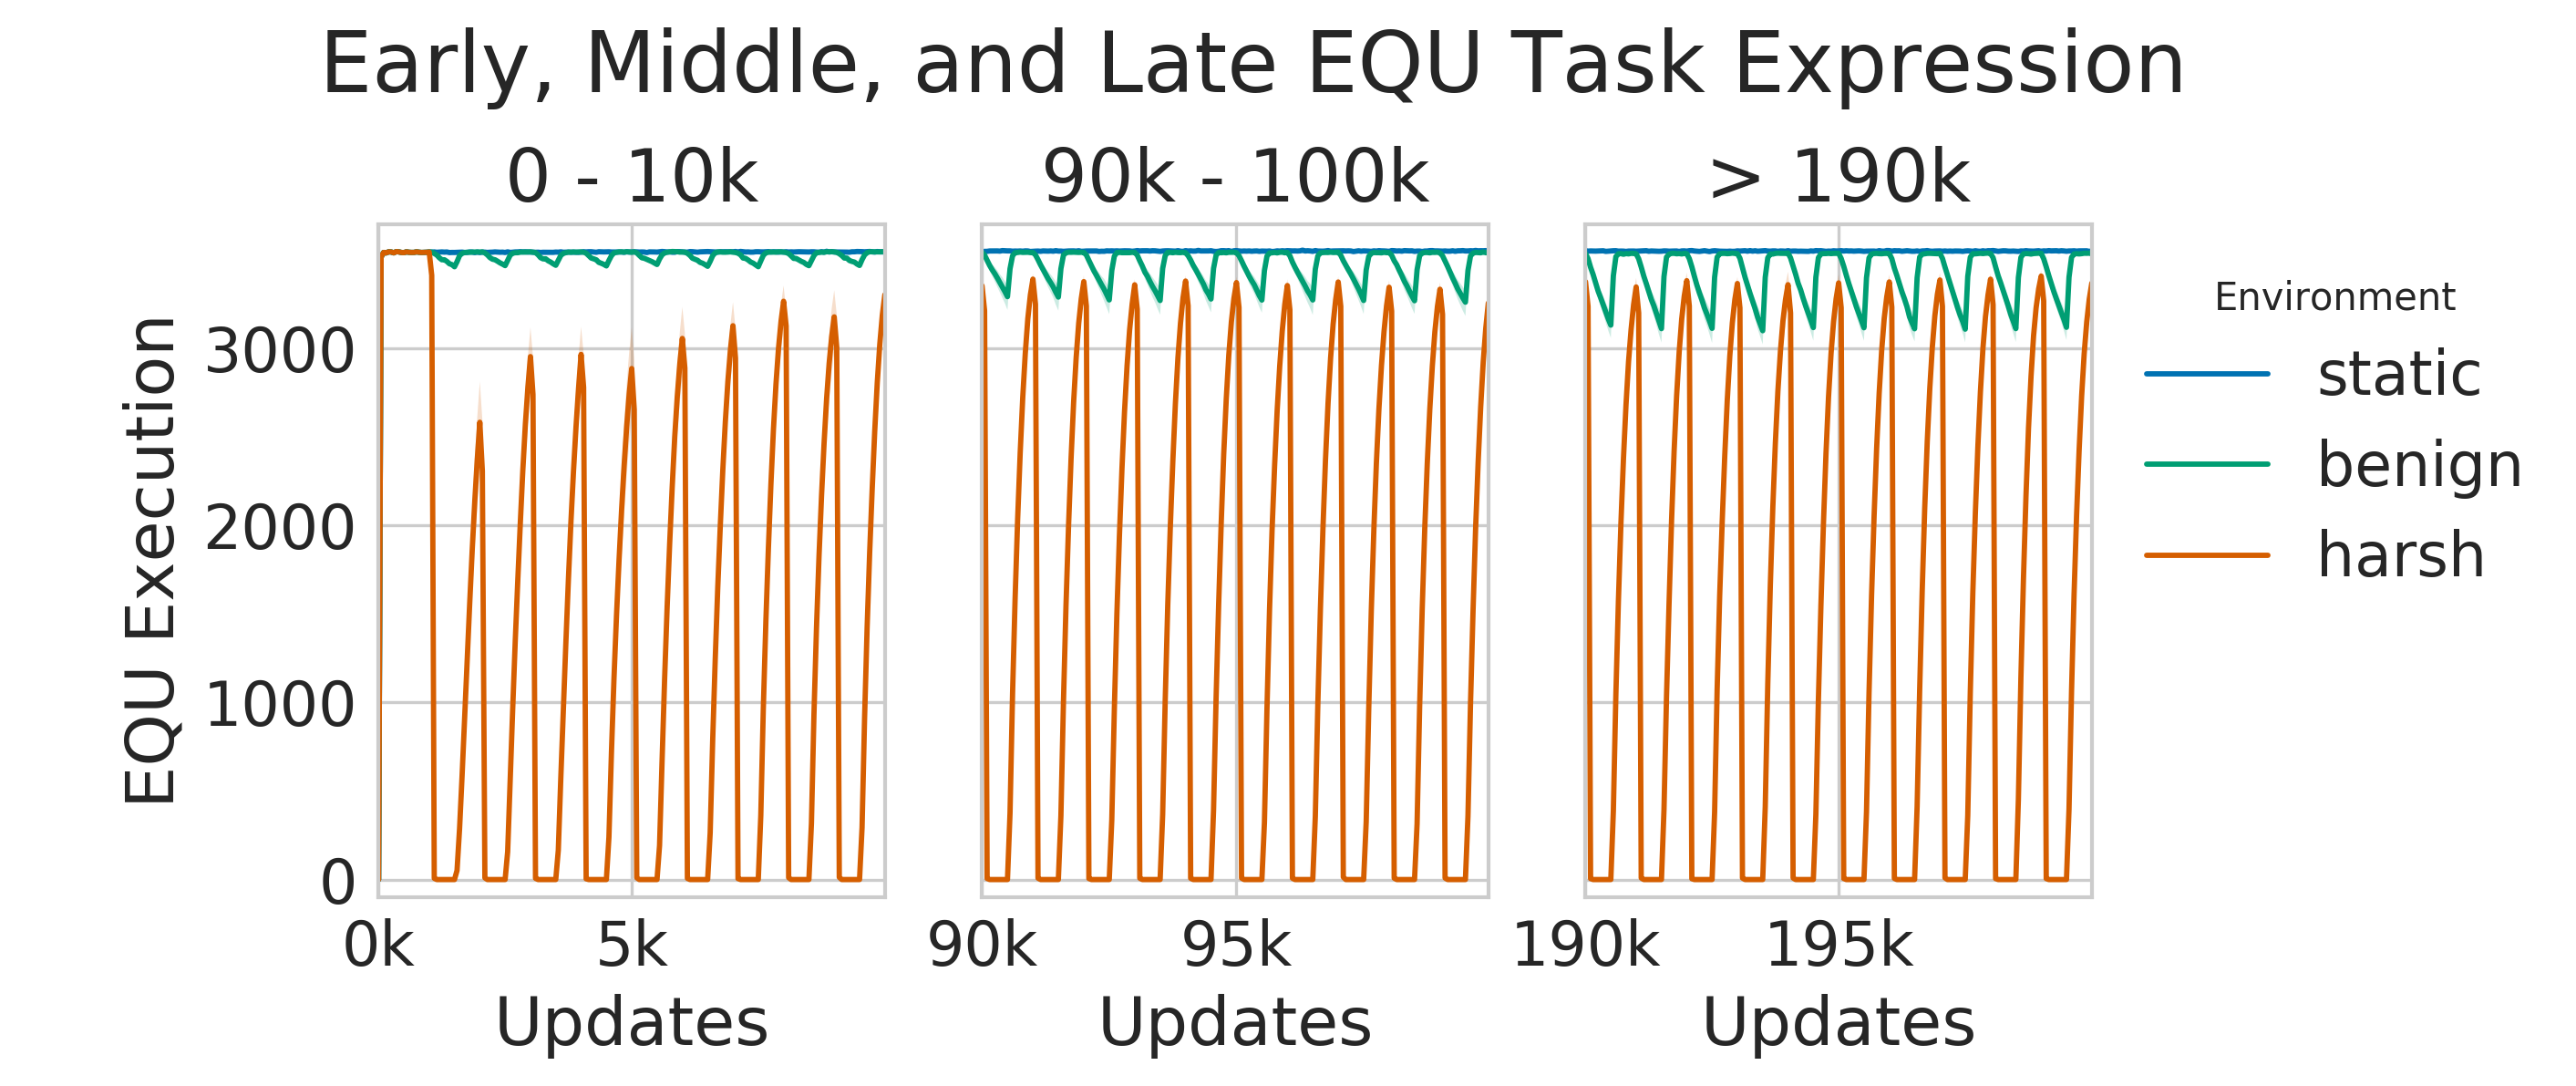
\includegraphics[width=0.95\columnwidth]{figures/CE/CCE_equ_execution.png}
	\caption{\textbf{Number of organisms performing \texttt{EQU} task}. We measured the execution of the \texttt{EQU} task in all treatments. In the benign treatment, we observed increasing periodic dips in execution that coincide with phases of non-reward as the experiments progressed. In the harsh treatment, we observed adaptation, resulting in abrupt disappearance of \texttt{EQU} in the punishment phase, followed by rapid recovery of \texttt{EQU} performance during the reward phase.
	}
	\label{fig:CCE_equ_execution} %% FIGURE 5
	\end{figure}

\subsubsection*{Evolutionary History and Population Structure}
%=more phylogenetic depth
We then surveyed the evolutionary history and population structure of the evolving populations. Evolution in the harsh cyclic changing environment resulted in many more mutations fixing, and thus populations with substantially higher phylogenetic depth as compared to those evolved in static or benign environments. At each environmental shift, adaptive mutations rapidly swept and fixed in the populations. (Fig~\ref{fig:flamegraph})

	%=[FIGURE - flamegraph]
	\begin{figure}[!h]
	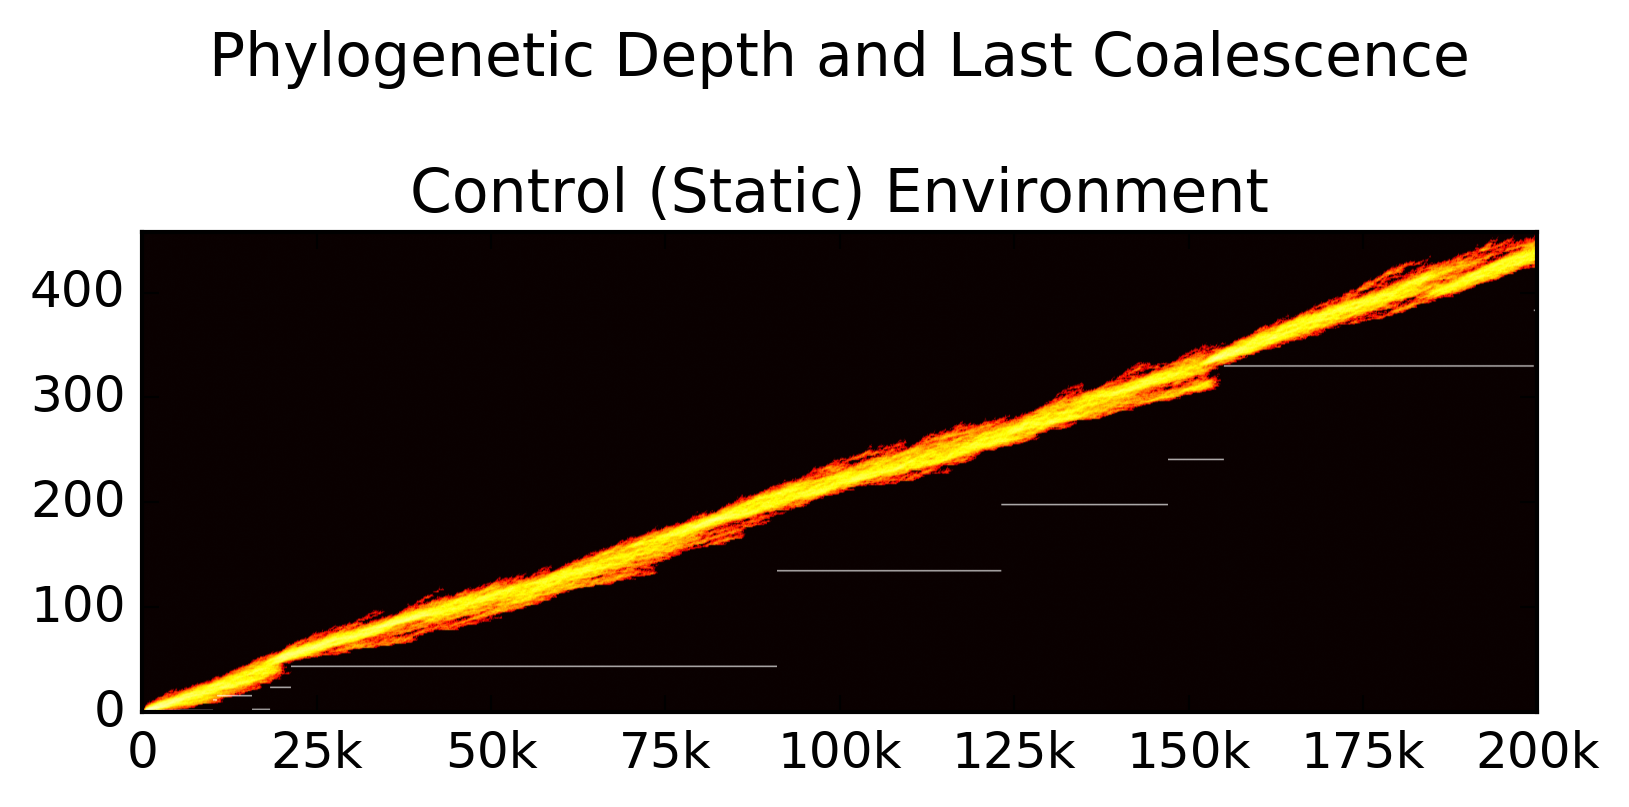
\includegraphics[trim={-0.88cm 0 0.25cm 0},clip,width=0.65\columnwidth]{figures/CE/control__phylodepth_with_coalescense.png}

	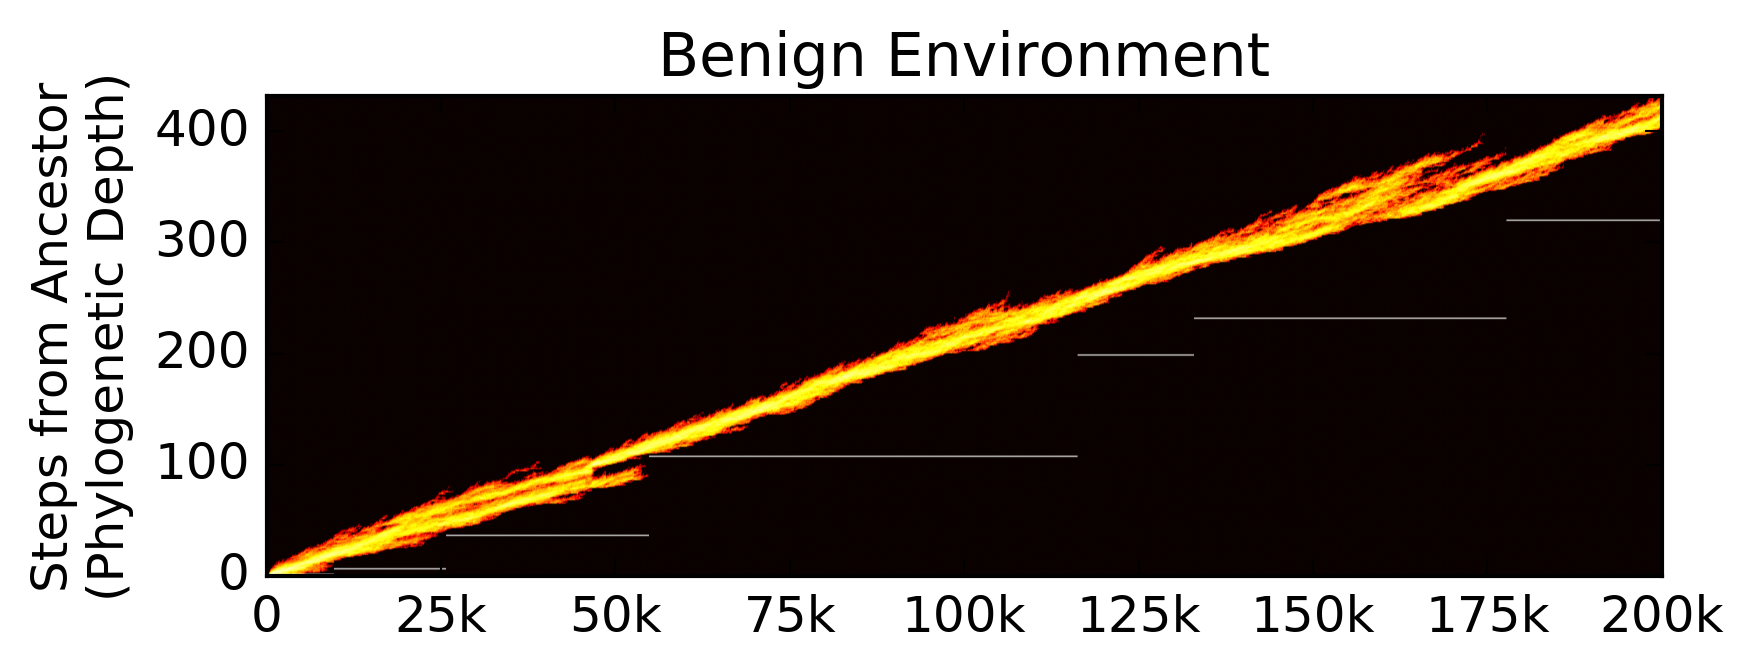
\includegraphics[trim={0.2cm 0 0.25cm 0},clip,width=0.65\columnwidth]{figures/CE/benign__phylodepth_with_coalescense.png}
	
	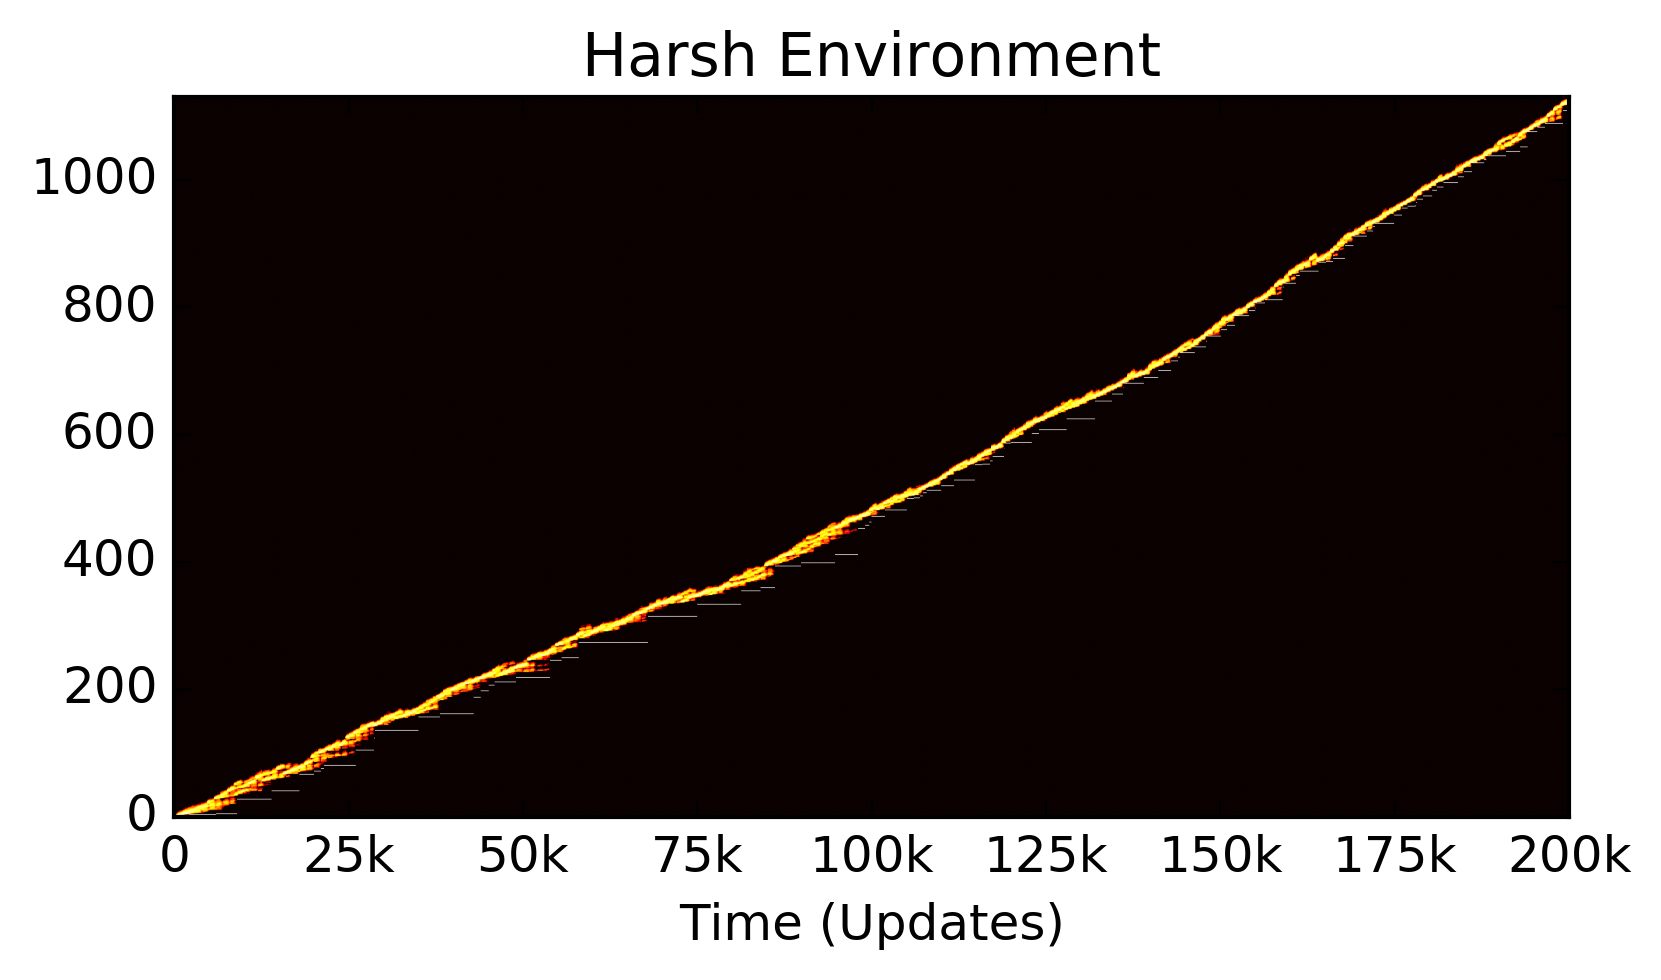
\includegraphics[trim={-0.63cm 0 0.25cm 0},clip,width=0.65\columnwidth]{figures/CE/harsh__phylodepth_with_coalescense.png}
	\caption{\textbf{Phylogenetic depth over time} of a sample population evolved in each of the three treatments of the cyclic changing environments. White horizontal lines mark the depth of the most recent common ancestor, and discontinuities in this line indicate that the most recent common ancestor has changed, and thus that a sweep occurred, or that a competing clade went extinct. The control treatments had a mean of 18 sweeps (STD=9.05), the benign treatments had a mean of 21 (STD=19.05), and the harsh treatments had a mean of 88 sweeps (STD=23.37). Note the difference in scales between y-axes: the control-evolved population has a maximum depth of 400 mutational steps from ancestor, while the harsh-evolved has upward of 1100. %
	}\label{fig:flamegraph}
	\end{figure}

%=more genetic diversity
The populations that evolved in the control and benign environments displayed more genetic diversity as compared to those evolved in the harsh cyclic environment, which underwent a bottleneck at each cycle shift (see Fig~\ref{fig:population-entropy}). Because a selective sweep reduces current diversity within a population, the smaller number of sweeps
% @CAO it looks like it wasn't just a smaller number of sweeps, but that the sweeps took MUCH longer to occur, to the point where it's hard to even dub them sweeps at all... more fixation events?  Mike should weigh in here too.
in the benign and control treatments led populations in them to have higher standing diversity for most of their evolutionary history than those populations from the harsh changing environment. Despite this higher standing diversity in the benign and control treatments, regions of low diversity are still evident in the genomes of these populations, implying purifying selection on the traits encoded at these sites (see Fig~\ref{fig:by-site-entropy}).
% * <mjwiser@gmail.com> 2017-01-30T19:39:00.542Z:
%
% I feel like this figure would be easier to talk about if you split it into three panels, and mention that each panel has both an upper and a lower part. It would also probably be easier to read if the axes on the left were on the top panel, rather than the middle one; since you have two graphs in each panel, it doesn't make sense to just have a single axis label off to the side. However, you probably *can* have only a single x axis label, since the axes are the same for all the panels, and for both graphs within a panel.
%
% ^.

	\begin{figure}[!h]
	%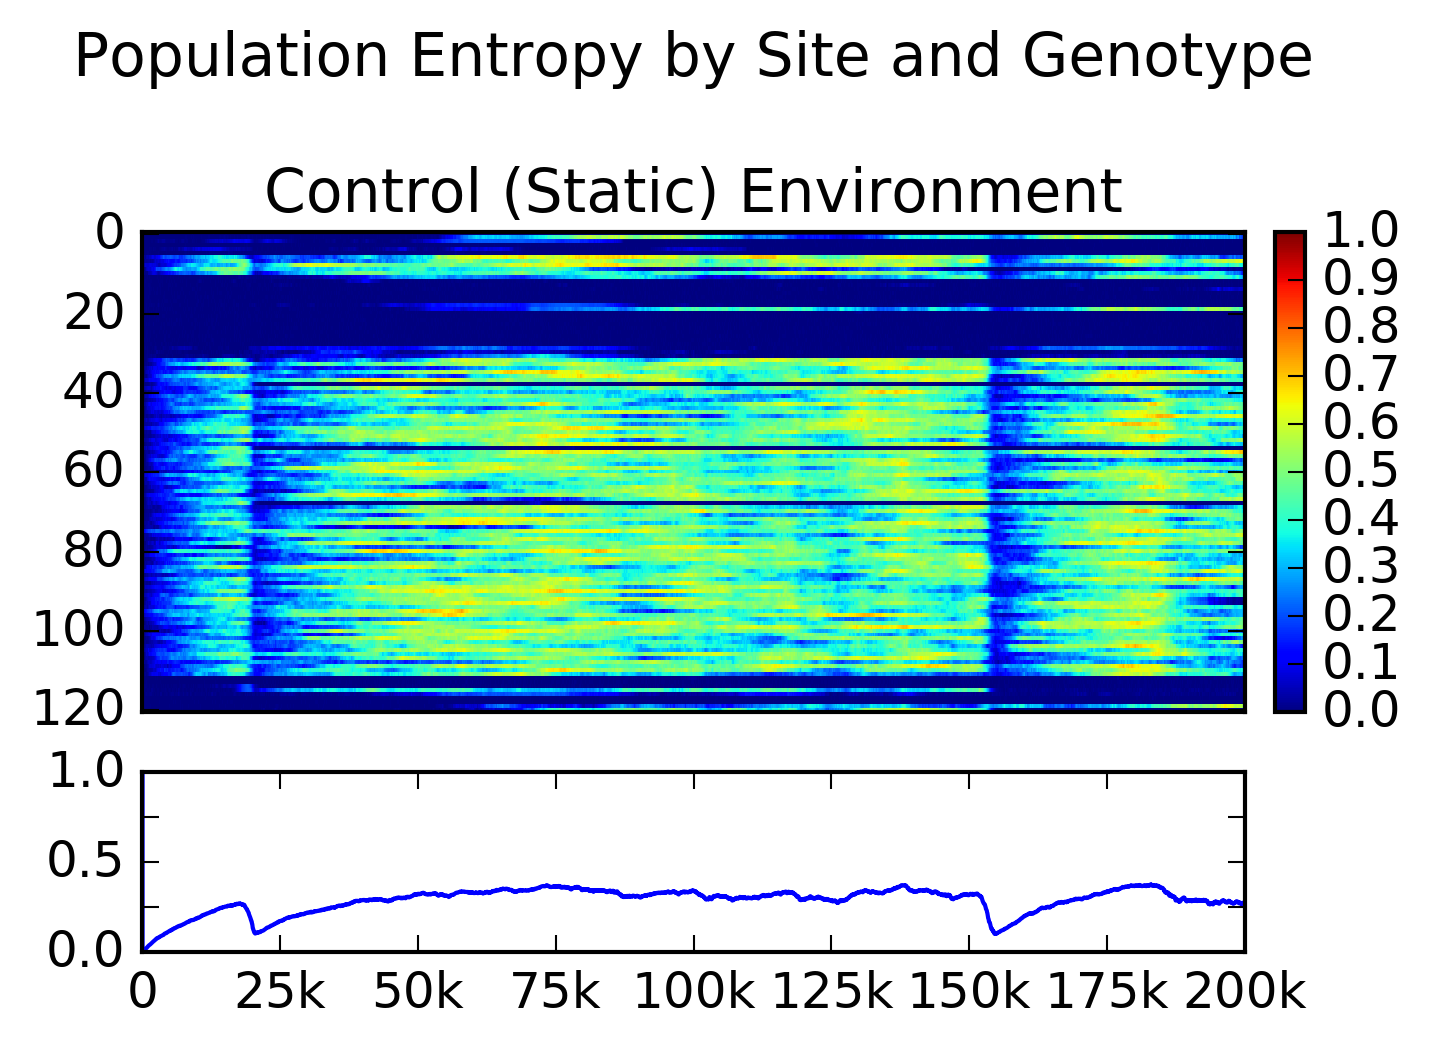
\includegraphics{figures/CE/control__entropy}
	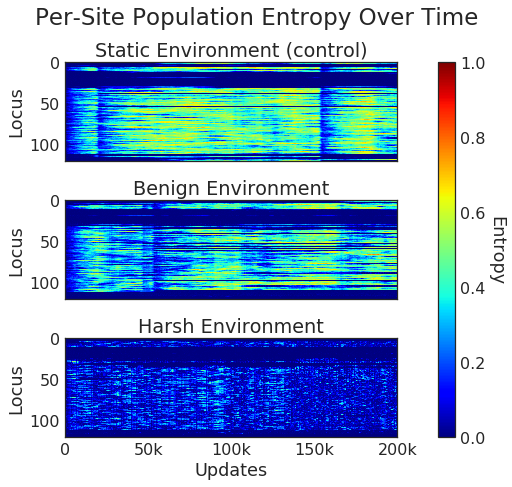
\includegraphics[width=0.75\columnwidth]{figures/CE/by_site_entropy}
	\caption{\textbf{Per-site entropy over time} of a representative sample population. Each vertical slice represents the per-site entropy of the population at each update by genetic locus. Hotter colors (red/orange/yellow) indicate greater diversity at this locus, while cooler colors (blues) indicate the a locus is more consistent across the population.   %@CAO: I'm agreeing with Mike that we might want to make this two graphs. I added a bit in the description about the cooler colors just to lead the reader by the hand as much as possible.
	}\label{fig:by-site-entropy}
	\end{figure}

	\begin{figure}[!h]
	%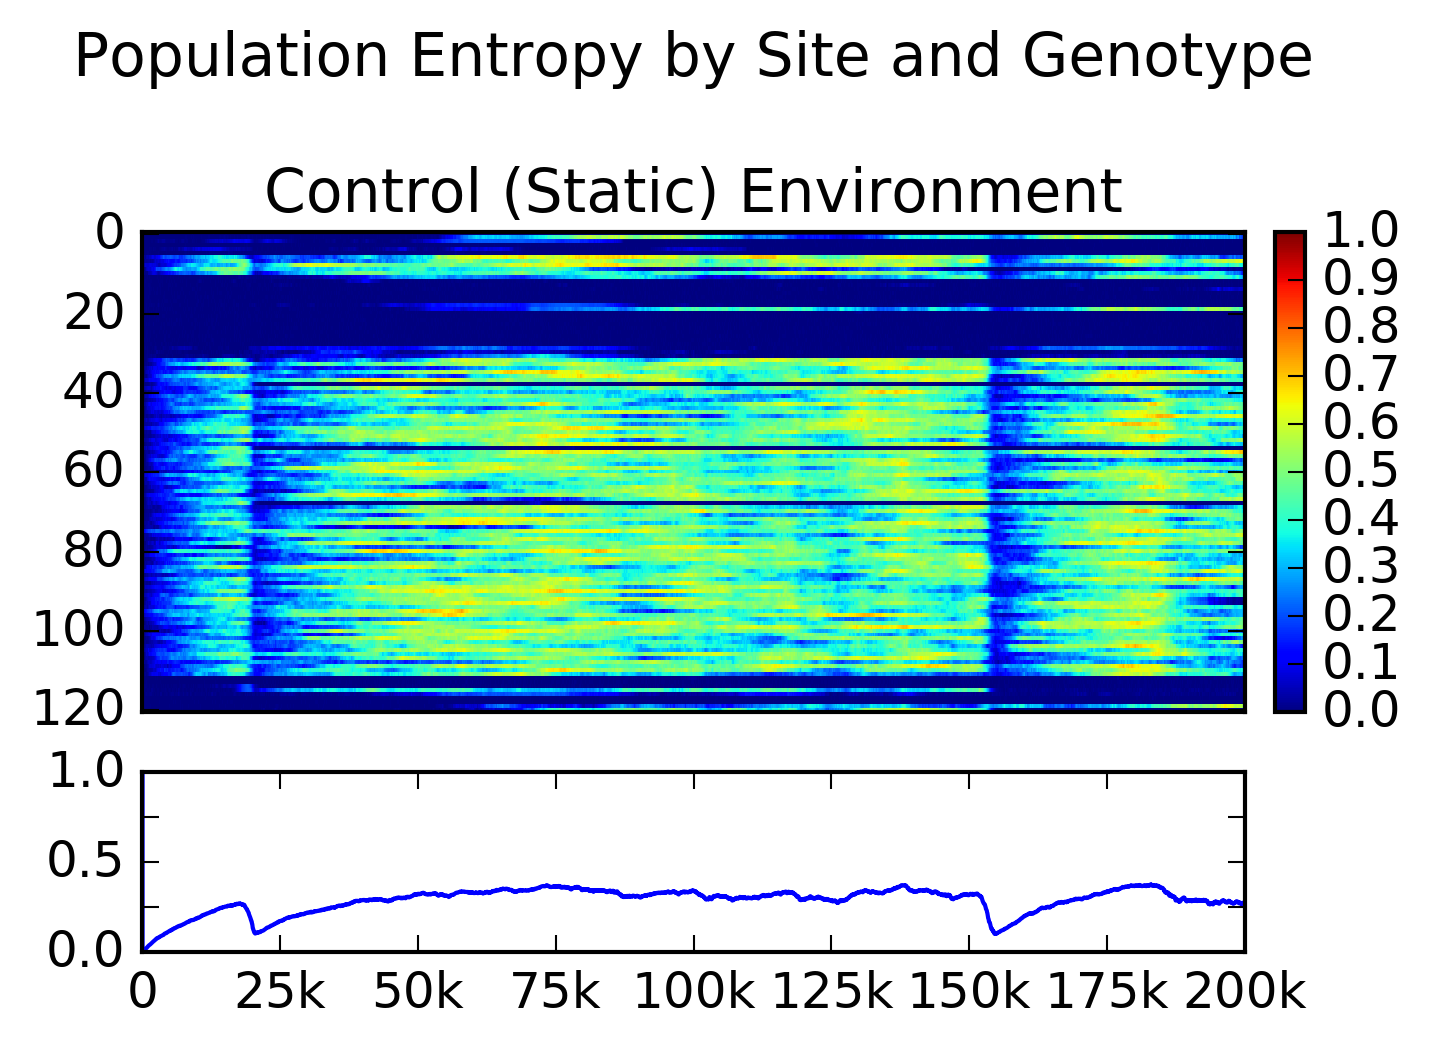
\includegraphics{figures/CE/control__entropy}
	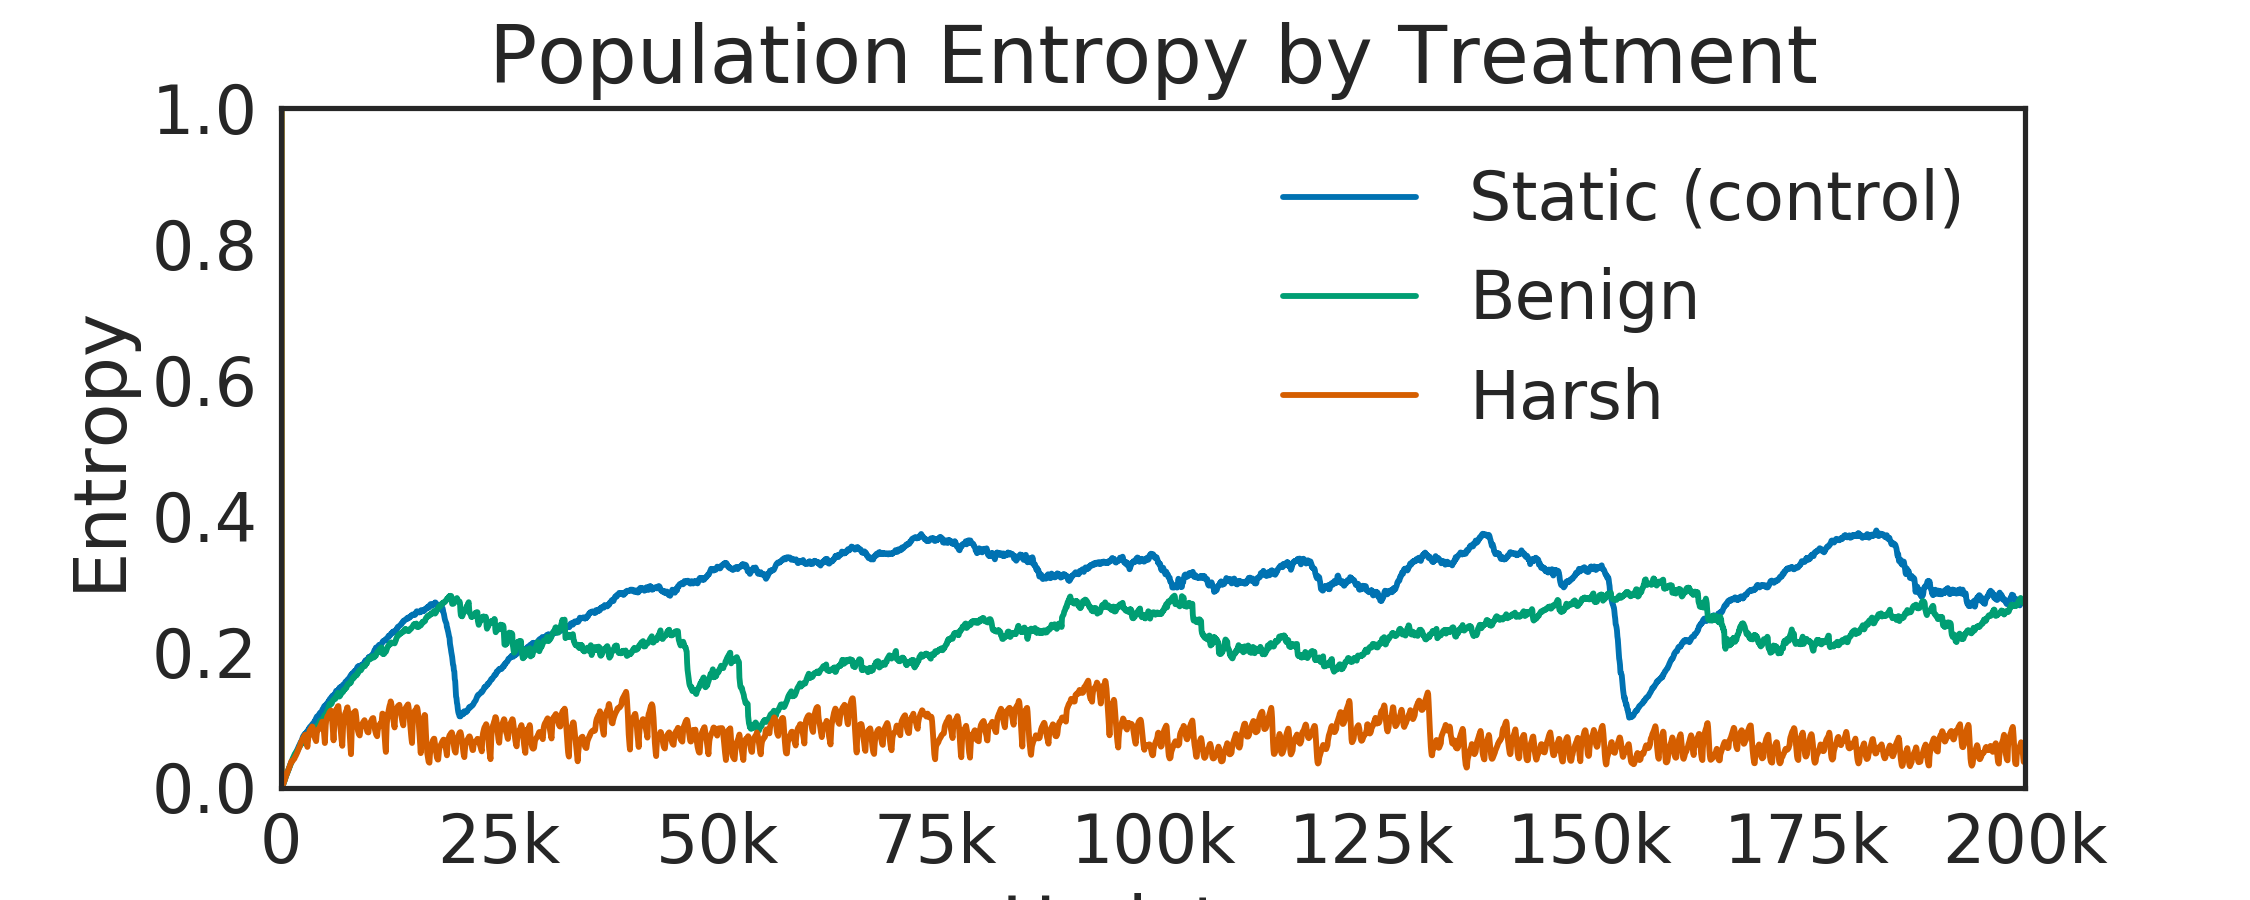
\includegraphics[width=0.75\columnwidth]{figures/CE/population_entropy}
	\caption{\textbf{Population entropy over time} of the representative sample population in Figure~\ref{fig:by-site-entropy}. Mean population entropy indicates the relative diversity of the population at any given time, while the per-site entropy (see Fig~\ref{fig:by-site-entropy}) shows where in the genomes the population diversity is located.   %@CAO: I'm agreeing with Mike that we might want to make this two graphs. I added a bit in the description about the cooler colors just to lead the reader by the hand as much as possible.
	}\label{fig:population-entropy}
	\end{figure}

% \todo[inline]{fix figure below so that it's two separate figures. Separate the mean entropy to its own figure.}
% 	\begin{figure}[!h]
% 	%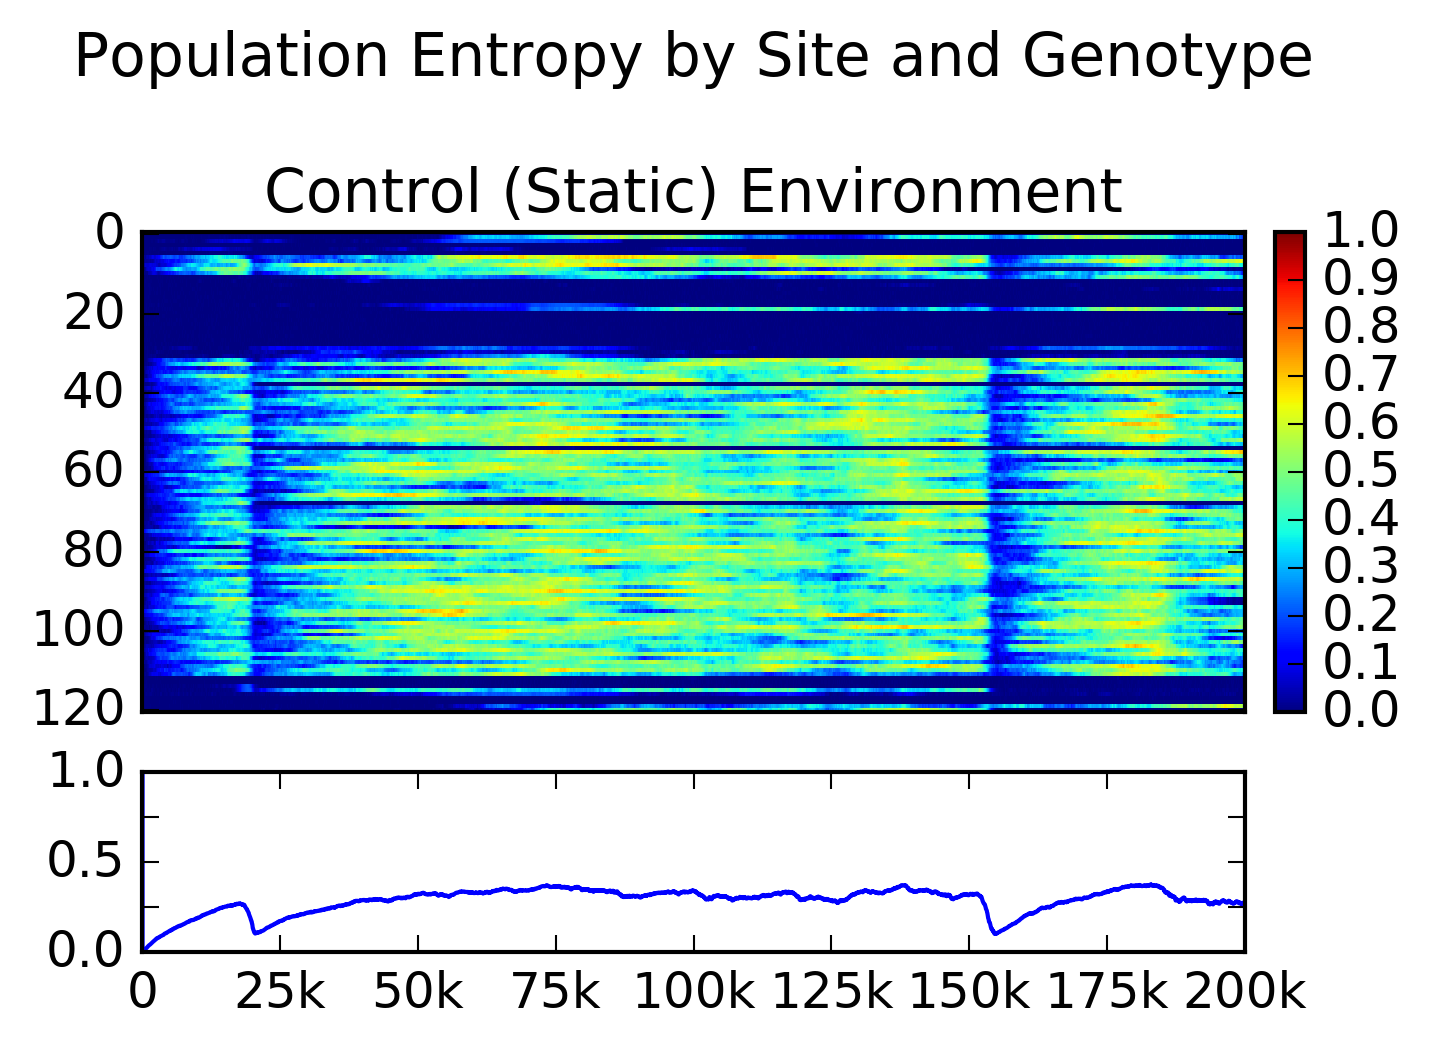
\includegraphics{figures/CE/control__entropy}
% 	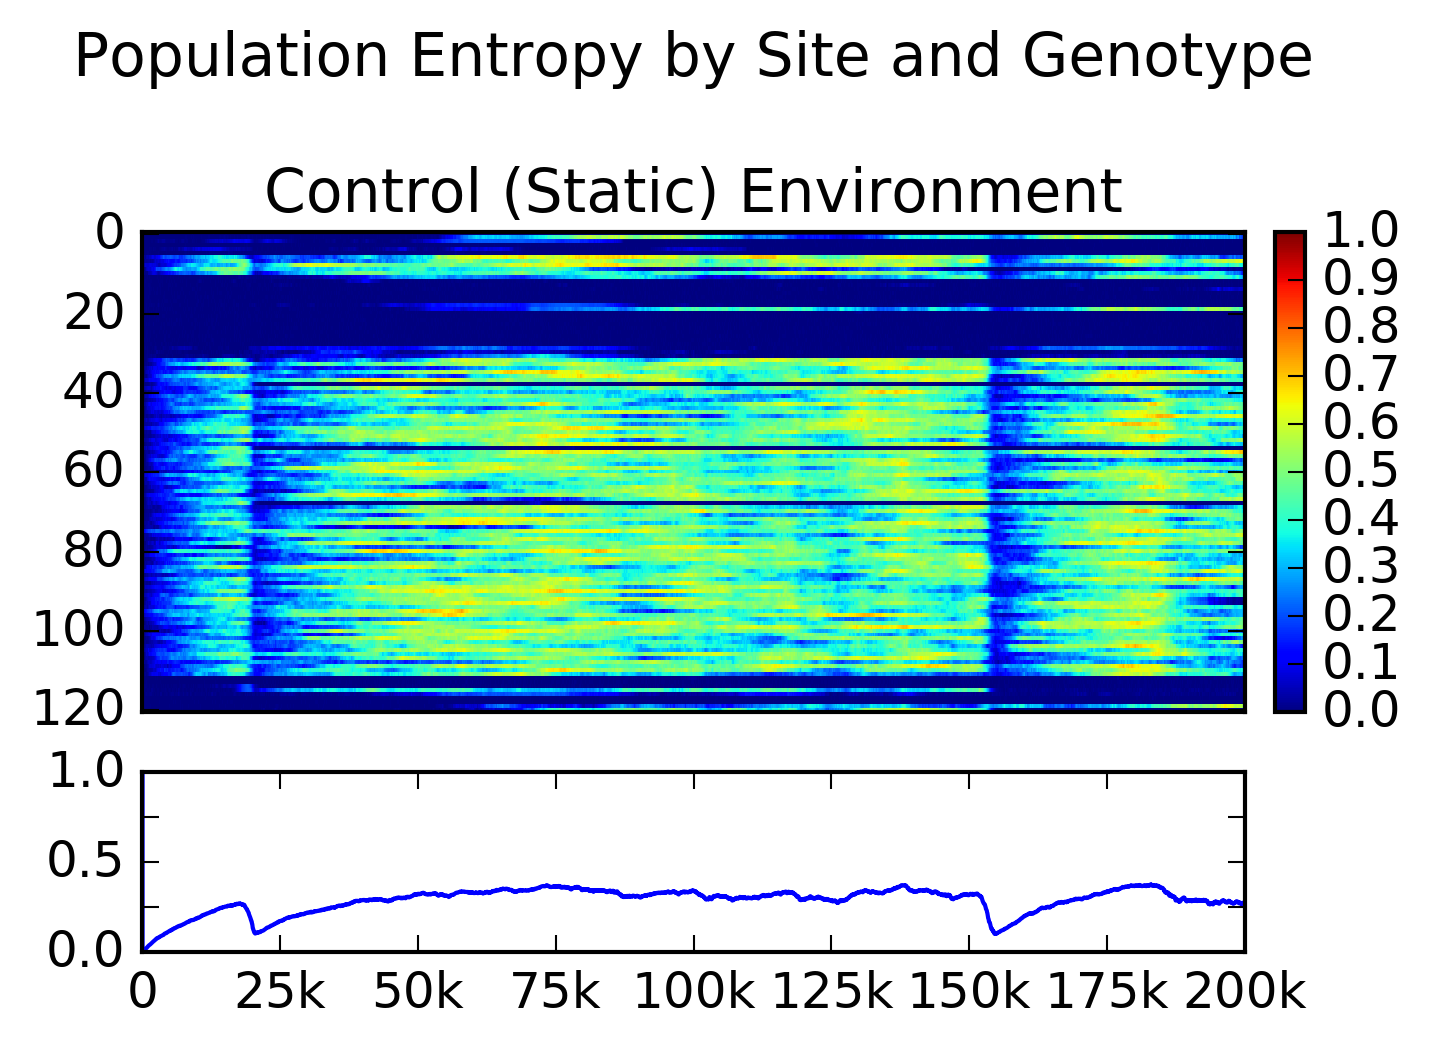
\includegraphics[trim={-0.85cm 0 0.1cm 0.2cm},clip,width=0.5\columnwidth]{figures/CE/control__entropy}
% 	%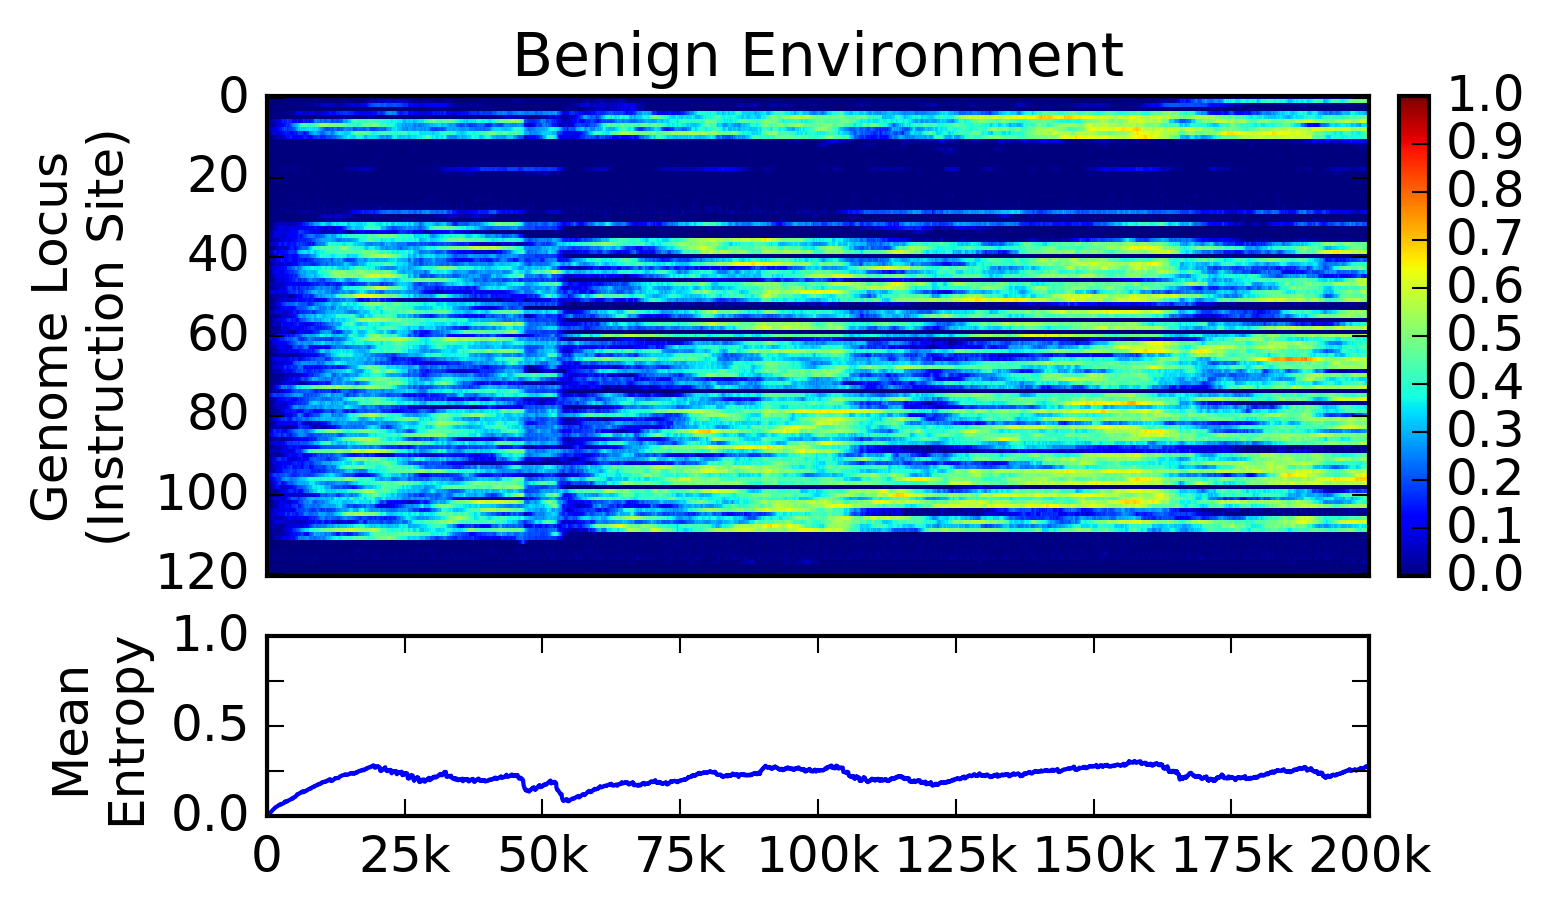
\includegraphics{figures/CE/benign__entropy}
% 	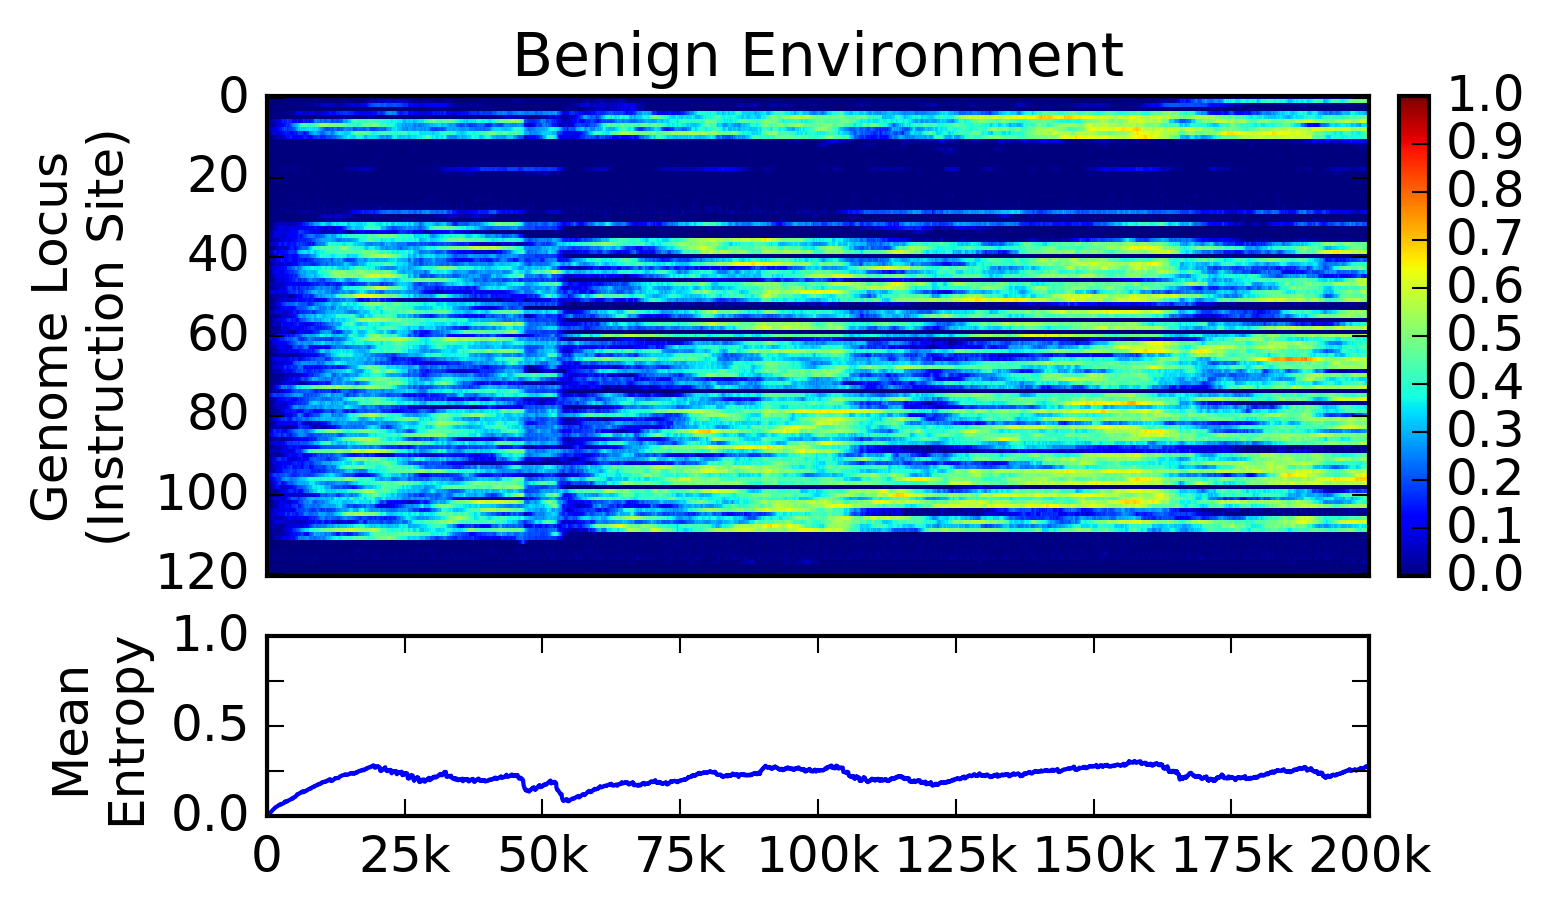
\includegraphics[trim={0.25cm 0 0.1cm 0},clip,width=0.5\columnwidth]{figures/CE/benign__entropy}
% 	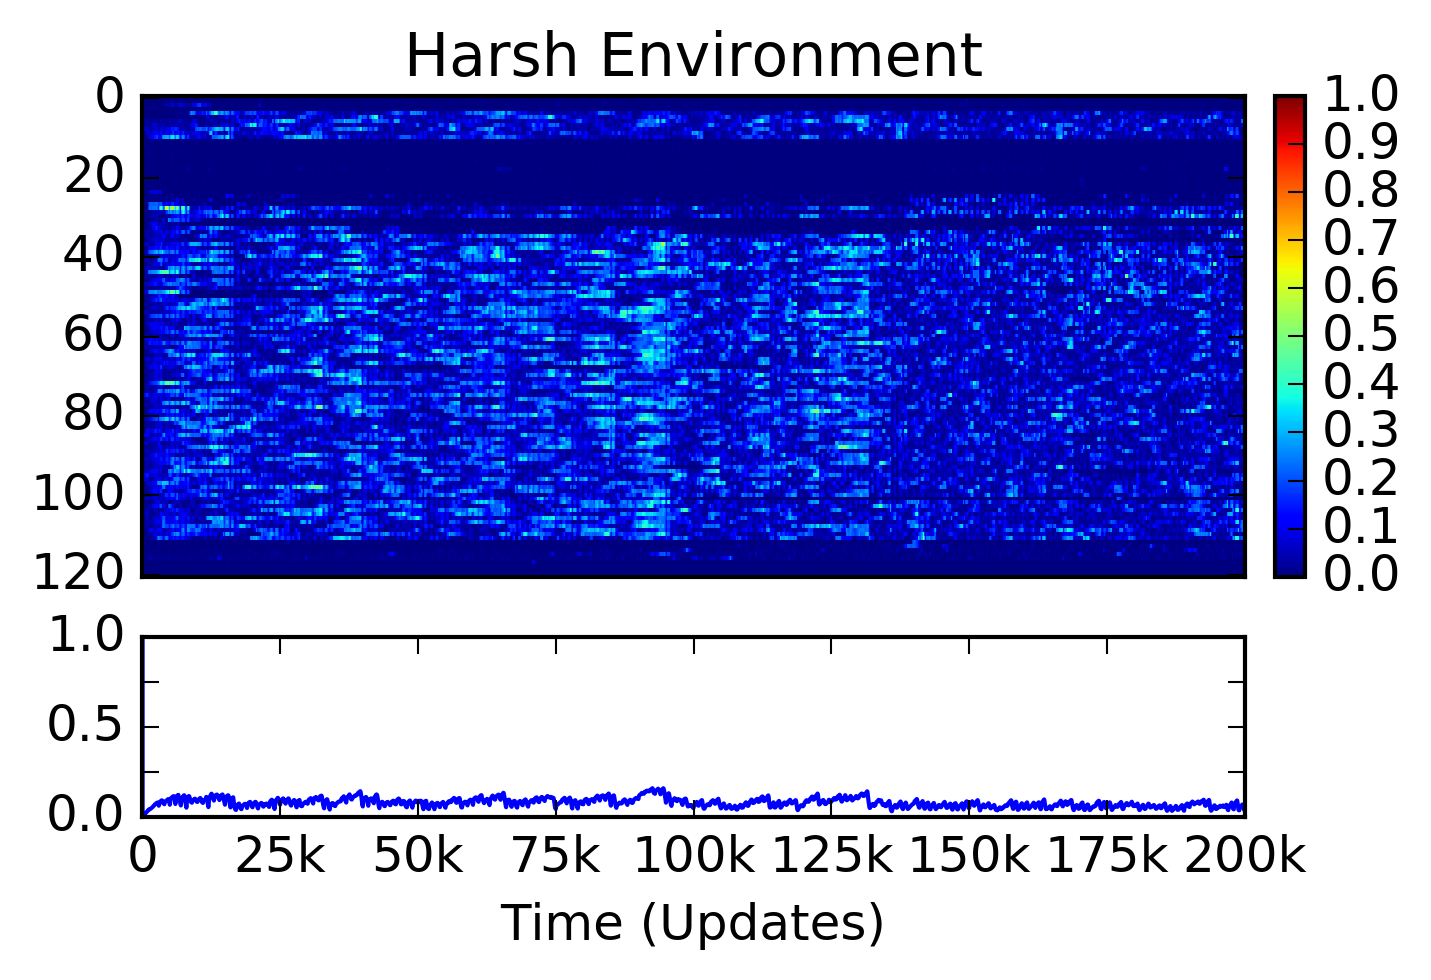
\includegraphics[trim={-0.85cm 0 0.1cm 0},clip,width=0.5\columnwidth]{figures/CE/harsh__entropy}
% 	\caption{\textbf{Population Per-site Entropy over time} of a representative sample population. Each vertical slice represents the per-site entropy of the population at each update, both by genetic locus (upper), and overall population mean (lower). Hotter colors (red/orange/yellow) indicate greater diversity at this locus, while cooler colors (blues) indicate the a locus is more consistent across the population. Mean population entropy indicates the relative diversity of the population at any given time, while the per-site entropy shows where in the genomes the population diversity is located.   %@CAO: I'm agreeing with Mike that we might want to make this two graphs. I added a bit in the description about the cooler colors just to lead the reader by the hand as much as possible.
% 	}\label{fig:entropy}
% 	\end{figure}


\subsubsection*{Genetic Architecture}
%=genetic architecture is different in benign and harsh vs control
The alternating selection in both benign and harsh changing environments results in qualitatively different architectural styles as compared with those genomes evolved in the static environment. The task arrangements evolved under both experimental treatments are much more scattered throughout the genome than in the control, which is tightly compacted. Specifically, the bulk of the sites responsible for performing the fluctuating task (\texttt{EQU}) did not overlap with the backbone task (\texttt{XOR}), except for a small core region, which represents portions of the tasks that are shared between \texttt{XOR} and \texttt{EQU}. That is, in the changing environment treatments, we see many more sites that only code for a single task, whereas in the static treatment, the majority of functional tasks sites code for both \texttt{XOR} and \texttt{EQU}. (See Figs~\ref{fig:lineage-control}, \ref{fig:lineage-benign}, and \ref{fig:lineage-harsh})
% @CAO: I'm not positive I understand this description for how things are laid out. It might be worth putting a bit more detail here, and highlighting also that there is a lot more separation in the harsh environment (or so it seems). Should we talk more here about why all of this is the case (highlighting that we are speculating) or will that come later?
%@RCK: Reframed to clarify.

% \todo[inline]{polish this figure, task layout, make three separate figures}
% 	\begin{figure}[!h]
% 	\setlength{\fboxsep}{0pt}%
% 	\setlength{\fboxrule}{0pt}%
% 	\fbox{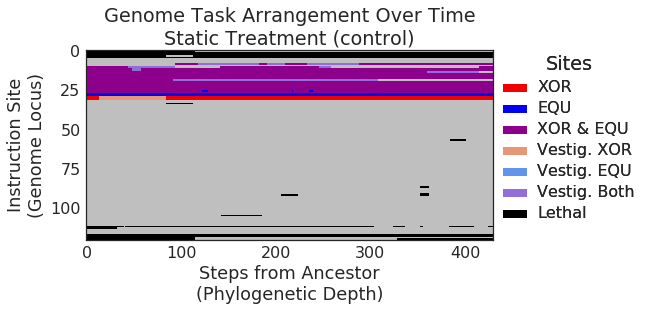
\includegraphics[width=0.5625\columnwidth,trim={-0.82cm 0 5.5cm 0.25cm},clip]{figures/CE/control__whole_taskmap.png}}\fbox{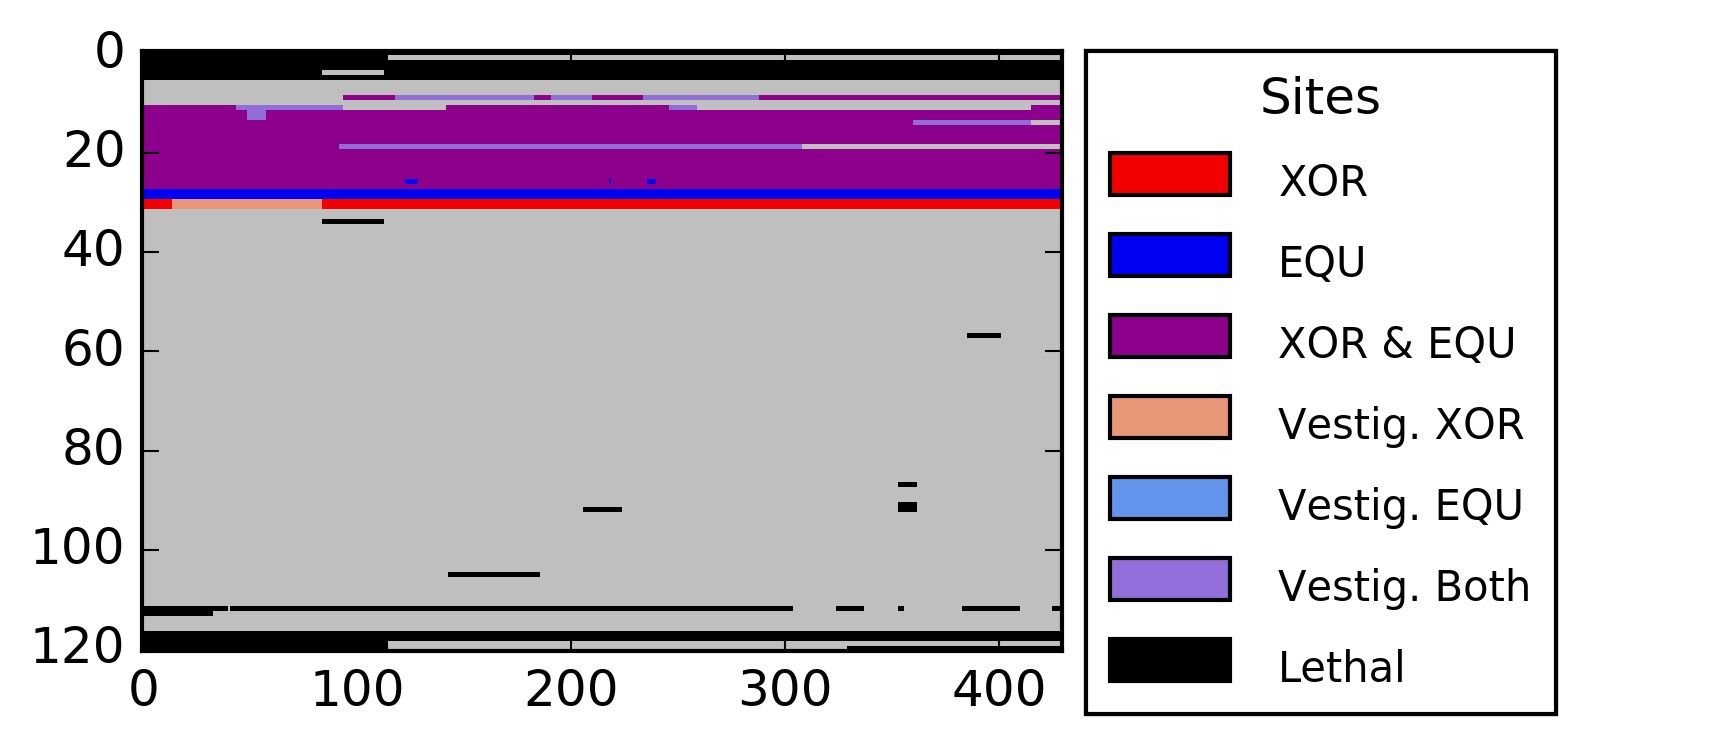
\includegraphics[width=0.1875\columnwidth,trim={9.1cm 0.15cm 1.3cm 0},clip]{figures/CE/legend__whole_taskmap.png}}
% 	\fbox{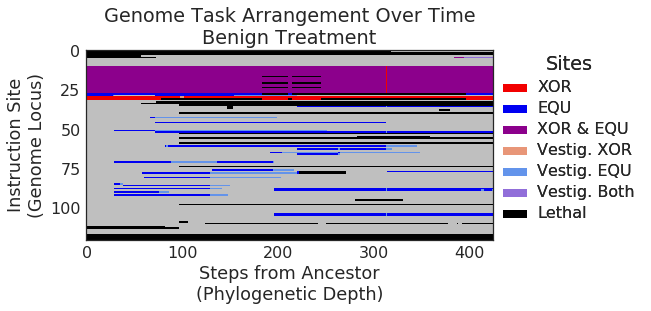
\includegraphics[width=0.75\columnwidth,trim={0.2cm 0 2.3cm 0},clip]{figures/CE/benign__whole_taskmap.png}}
% 	\fbox{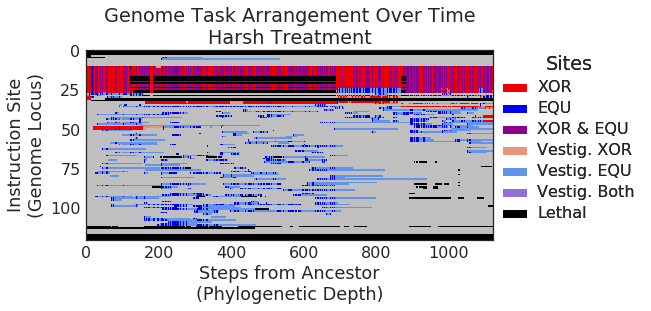
\includegraphics[width=0.5\columnwidth,trim={-0.82cm 0 5.2cm 0},clip]{figures/CE/harsh__whole_taskmap.png}}
% 	\caption{\textbf{Varying genetic architecture of \texttt{XOR} and \texttt{EQU} over time} for the final dominant genotype in a randomly selected replicate. Proceeding from the left of each figure, each vertical slice represents an organism along the line-of-descent to the final dominant.
% 	Positions along the Y-axis represent each genome locus; loci in an organism are colored based on the tasks that they code for. Sites in \textbf{red} are active sites that code for the \texttt{XOR} task only, sites in \textbf{blue} are active sites for the \texttt{EQU} task only, and \textbf{purple} sites code for both \texttt{XOR} and \texttt{EQU}. Knockouts to the sites in black are lethal to the organism. Sites in the lighter colors (tan, light blue, lavender) represent vestigial sites for \texttt{XOR} only, \texttt{EQU} only, or both tasks, respectively. As we proceed from left to right, we can see the evolutionary history of the final dominant genotype.}
% 	\label{fig:lineage}
% 	\end{figure}

	\begin{figure}[!h]
	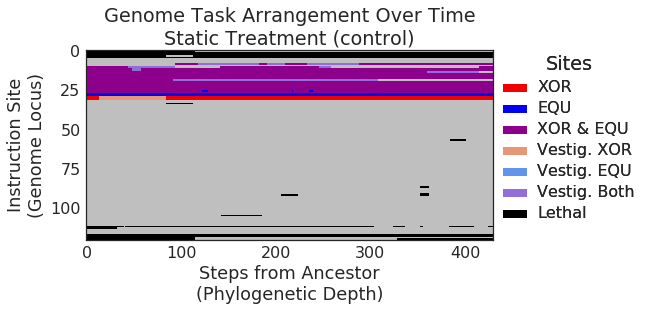
\includegraphics[width=0.75\columnwidth]{figures/CE/control__whole_taskmap.png}
	\caption{\textbf{Genetic architecture of \texttt{XOR} and \texttt{EQU} over time in static environment} for the final dominant genotype in a randomly selected replicate. Proceeding from the left of each figure, each vertical slice represents an organism along the line-of-descent to the final dominant.
	Positions along the Y-axis represent each genome locus; loci in an organism are colored based on the tasks that they code for. Sites in \textbf{red} are active sites that code for the \texttt{XOR} task only, sites in \textbf{blue} are active sites for the \texttt{EQU} task only, and \textbf{purple} sites code for both \texttt{XOR} and \texttt{EQU}. Knockouts to the sites in black are lethal to the organism. Sites in the lighter colors (tan, light blue, lavender) represent vestigial sites for \texttt{XOR} only, \texttt{EQU} only, or both tasks, respectively. As we proceed from left to right, we can see the evolutionary history of the final dominant genotype. \texttt{XOR} and \texttt{EQU} overlap almost completely throughout the run.}
	\label{fig:lineage-control}
	\end{figure}

	\begin{figure}[!h]
	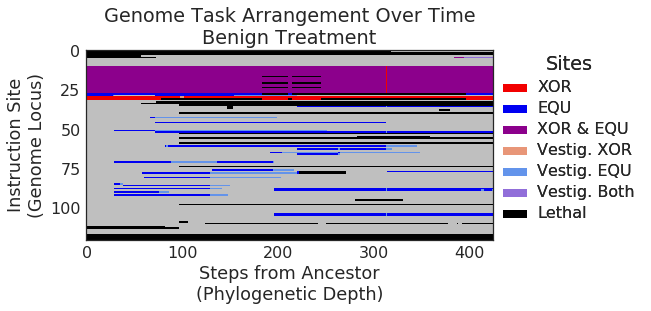
\includegraphics[width=0.75\columnwidth]{figures/CE/benign__whole_taskmap.png}
	\caption{\textbf{Genetic architecture of \texttt{XOR} and \texttt{EQU} over time in benign environment} for the final dominant genotype in a randomly selected replicate. Proceeding from the left of each figure, each vertical slice represents an organism along the line-of-descent to the final dominant, and as in Figure~\ref{fig:lineage-control}, colors represent tasks performed by each genome locus. In this genome, \texttt{XOR} and \texttt{EQU} evolve to overlap much less than in the control.}
	\label{fig:lineage-benign}
	\end{figure}

	\begin{figure}[!h]
	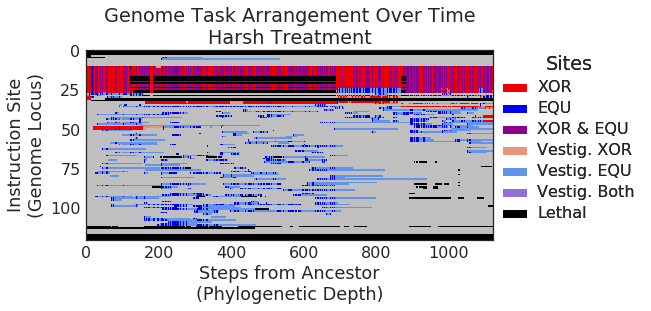
\includegraphics[width=0.75\columnwidth]{figures/CE/harsh__whole_taskmap.png}
	\caption{\textbf{Genetic architecture of \texttt{XOR} and \texttt{EQU} over time in harsh environment} for the final dominant genotype in a randomly selected replicate. Proceeding from the left of each figure, each vertical slice represents an organism along the line-of-descent to the final dominant, and as in Figures~\ref{fig:lineage-control} and \ref{fig:lineage-benign}, colors represent tasks performed by each genome locus. In this genome, \texttt{XOR} and \texttt{EQU} evolve to overlap even less than in the control and benign treatments, with the \texttt{EQU}-only task sites becoming increasingly scattered throughout the genome.}
	\label{fig:lineage-harsh}
	\end{figure}

%=arch of control, scattered XOR
In terms of site placement over time, functional task site locations in the control treatment did not change substantially over the course of the experiment. In the benign treatment, many more regions that performed the fluctuating task (XOR) were scattered throughout the genome, but site positions remained relatively fixed throughout the run after an initial adaptive phase. In the harsh treatment, however, not only are the active sites scattered, but the positions of active sites change and proliferate wildly over time.

%=site length
In addition to the variation in site placement, populations in the benign and harsh changing environment treatments had significantly more functional sites devoted to performing just the \texttt{EQU} task (Wilcoxon Rank Sum Test: Z = -5.57 and -6.96, respectively, p $<<$ 0.001).
%=reservoir of vestigial sites
Interestingly, populations evolved in both the benign and harsh treatments also show development of a large reservoir of formerly functional, now vestigial, sites; that is, sites that remain unchanged from when they were previously active in performing a task, but were disabled by a mutation elsewhere and are thus now neutral. These vestigial pseudogene-like sites may be important for allowing the organisms to quickly re-adapt as the fluctuations in the environment restore the previously-rewarded functions. (Fig~\ref{fig:CCE_func_vestigial})

%=[FIGURE - functional vs vestigial sites]
	\begin{figure}[!h]
	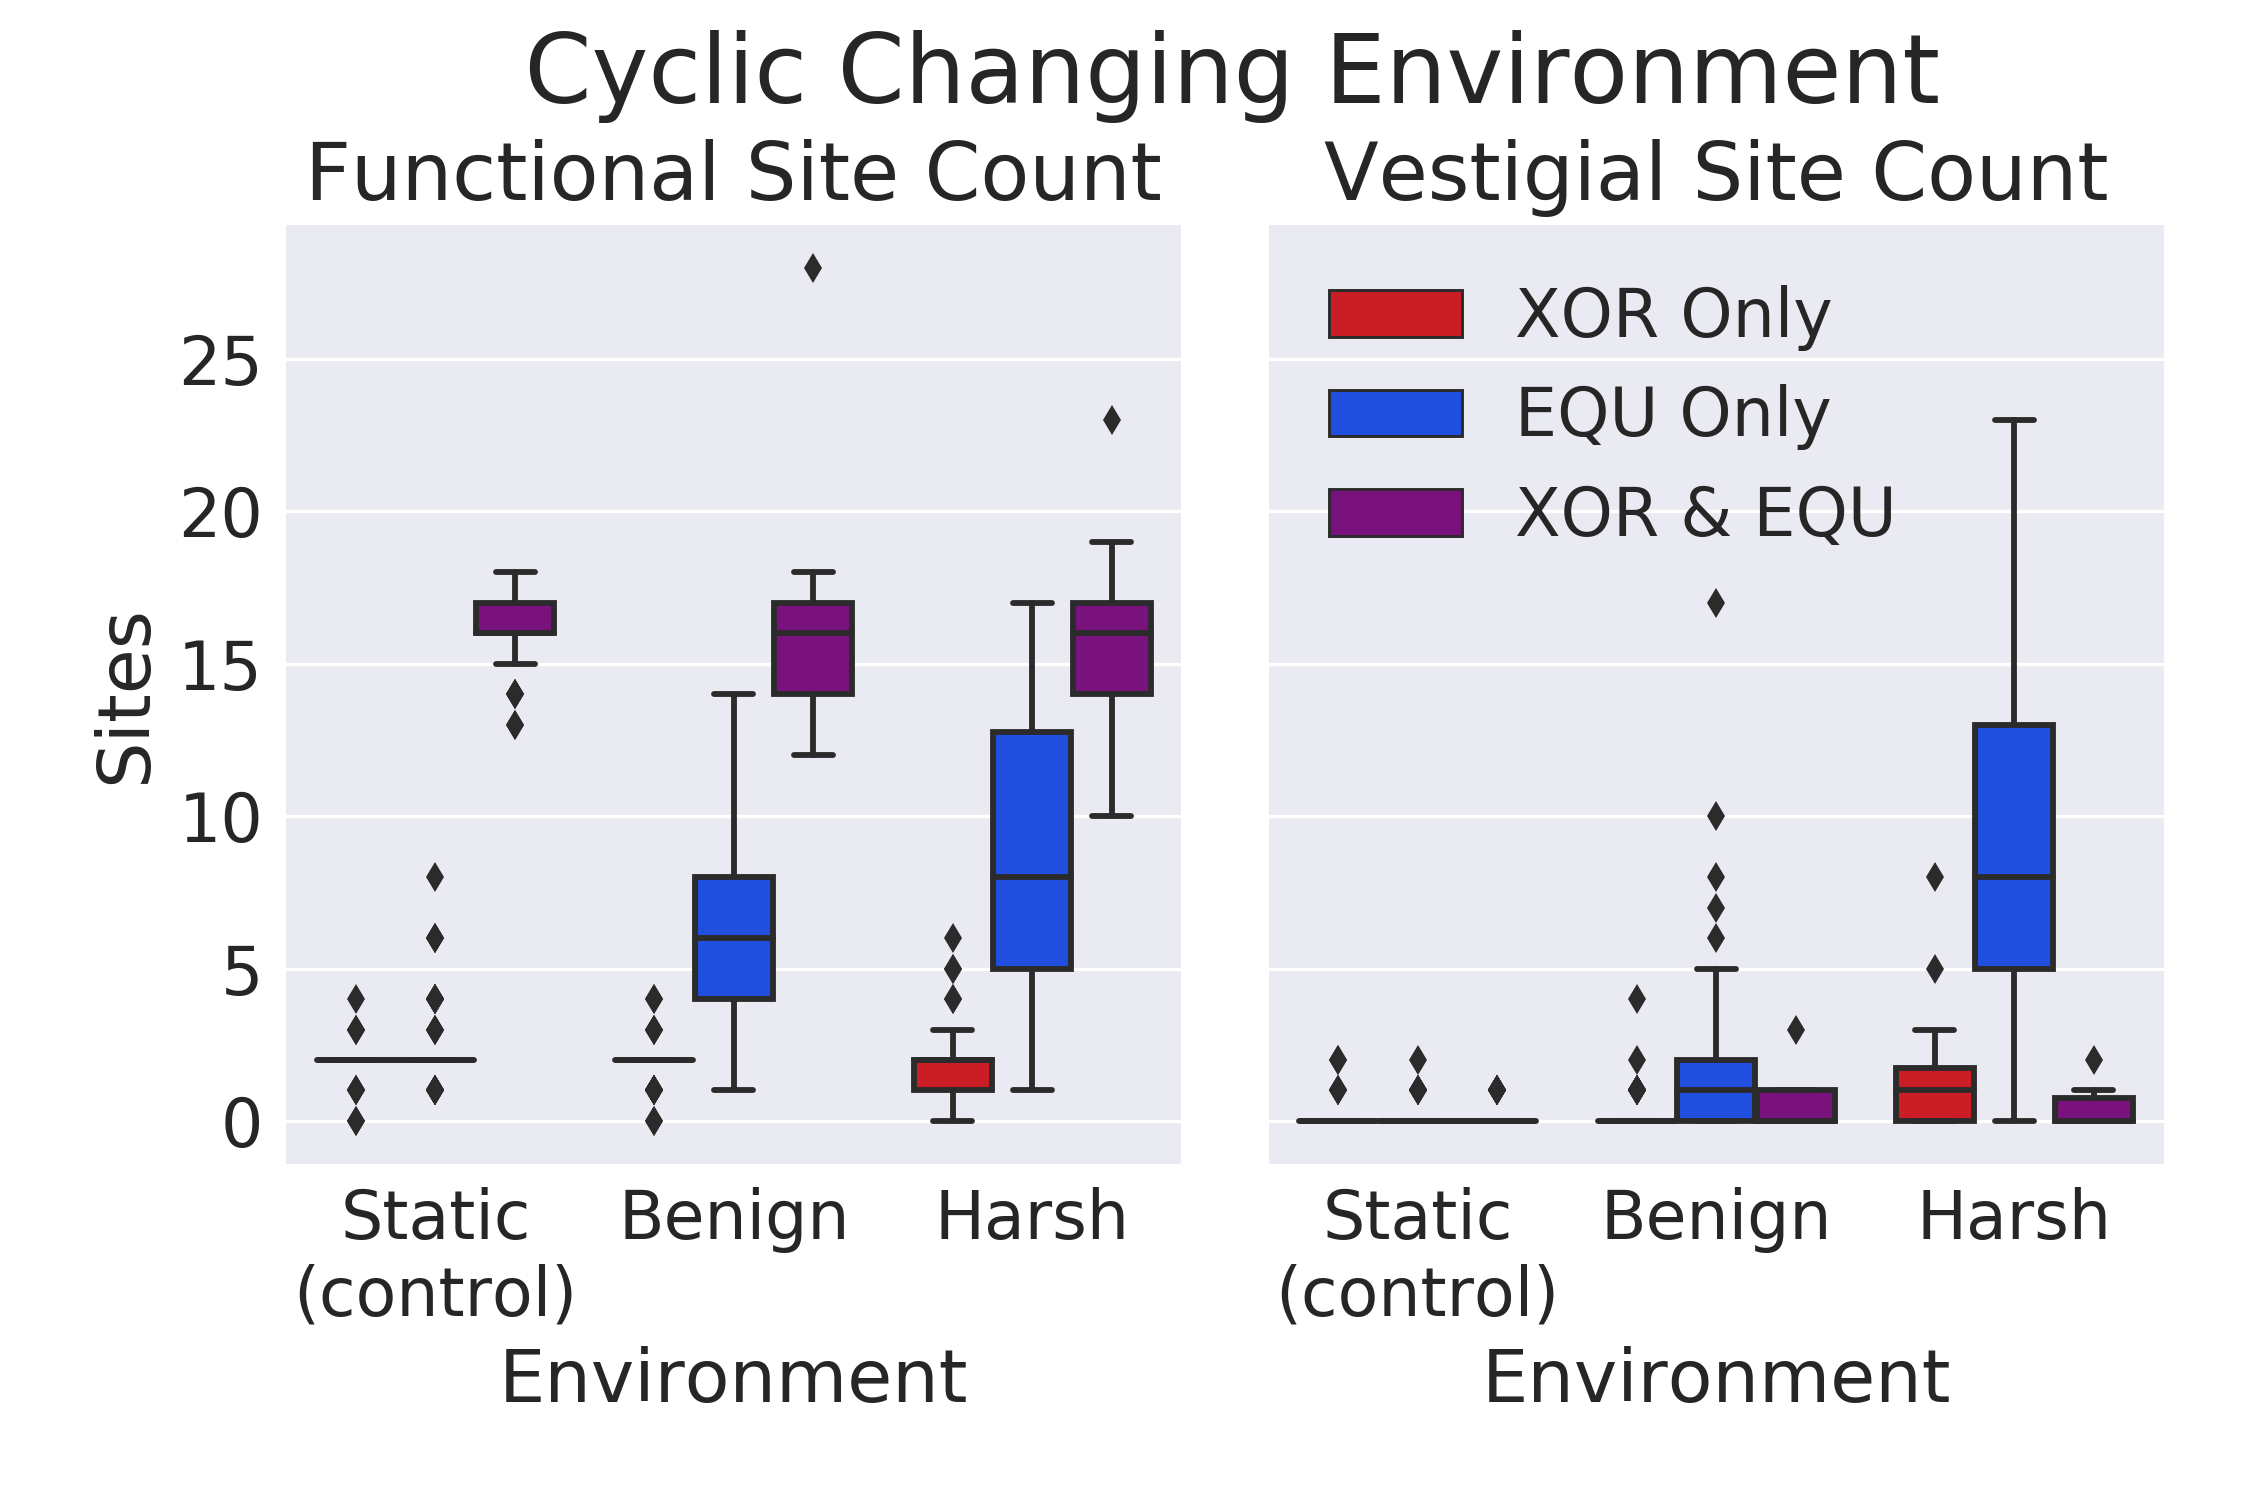
\includegraphics[trim={0 0 0 0}, clip, width=0.75\columnwidth]{figures/CE/CCE_func_vest__box.png}
	\caption{\textbf{Number of functional and vestigial sites by treatment}. Both the benign and harsh changing environments had significantly more sites devoted to performing only the \texttt{EQU} function (Wilcoxon Rank Sum Test: Z = -5.57 and -6.96, respectively, p $<<$ 0.001). The harsh environment has a significantly larger number of vestigial sites for the fluctuating (EQU) task compared to the benign treatment or control (Wilcoxon Rank-Sum Z = -6.57 and -8.33, p $<<$ 0.0001).
	}
	\label{fig:CCE_func_vestigial} %% FIGURE 5
	\end{figure}

\subsubsection*{Nearby Mutational Landscape}
%\todo[inline, color=yellow]{IF I HAVE TIME, add figure of the nearby landscape showing how mutations relate 1 and 2 steps out., a couple of nice figures showing both changes in detrimental mutations and phenotypic distribution.}

%=one-step survey of the mutational landscape 
In order to identify the role that these longer task footprints and pseudogene-like structures play, we performed a survey of the single-step mutational neighborhood surrounding the most abundant genotype present at the end of the experiment for each replicate population. Each neighborhood contained 3,025 distinct mutants (121 loci with 25 possible mutations per locus) in each of the 50 replicates per treatment, for a total of nearly 450,000 mutants surveyed. We measured the fraction of mutants that lost each of the rewarded tasks. (Fig~\ref{fig:CCE_single_step}). 

%=[FIGURE - Frac 1-step]
	\begin{figure}[!h] %% FIGURE 6
	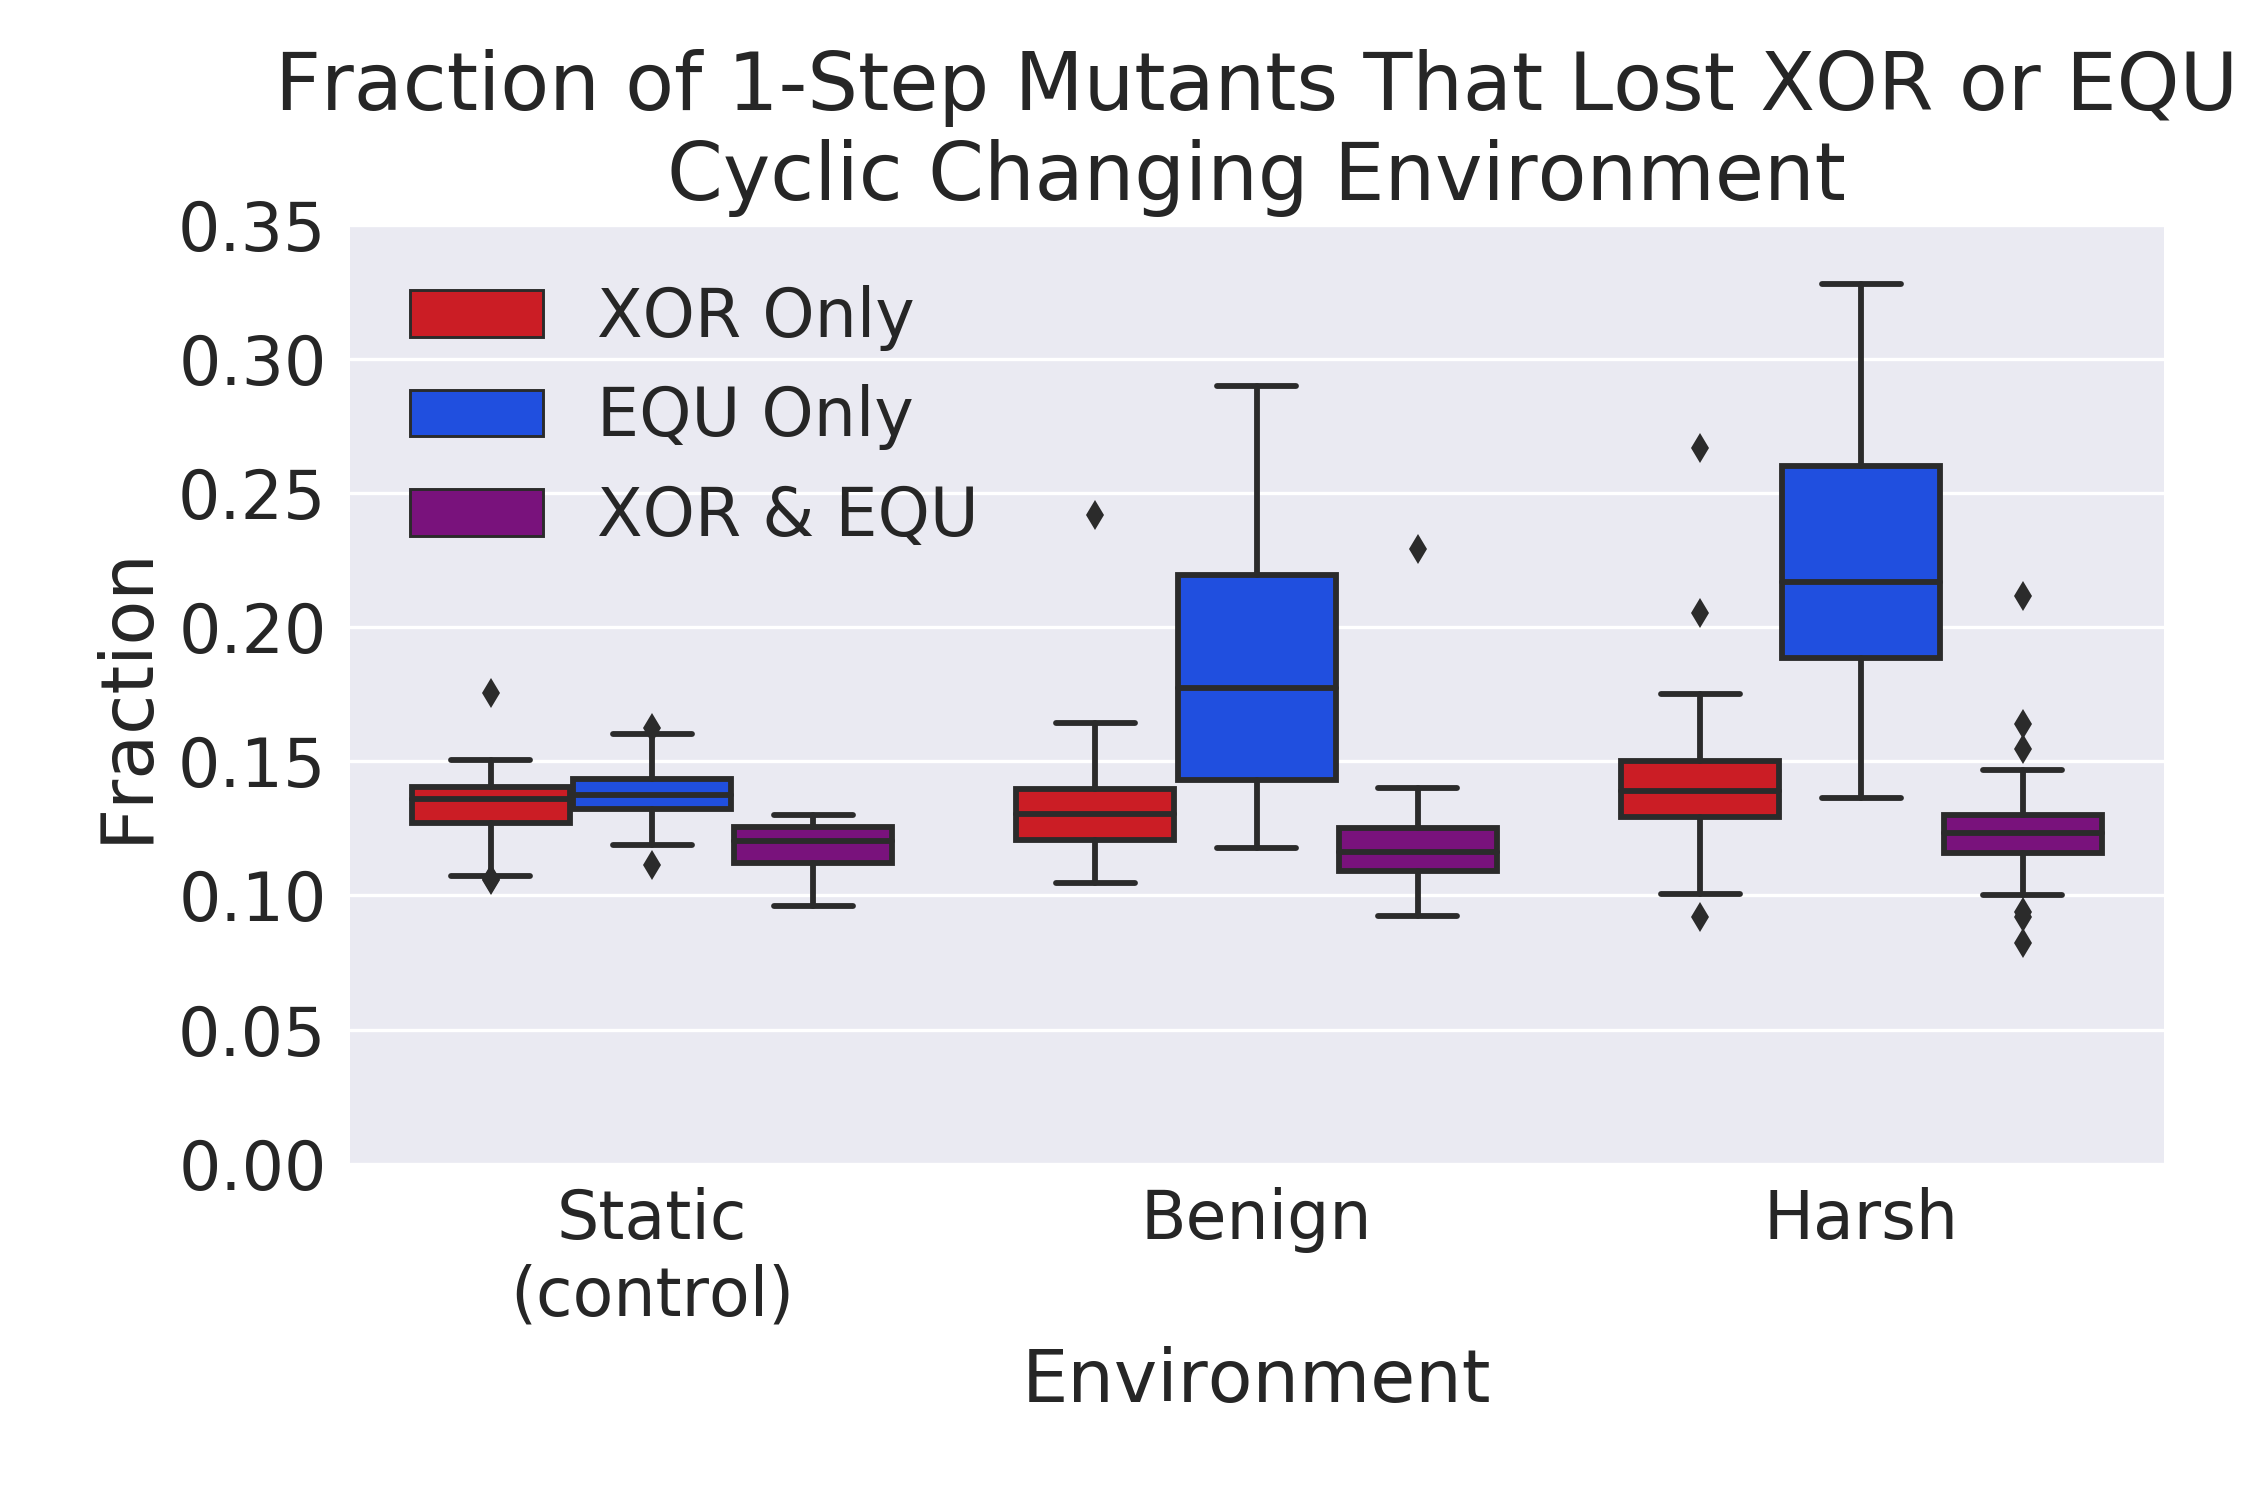
\includegraphics[trim={0.2cm 0 0 0.2cm},clip,width=0.75\columnwidth]{figures/CE/CCE_frac_1step__box.png}
	\caption{\textbf{A survey of the single-step mutational neighborhood} around organisms that performed the fluctuating task. Note that in both the benign and harsh treatments, there were significantly more mutants that lost the \texttt{EQU} task as compared to the control (Wilcoxon Rank Sum Test: Z = -5.46 and -7.80 respectively, p $<<$ 0.001). This result indicates that it was easier for the organisms in both treatments to turn off the \texttt{EQU} task in response to one mutation. 
	}\label{fig:CCE_single_step}
	\end{figure}


We found that in both the benign and harsh treatments, there were many more mutations that resulted in loss of the fluctuating task as compared to the control (Wilcoxon Rank Sum Test: Z = -5.46 and -7.80 respectively, p $<<$ 0.001). An increase in task loss in the harsh treatment is to be expected, but why would the benign treatment lose \texttt{EQU} nearly as easily as the harsh treatment? One possibility is selective pressure to lose the task. There is no explicit pressure for task loss, merely an absence of reward. Even so, there is certainly an implicit penalty for performing a complex task for which there is no reward. Another possibility is drift. Indeed, in Figure~\ref{fig:CCE_equ_execution}, we observe a steady downward trend in execution of \texttt{EQU} when rewards are withdrawn. Then, as the reward returns, new mutations are applied that reactivate the task, and overall performance recovers quickly. This pattern of loss and regain would, over time tend, to increase the length of the task. Indeed, as noted in Figure~\ref{fig:lineage-harsh}, there is a rapid increase in task length as \texttt{EQU} is cyclically lost and regained. 

\todo[inline]{make this a linear model, not just a correlation}
However, is increased task length enough to account for increased task vulnerability to mutation? In order to begin to address this question, we calculated the correlation between task length and the fraction of mutants that lost each of the tasks. We discovered a strong correlation between the number of functional sites and the number of task-losing mutants for the \texttt{EQU} task, both alone, and overlapping with \texttt{XOR} (Spearman's Rho: $r_s$ = 8.72 and 6.45, respectively, p = $<<$ 0.001) (Fig~\ref{fig:CCE_func_vs_single_step}). We also found a weaker, but still significant correlation between the number of \texttt{XOR}-only functional sites and loss of the \texttt{XOR} task (Spearman's Rho: $r_s$ = 3.85, p $<<$ 0.001). This result confirms our intuition that the longer the task, the more targets there are for mutation to disable the task.

%=[FIGURE - Frac 1-step vs task length]
	\begin{figure}[!h] %% FIGURE 6
	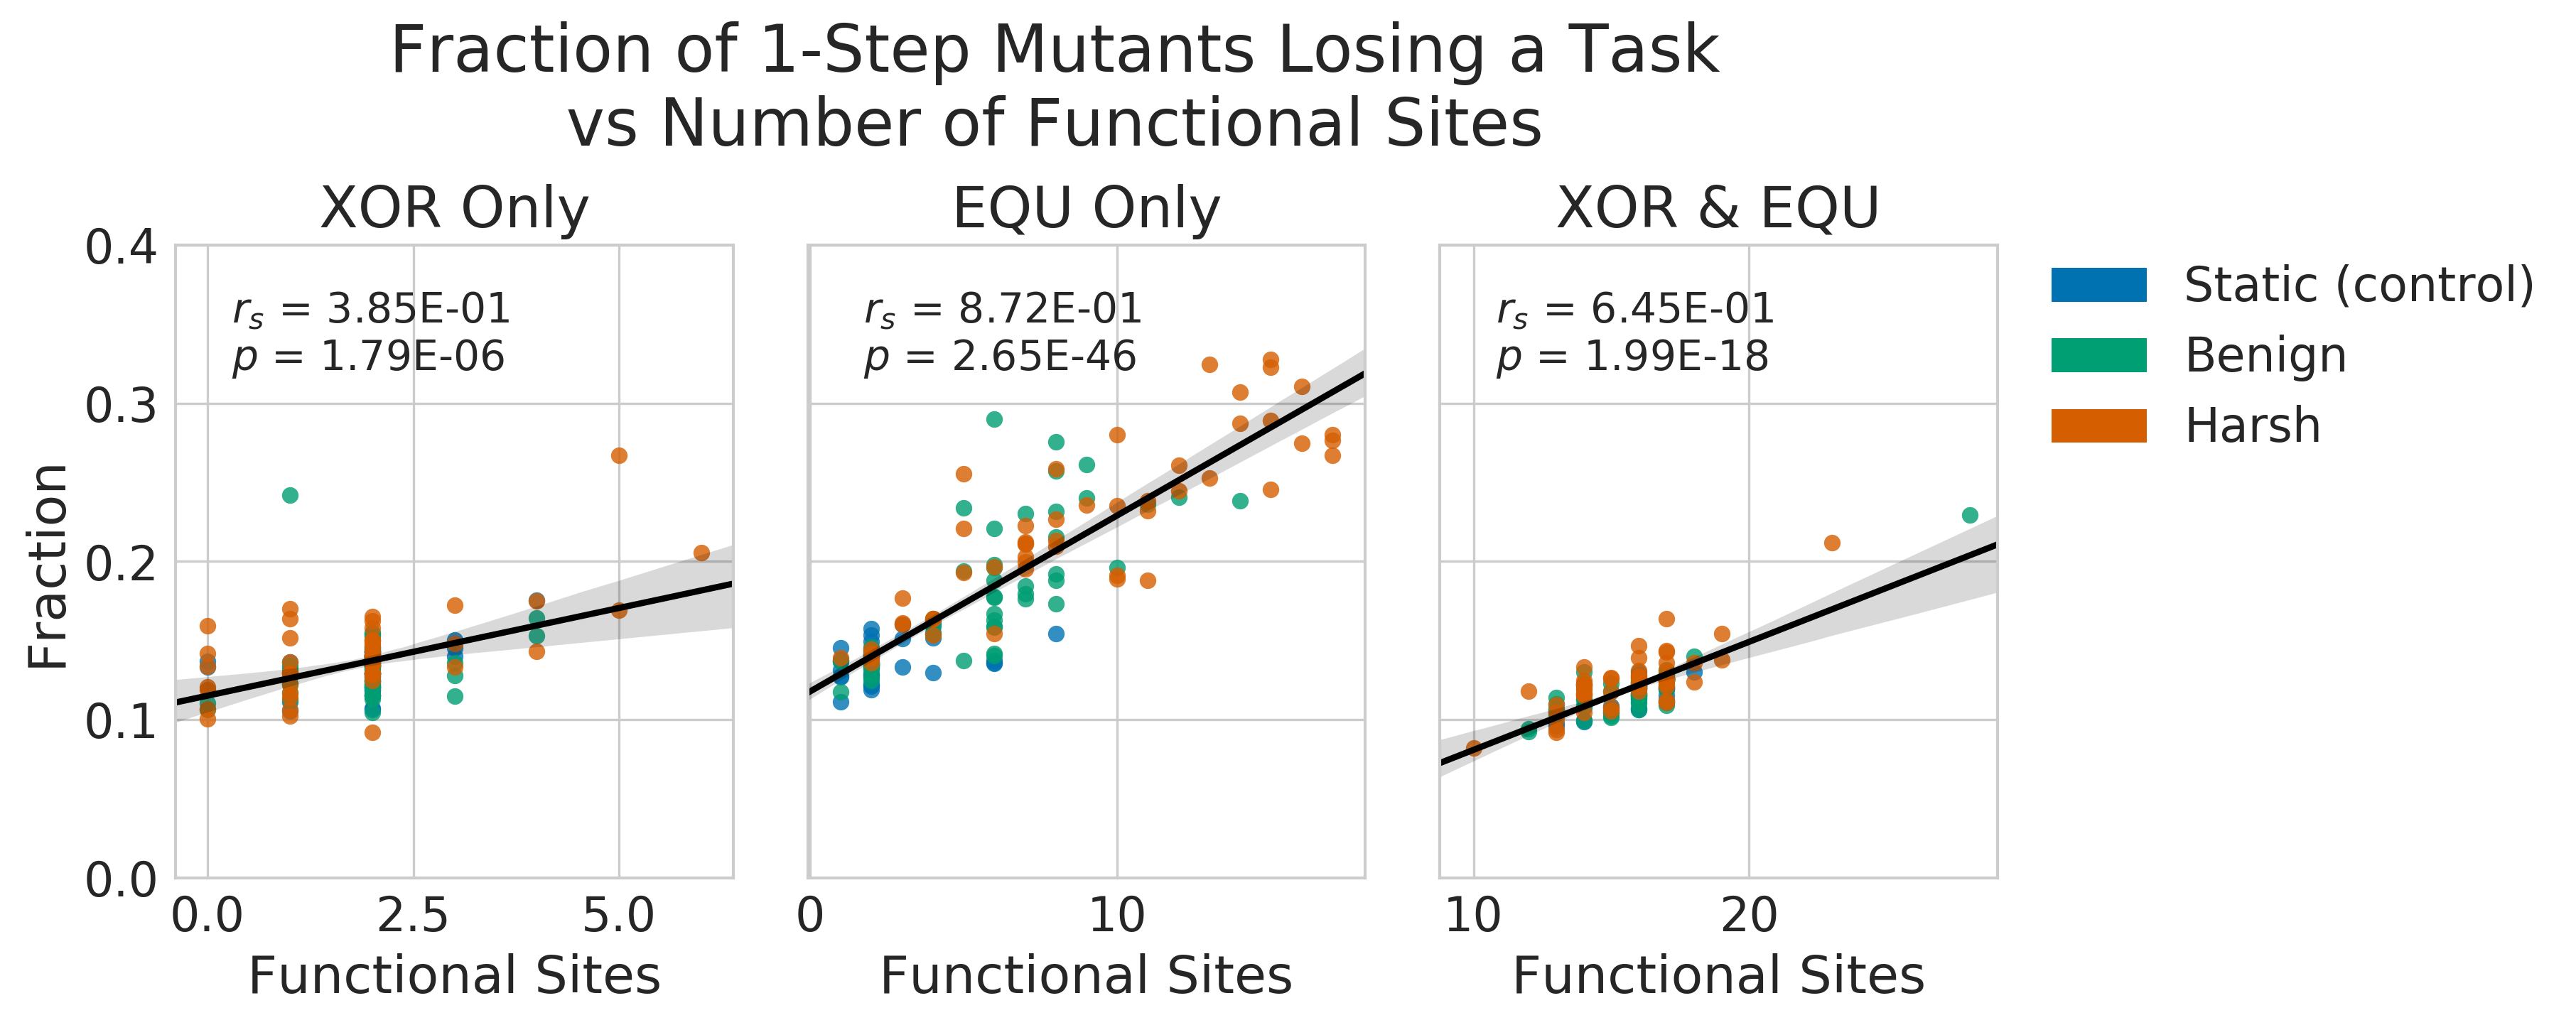
\includegraphics[trim={0.2cm 0 0 0.2cm},clip,width=0.95\columnwidth]{figures/CE/CCE_frac_1step_vs_func_sites.png}
	\caption{\textbf{Correlation between task length and mutational task loss} in the 1-step neighborhood across all treatments. Note the strong correlation between the length of the \texttt{EQU} task and the fraction of mutants that lost \texttt{EQU} (Spearman's Rho: $r_s$ = 8.72, p $<<$ 0.001). Further, consider the weaker correlation between \texttt{XOR} task length, and fraction of mutants that lost \texttt{XOR}. This suggests that \texttt{EQU} is even less robust to mutation compared to \texttt{XOR} than can be accounted for by task length alone.  
	}\label{fig:CCE_func_vs_single_step}
	\end{figure}	
% @CAO: I also get why we should expect to see \texttt{EQU} lost easily in the Harsh changing environment, but why is it also lost so easily in the benign environment. Should we speculate here?  (Or do you below?)  More generally, why do you think this is the case?
% @CAO: One other thought for how this result may happen. Maybe in the control there is a pressure for \texttt{EQU} to evolve to be more robust, whereas the changing environment just doesn't give it time to evolve robustness. I can't think of a way to easily disentangle those explanations though...
% @RCK: clarify that benign are lost due to drift.
% @RCK - NOTE TO SELF -- see about joining vestigial sites paper with Matt's bias work. Are vestigial sites useful because they are random building blocks available (equivalent to mutational bias), or is there a deeper functional structure. Does order matter?
% @RCK: Performed a correlation between task length and task loss, and find a strong correlation. Because the \texttt{EQU} task is longer is both the changing environments, it'll be lost more easily in both cases.

Further, the lower correlation between length and task loss for the \texttt{XOR} suggests that it is not only task length, but some other architectural feature that makes the \texttt{XOR} task more robust to mutation, and the \texttt{EQU} task more fragile. Even so, the question of what kinds of architectural features account for this differential robustness remains open.

We then measured the proportion of second step mutants that regained \texttt{EQU} after having lost it in the single-step survey. We found that 
%the availability of reservoirs of vestigial sites 
changing environments shifted
shifted the populations' position in the mutational landscape, such that when a task that was lost due to mutation, that task could be regained via one or two additional mutations elsewhere. That is, once a mutation caused the loss of a task, a different mutation could reactivate the task. (Fig~\ref{fig:CCE_two_step}). 
% @CAO: This last part doesn't make a lot of sense -- CLEARLY if a single mutation causes a task loss, the corresponding reverse mutation would cause that task to be regained. As such, do you mean that there a MORE paths back to the task in the changing-environment treatments as compared to the static control?
% @RCK: Yes, that's what this means. "More often, above". I can clarify. 
%@RCK: Clarified

%=[FIGURE - Frac 2-step]
%@CAO - I wonder if it would be interesting to list the number of ways that this happened to be clear that we're not just talking about undoing the changes that caused the loss in the first place.
%@RCK: just clarified that we're not talking about reversions. More explanation provided above.
	\begin{figure}[!h] %% FIGURE 7
	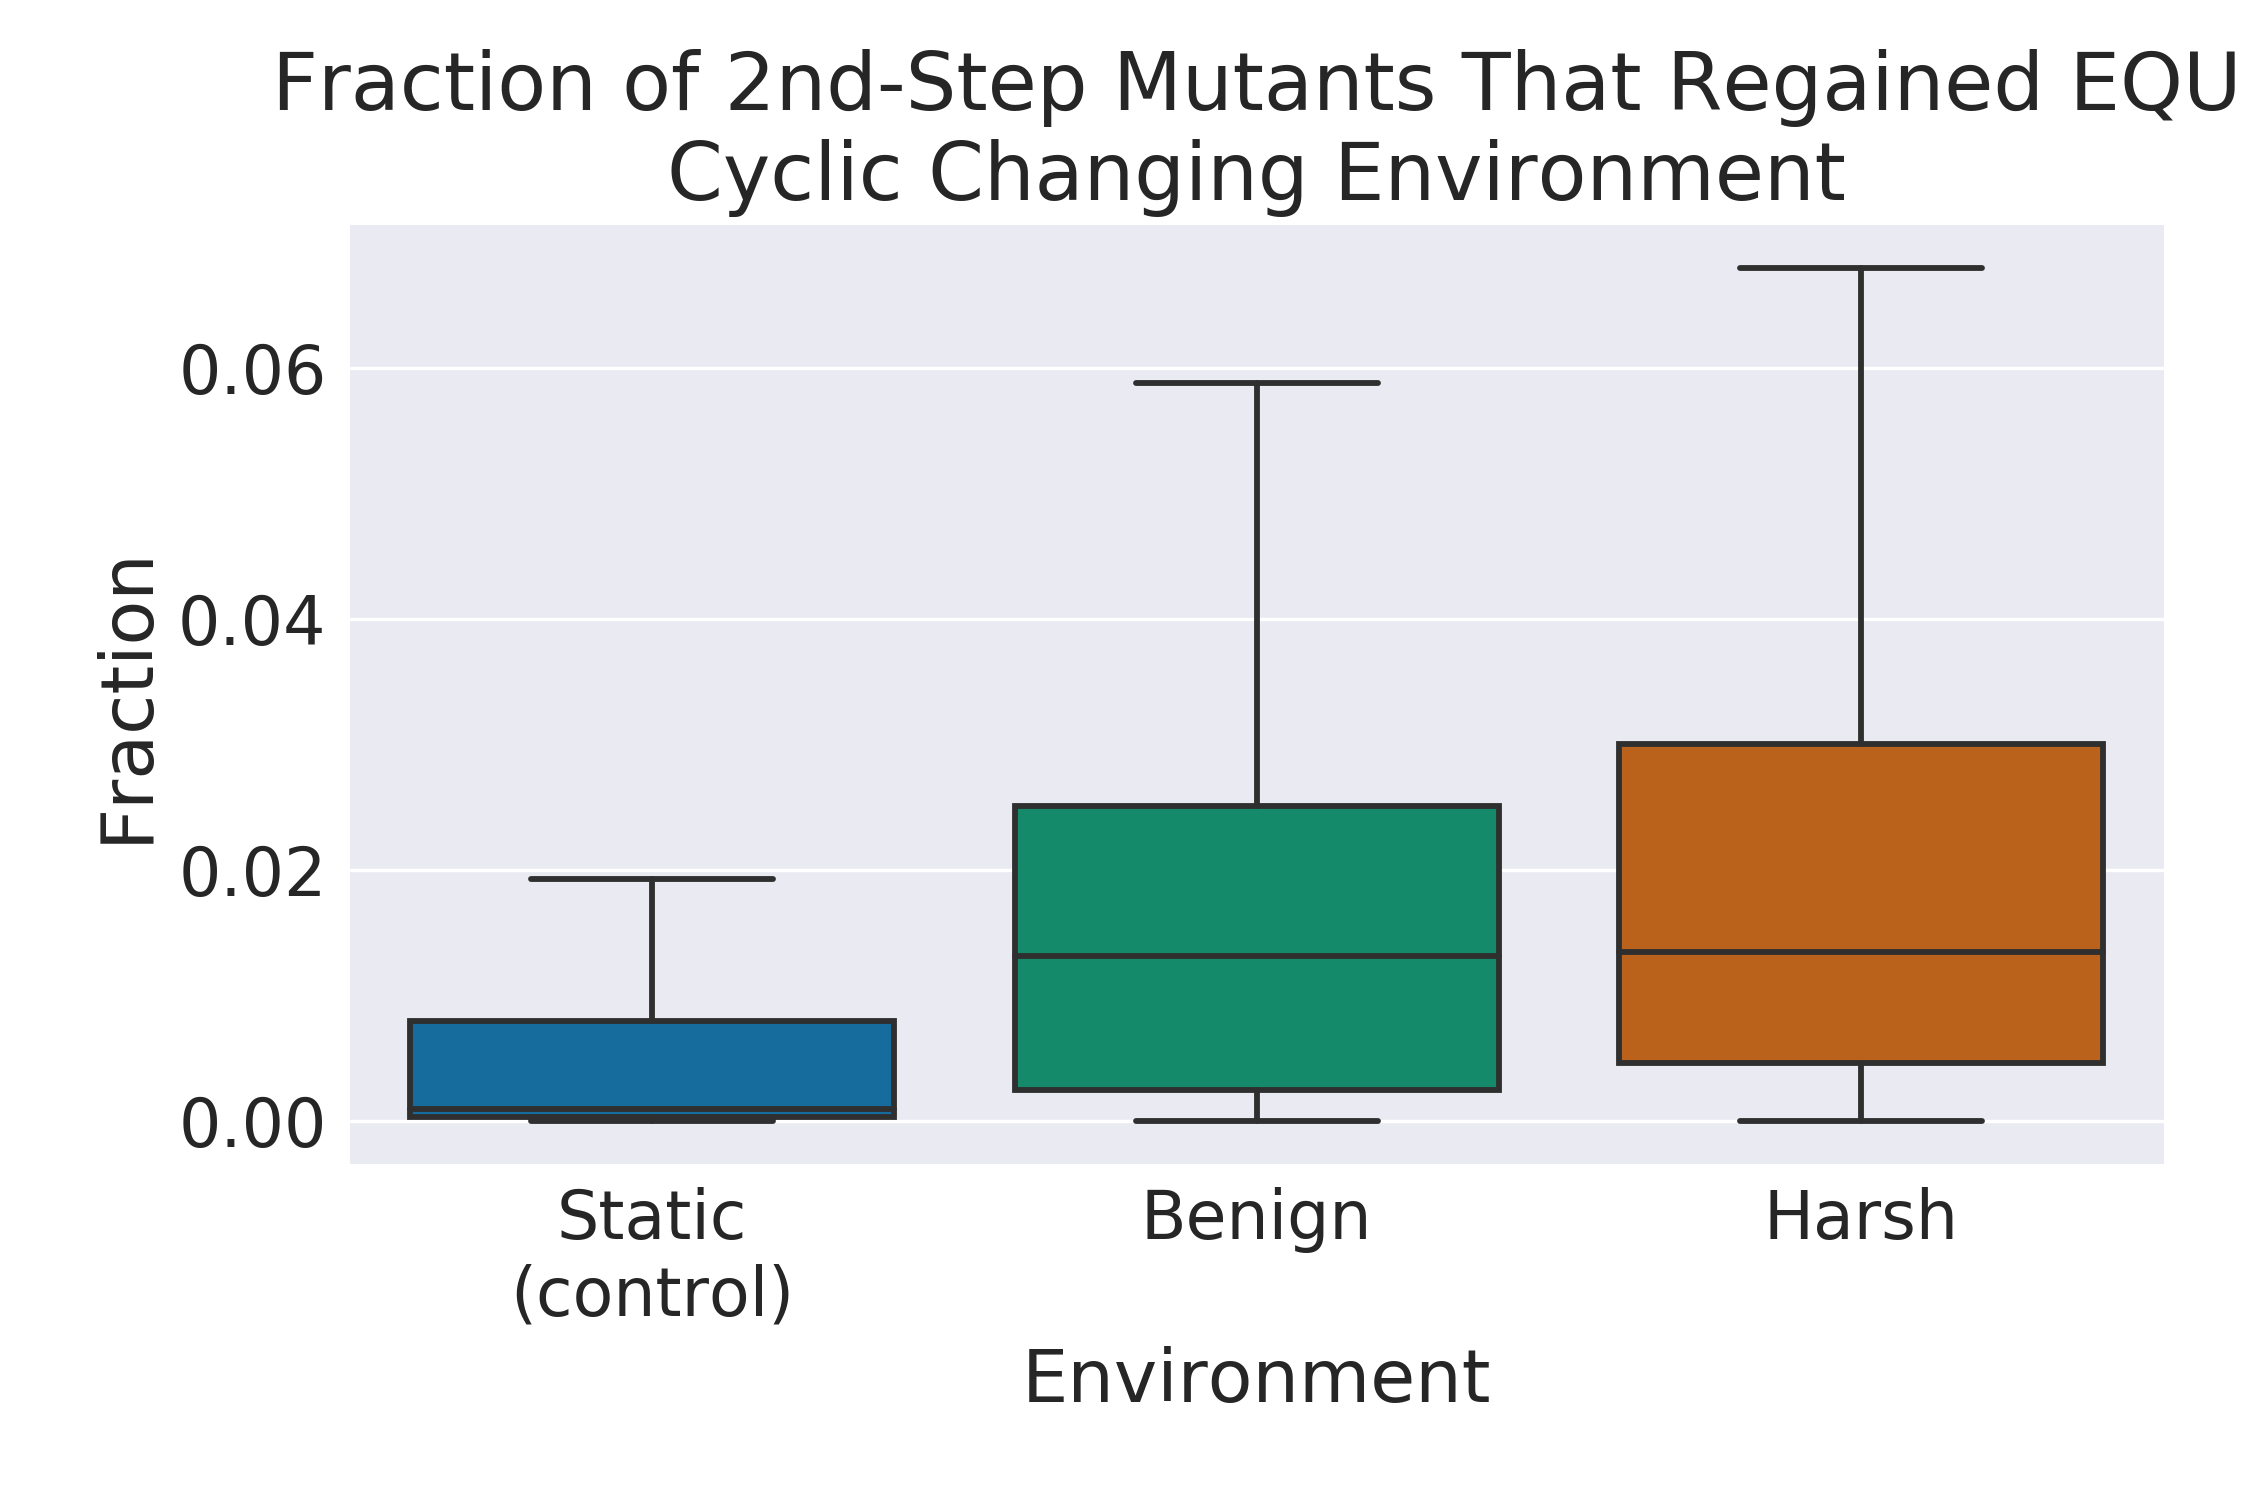
\includegraphics[width=0.75\columnwidth]{figures/CE/CCE_frac_2step__box.png}
	\caption{\textbf{A survey of the two-step mutational neighborhood} of the organisms that lost \texttt{EQU} function in the one-step survey. We found that in both the harsh and benign treatments, there were significantly more organisms that regained function in response to mutation than the control. (Wilcoxon Rank Sum Test: Z = -47.9 and -57.82 respectively, p $<<$ 0.0001). This result indicates that it was easier for the organisms in both fluctuating environments to regain the task in response to one additional, non-reversion mutation.   
	}\label{fig:CCE_two_step}
	\end{figure}

We speculate that this effect is due to the availability of reservoirs of formerly vestigial sites. How such reservoirs might perform these functions remains an open question. New mutations may either re-enable the old functional sites, or recruit vestigial functionality to perform the task elsewhere. Potentially, these vestigial sites are not altogether dormant at all. They might individually appear vestigial in the context of a single knockout survey, but they might also be related to other sites in a network of backup functionality that becomes activated in response to mutation. More research is needed to explore what role these feature play. 






%=measured D_g, D_p, found similarity in D_g, increase in D_p 
As an overall measure of neutral exploration, we also measured the proportion of non-deleterious mutants in the nearby fitness landscape - the Genomic Diffusion Rate. We found that this proportion remained approximately the same between all treatments (Kruskal-Wallis: H(2) = 1.44, p = 0.49). However, we found that the Phenotypic Diffusion Rate, the proportion of these mutants with different (and potentially adaptive) phenotypes, increased in the changing environment treatments as compared to the controls (Wilcoxon Rank Sum Test: Z = -8.02, -8.39, respectively, p $<<$ 0.001). In this way, the organisms from the changing environment treatments have an advantage over organisms from the control runs in the short-term evolvability of the fluctuating task. This result is consistent with real adaptation, not only to resources in their local environment, but a direct adaptation to the environmental change. (Fig~\ref{fig:CCE_diffusion_rate})

%=[FIGURE D_g D_p]
	\begin{figure}[!h] %% FIGURE 8
	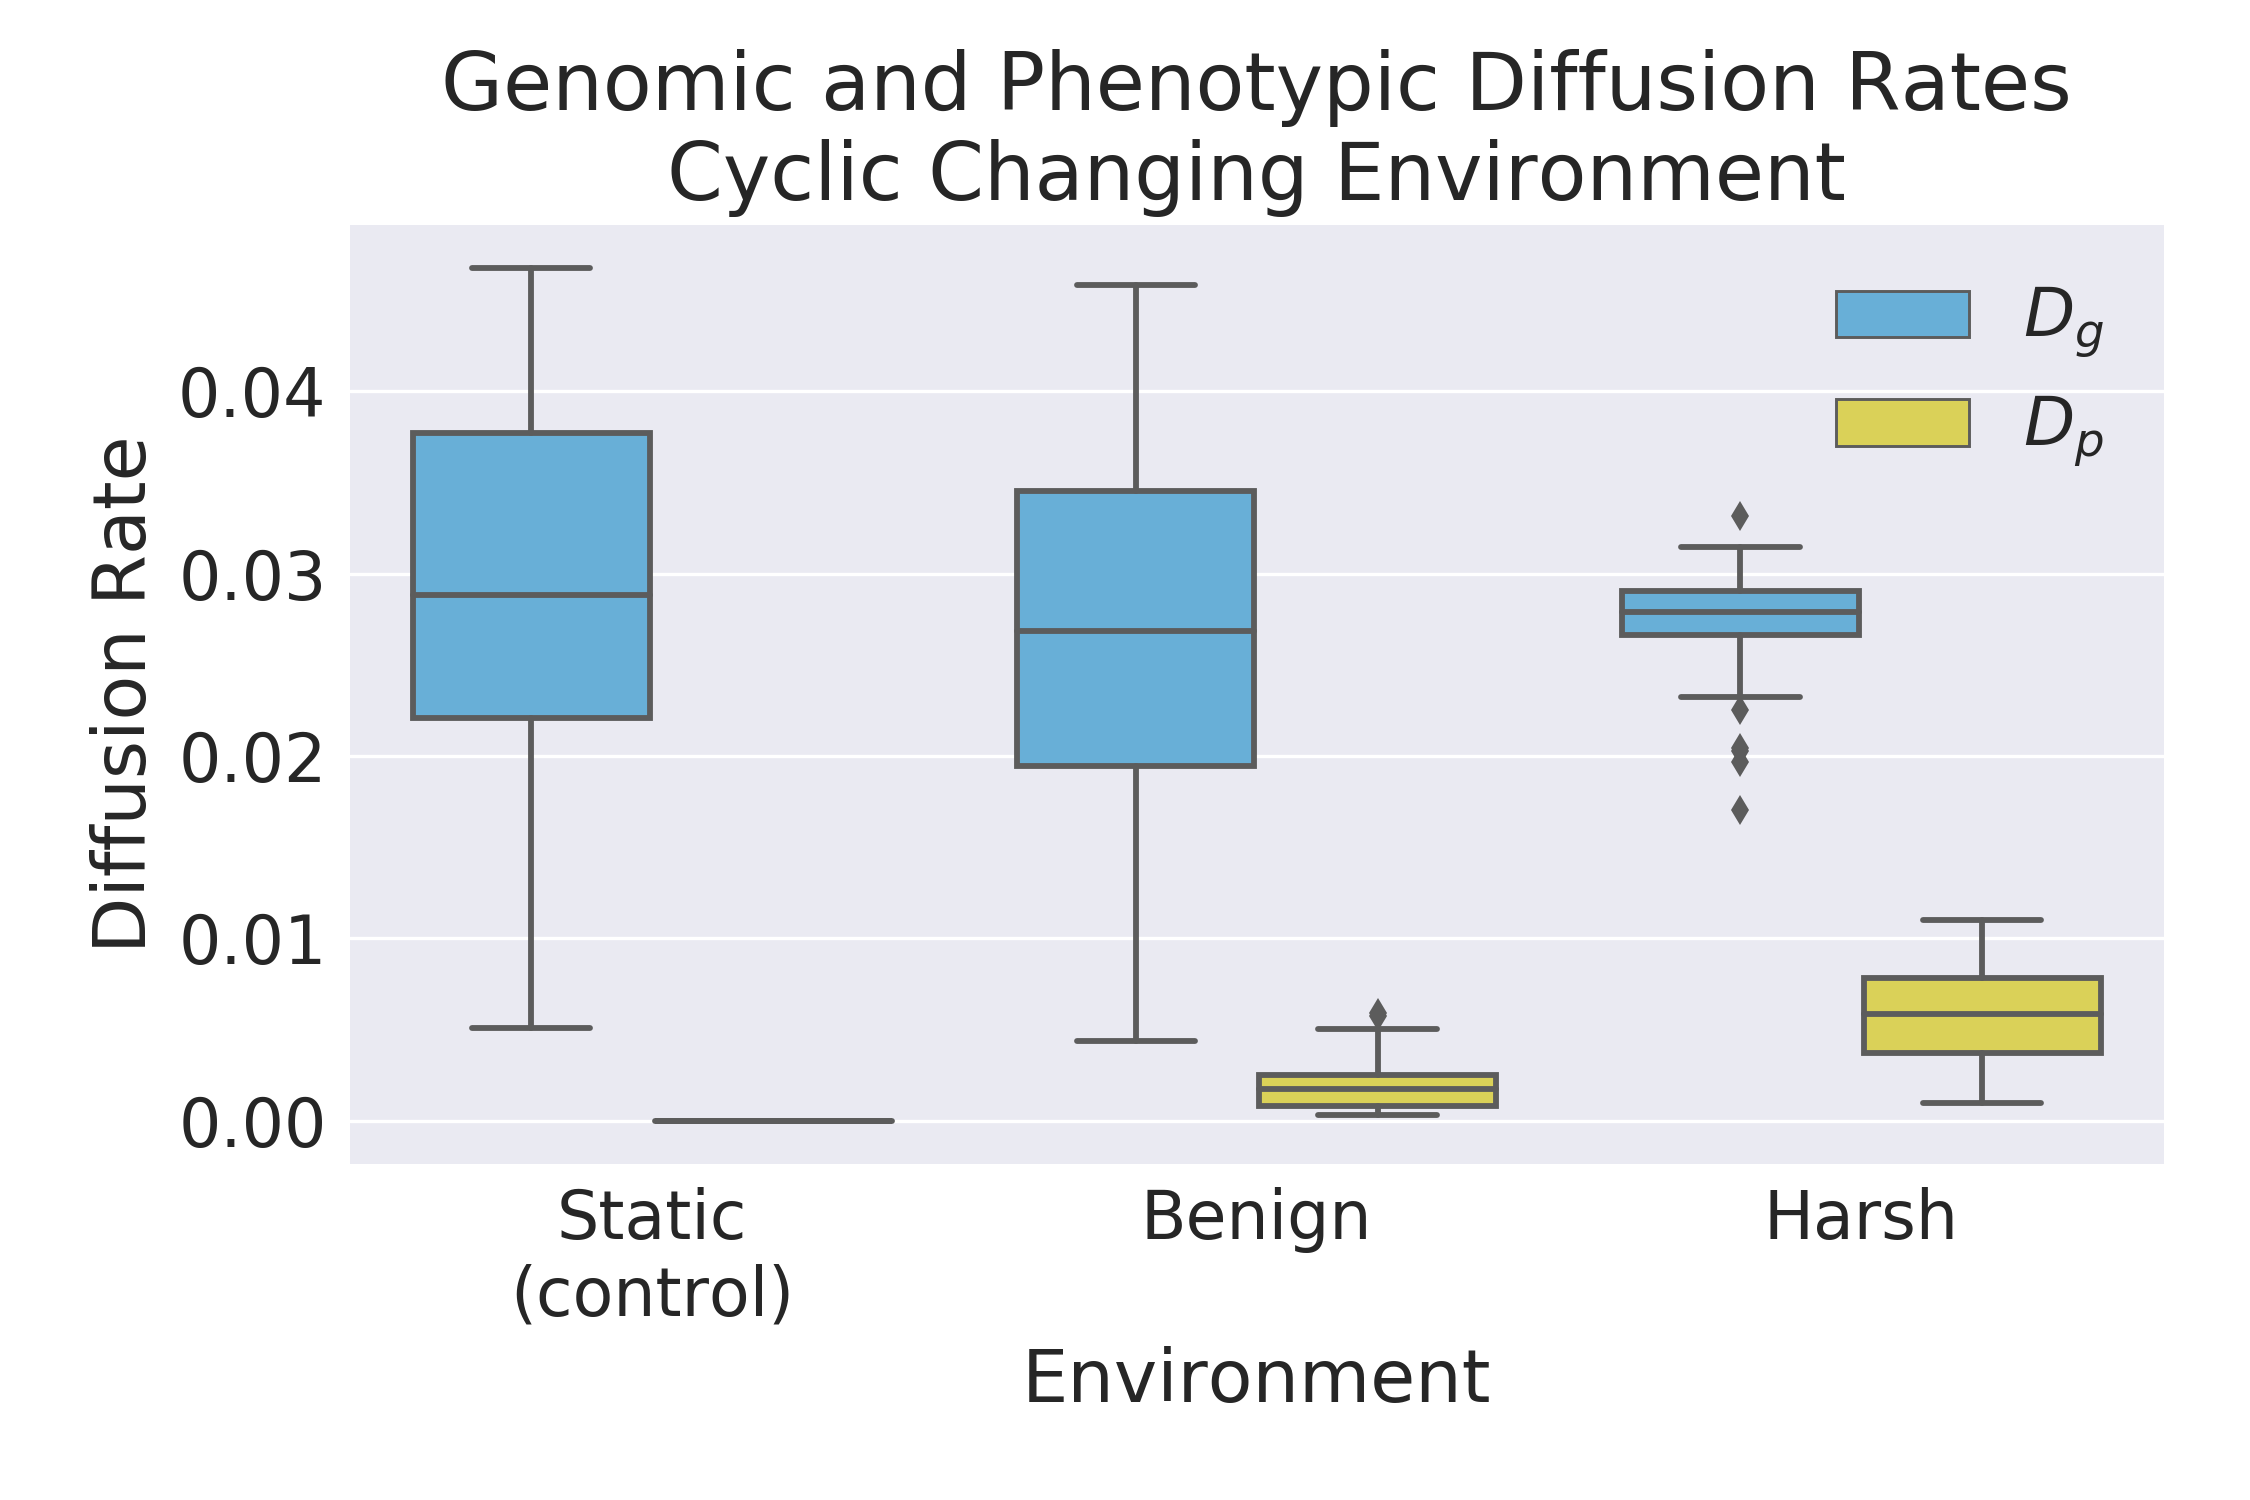
\includegraphics[width=0.75\columnwidth]{figures/CE/CCE_D_g_D_p__box.png}
	\caption{\textbf{Genomic and phenotypic diffusion rates}, showing the probabilities of producing offspring that are genotypically ($D_g$) or phenotypically ($D_p$) distinct from the parent, while not reducing fitness.
	Note that while overall neutral exploration capacity remains relatively stable between treatments (Kruskal-Wallis: H(2) = 1.44, p = 0.49), phenotypic exploration capacity is increased in both treatments, but especially in the Harsh treatment. (Wilcoxon Rank Sum Test: Z = -8.02, -8.39, respectively, p $<<$ 0.001). This result is consistent with changing environments promoting the phenotypic evolvability of populations.
	}\label{fig:CCE_diffusion_rate}
	\end{figure}

What might account for this adaptation? Similar to the relationship between the number of functional sites of a task, and the number of single-step mutants that lost that task (See Fig~\ref{fig:CCE_func_vs_single_step}), we hypothesize that the reacquisition of tasks in the 2nd-step survey may be mediated by the amount of useful task material present in the genome. We performed a multiple linear regression, predicting the mean fraction of mutants that regained \texttt{EQU}, by the number of functional and vestigial sites contained in the original genome (See Table~\ref{ce-olsregression-2ndstep} and Fig~\ref{fig:CCE_2step_vs_func_vest_sites}).

	%=[FIGURE 2nd-Step ~ Func + Vest]
	\begin{figure}[!h] %% FIGURE 8
	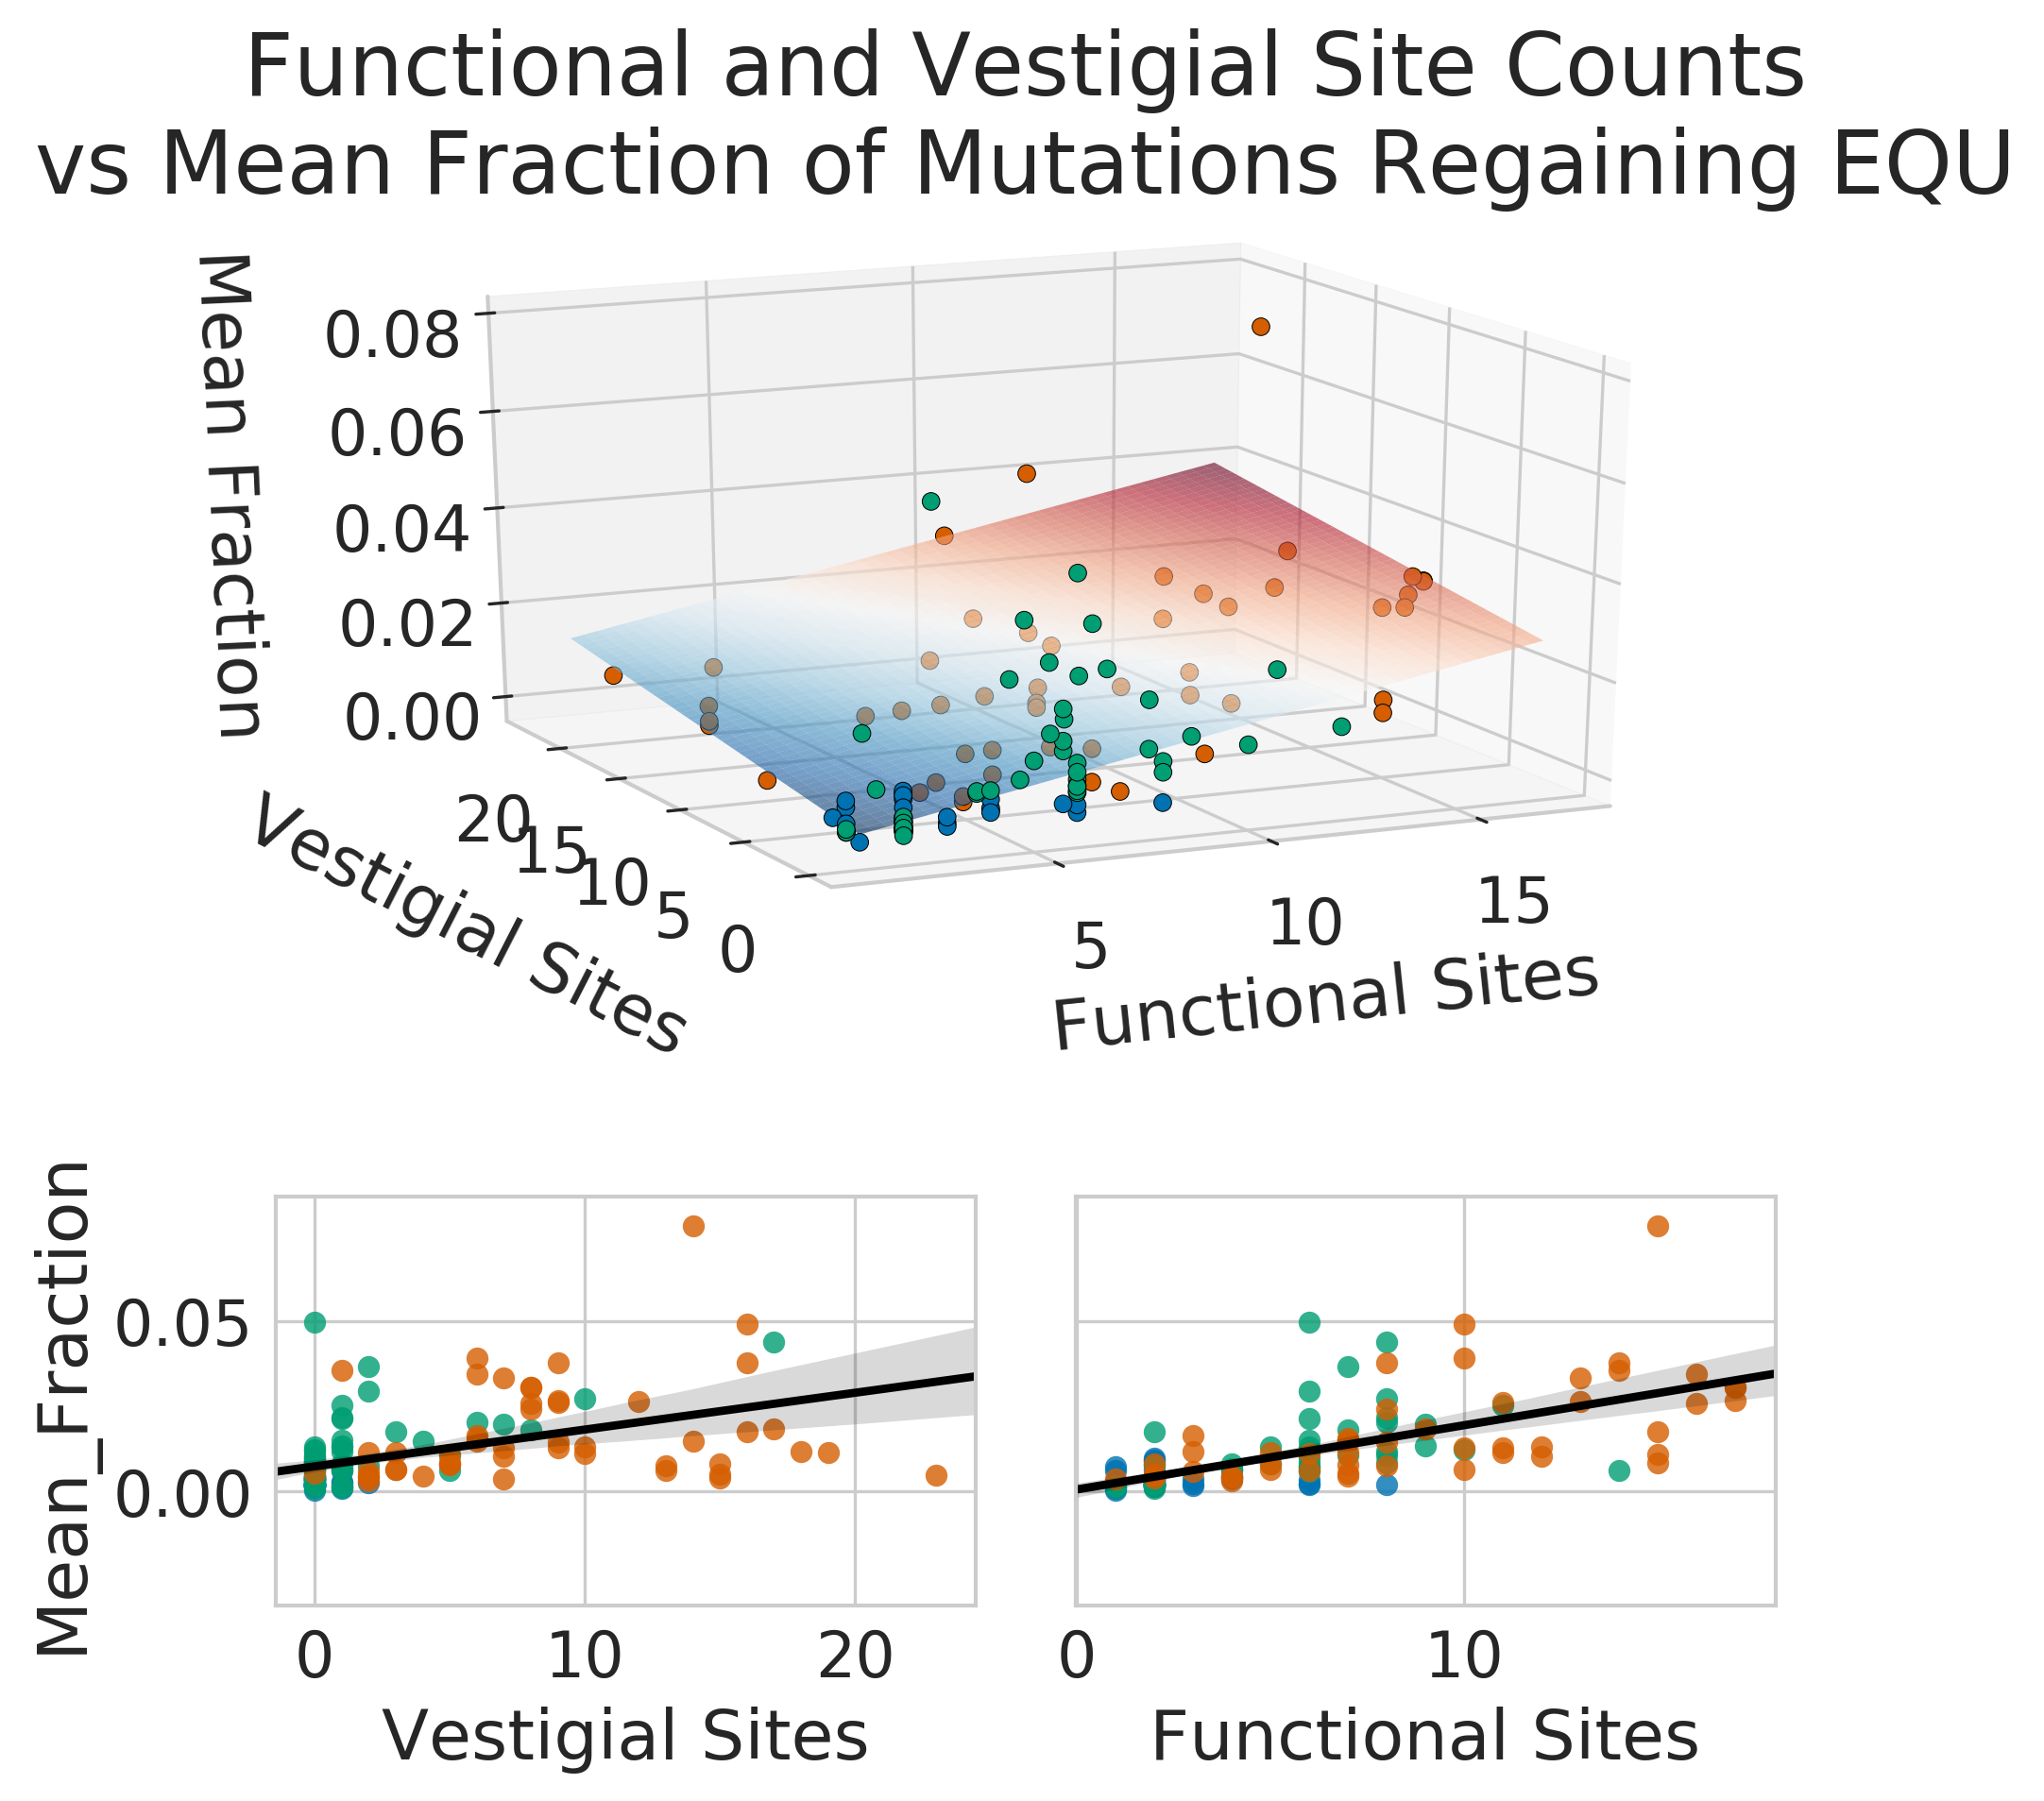
\includegraphics[width=0.75\columnwidth]{figures/CE/CCE_2step_vs_func_vest_sites.png}
	\caption{\textbf{Multiple linear regression predicting mean fraction of second-step mutants} from the number of functional and vestigial sites in the original organism. See Table~\ref{ce-olsregression-2ndstep}.
	}\label{fig:CCE_2step_vs_func_vest_sites}
	\end{figure}

We can predict approximately 47\% of the variation in mean number of second step mutants that regained \texttt{EQU} based on the number of functional and vestigial sites. Most of the variation is predicted by the number of functional sites, though vestigial sites do contribute a small amount. This result is consistent with the role of task length, and thus the number of informational sites, being important for regaining task function. We could not, however, account for all variation, indicating that there are other factors, possibly in robustness or modular architecture of tasks, that are important to this kind evolvability.

	\begin{table}[h]
	\centering
	\caption{\textbf{OLS Regression Results - Mean Fraction of Mutants Regained \texttt{EQU} vs Number of Functional and Vestigial Sites}}
	\label{ce-olsregression-2ndstep-h}
	\begin{tabular}{lclc}
	\toprule
	\textbf{Dep. Variable:}    &  Mean\_Fraction  & \textbf{  R-squared:         } &     0.472   \\
	\textbf{Model:}            &       OLS        & \textbf{  Adj. R-squared:    } &     0.464   \\
	\textbf{Method:}           &  Least Squares   & \textbf{  F-statistic:       } &     61.65   \\
	\textbf{No. Observations:} &         141      & \textbf{  Prob (F-statistic):} &  7.39e-20   \\
	\textbf{Df Residuals:}     &         138      & \textbf{  Log-Likelihood:    } &    467.28   \\
	\textbf{Df Model:}         &           2      & \textbf{  AIC:               } &    -928.6   \\
	                           &                  & \textbf{  BIC:               } &    -919.7   \\
	\bottomrule
	\end{tabular}
	\begin{tabular}{lcccccc}
	                     & \textbf{coef} & \textbf{std err} & \textbf{t} & \textbf{P$>$$|$t$|$} & \textbf{[0.025} & \textbf{0.975]}  \\
	\midrule
	\textbf{Intercept}   &       0.0003  &        0.001     &     0.243  &         0.808        &       -0.002    &        0.003     \\
	\textbf{Func\_Sites} &       0.0016  &        0.000     &     8.115  &         0.000        &        0.001    &        0.002     \\
	\textbf{Vest\_Sites} &       0.0005  &        0.000     &     3.180  &         0.002        &        0.000    &        0.001     \\
	\bottomrule
	\end{tabular}
	\begin{tabular}{lclc}
	\textbf{Omnibus:}       & 79.316 & \textbf{  Durbin-Watson:     } &    1.928  \\
	\textbf{Prob(Omnibus):} &  0.000 & \textbf{  Jarque-Bera (JB):  } &  437.211  \\
	\textbf{Skew:}          &  1.970 & \textbf{  Prob(JB):          } & 1.15e-95  \\
	\textbf{Kurtosis:}      & 10.675 & \textbf{  Cond. No.          } &     15.0  \\
	\bottomrule
	\end{tabular}
	\begin{flushleft}Multiple linear regression, predicting Mean fraction of second-step mutants that regained \texttt{EQU}, based on the number of Functional and Vestigial sites in the original genome.  
	\end{flushleft}
	\label{ce-olsregression-2ndstep}
	\end{table}


% \subsection*{Stochastic Changing Environments}
% %=[FIGURE - D_g/p]
% 	\begin{figure}[!h] %% FIGURE 12
% 	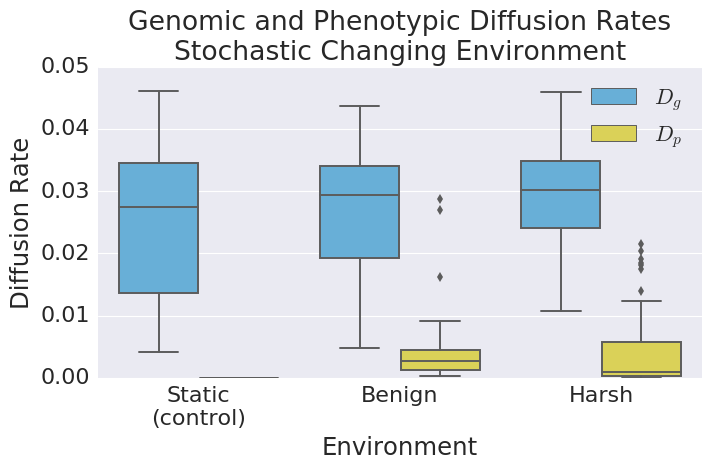
\includegraphics[width=0.75\columnwidth]{figures/CE/CSE_D_g_D_p__box.png}
% 	\caption{\textbf{Genomic and phenotypic diffusion rates} in stochastic changing environments, showing the probabilities of producing offspring that are genotypically and phenotypically different from the parent, while remaining fitness neutral or better. As in the cyclic environment, $D_g$ remains stable for the Benign treatment, but drops slightly in the Harsh as compared to the control, though this drop isn't statistically significant (Kruskal-Wallis H(2) = 1.11, p = 0.57). Harsh $D_p$ however, is significantly lower than seen in the cyclic environment treatment (Wilcoxon Rank-Sum Test: Z = -6.19, p $<<$ 0.0001). This result shows that harsh stochastic environments may not be as effective as cyclic environments at increasing the probability that organisms will produce phenotypically different, yet neutral offspring.
% 	}\label{fig:CSE_diffusion_rate}
% 	\end{figure}
% %= contrary to expectations, SCE weren't better at evolvability (D_g/p)
% Contrary to our expectations, stochastic changing environments were, overall, no more effective at
% %@CAO - Just "no more" effective, not less?
% %@RCK - It was a mixed bag. I don't feel confident enough to definitively say less.
% promoting evolvability than cyclically changing environments. Harsh environments performed slightly worse, whereas benign environments were slightly better, though neither result was consistently statistically significant. There was a slight but significant reduction in the Phenotypic Diffusion Rate ($D_p$) between the cyclic and stochastic harsh changing environments; $D_p$ settled on a lower median (Mdn = 0.0) in the stochastic harsh treatment as compared to the cyclic harsh (Mdn = 0.0058) (Wilcoxon Rank-Sum Test: Z = -6.19, p $<<$ 0.0001), indicating a lower probability of the population producing offspring that would switch phenotypes neutrally. In the Benign treatments, however, Stochastic environments fared slightly better than cyclic, though this result was only barely statistically significant (Wilcoxon Rank-Sum Test: Z = 2.2, p$<$0.03). (Fig~\ref{fig:CSE_diffusion_rate}) 

% %=1 and 2-step, slightly reduced
% Despite the reduced $D_p$ in the harsh treatment, both the overall fraction of 1-step mutants that lost \texttt{EQU}, and the fraction of 2nd-step regaining of \texttt{EQU}, were only very slightly reduced in comparison to the cyclic treatments, and this effect was not statistically significant(Fig~\ref{fig:CSE_single_step},~\ref{fig:CSE_two_step}). This result suggests that stochastic harsh environments are certainly no more effective at promoting evolution toward areas of the mutational landscape where such mutations were common, and may, in fact perform worse. 

% %=[FIGURES - 1-step]
% 	\begin{figure}[!h] %% FIGURE 10
% 	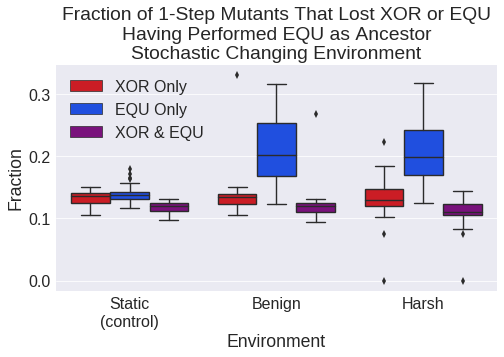
\includegraphics[width=0.75\columnwidth]{figures/CE/CSE_frac_1step__filtered__box.png}
% 	\caption{\textbf{A survey of the single-step mutational neighborhood} in the stochastic changing environment around organisms that performed the fluctuating task. Again, in the static and harsh treatments, values are comparable to the cyclic changing environment . However, in the benign treatment, the mean for the loss of the fluctuating task (\texttt{EQU}) was slightly higher in the stochastic treatment (Mdn = 0.2) than the cyclic (Mdn = 0.17), though the effect is barely statistically significant (Wilcoxon Rank-Sum Test: Z = -2.4, p = 0.015). This result is consistent with stochastic environmental change being equivalently effective at moving organisms to areas of the fitness landscape where they can more easily switch task expression.%
% 	}\label{fig:CSE_single_step}
% 	\end{figure}

% In contrast, we observed a very slight, but statistically significant increase in the fraction of 1-step mutants that lost \texttt{EQU} in the stochastic treatment versus the cyclic (Wilcoxon Rank-Sum Test: Z = -2.4, p = 0.015). This effect was matched by a slight increase in the fraction of 2-step mutants that regained \texttt{EQU} in the benign stochastic treatment vs cyclic (Wilcoxon Rank-Sum Test: Z = -18.42, p $<<$ 0.0001). This result suggests that in stochastic changing environments, benign environments might possibly perform better than harsh environments for promoting evolvability. However, because the effect sizes were so small, we cannot conclusively find that stochastic environments performing any differently than cyclic at promoting evolvbility.

% %=[FIGURES - 2-step]
% 	\begin{figure}[!h] %% FIGURE 11
% 	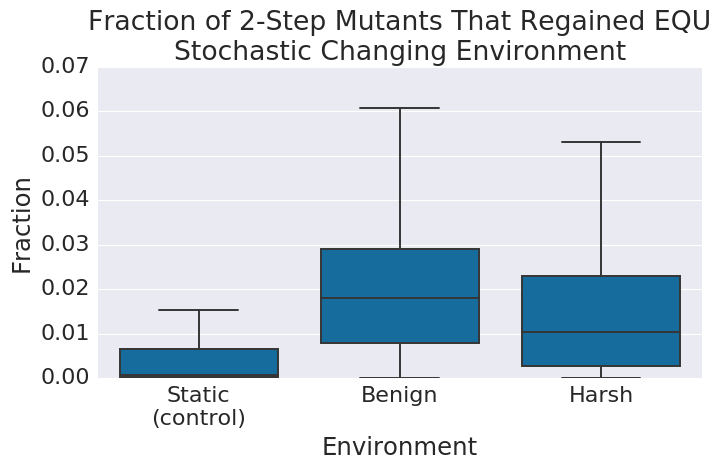
\includegraphics[width=0.75\columnwidth]{figures/CE/CSE_frac_2step__box.png}
% 	\caption{\textbf{A survey of the two-step mutational neighborhood} in the stochastic changing environment of the organisms that lost \texttt{EQU} function in the one-step survey. We found that the fraction of organisms regaining the fluctuating task (EQU) from a single additional mutation in the harsh treatment (Mdn = 0.013) were reduced compared to the cyclic harsh treatment (Mdn = 0.01) (Wilcoxon Rank-Sum Test: Z = 12.75, p $<<$ 0.0001) The opposite, however, was true of the Benign treatments. As in Fig~\ref{fig:CSE_single_step}, we find that stochastic outperforms cyclic (Wilcoxon Rank-Sum Test: Z = -18.43, p $<<$ 0.0001) This result confirms that the harsh stochastic environment is probably less effective than the cyclic harsh at promoting evolvability, but that the opposite may be true for a benign environment.
% 	}\label{fig:CSE_two_step}
% 	\end{figure}

% %=discussion of function vs vestigial
% Few differences between the cyclic and stochastic treatments also appeared in the number of functional and vestigial sites. Both the numbers of functional and vestigial sites in the stochastic environment were similar to those in the cyclic environment. In the stochastic harsh treatment, there was a small, but significant reduction in the number of XOR+EQU overlapping functional sites (Mdn = 14) as compared to the cyclic treatment (Mdn = 16) . (Fig~\ref{fig:CSE_func_vestigial}) 

% %=[FIGURE - func vestigial sites]
% 	\begin{figure}[!h]
% 	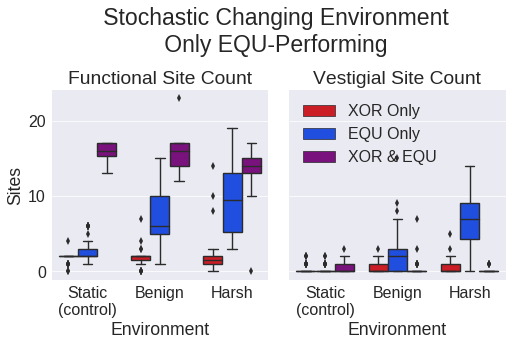
\includegraphics[width=0.75\columnwidth]{figures/CE/CSE_func_vest__filtered__box.png}
% 	\caption{\textbf{Number of functional and vestigial sites by treatment} in a stochastic changing environment. The vestigial site counts for \texttt{EQU}-only performing organisms remain comparable to the cyclic environment (Wilcoxon Rank-Sum Z = 0.46, 1.45, and -1.10, p = 0.6, 0.14, and 0.2). The functional sites were also comparable, however, there was a slight, but statistically significant decrease in the number of \texttt{XOR} \& \texttt{EQU} overlapping sites in the stochastic vs cyclic environments (Wilcoxon Rank-Sum Test: Z = -3.05, p$<$0.01).
% 	}
% 	\label{fig:CSE_func_vestigial} %% FIGURE 9
% 	\end{figure}

% %=hypothesyze these effect driven by variance in timespans
% %We hypothesize that these effects were driven by the inconsistent time spans between the population experiencing a given environmental condition in the stochastic treatments. Especially long time spans without a reward for a task, even if rare, could allow vestigial sites to drift away, thus pushing subsequent evolution closer to the control treatment. However, due to the rarity of such events, the effects of drift would be relatively limited.
% Together, from these measures, we conclude that stochastic environments exert similar evolutionary pressure to move toward regions of the mutational landscape that are more congenial to neutral phenotypic exploration and evolvability. However, the combination of the slight improvements in benign stochastic environments, matched by slight decreases in effectiveness in harsh stochastic environments, suggests that the periodicity of the cyclic environment provides a slight advantage to adapting to harsh environments. In the benign environments, however, the stochastic nature may be less of a disadvantage. We hypothesize that this dynamic may be due to the randomly-occurring environmental changes either occurring too rapidly for a response to selection, or too slowly, such that drift may cause the information contained in vestigial sites to mutate away. While the environment, on average, experiences as many changes as in the cyclic experiment, the distribution of the length of those environment periods may be very different. We conclude that our stochastic changing environment is not more effective than a cyclic changing environment, and under harsh conditions, may actually be slightly worse for promoting the evolution of evolvability.

% %@CAO - If you want to talk about how to further explore this idea, you would probably do a range of runs with different cycle periods and show that the one we're using is somehow optimal. It might be that if we compared to a non-optimal cycle time, the stochastic would do better since it would sometimes bring changes into a more optimal range
% %@RCK - One of my appendices recounts the runs we did to arrive at the 1000 update cycle time, so that wouldn't be a bad foundation for a comparison.

\subsection*{Stage 2 - Long-Term Evolvability}
\todo[inline]{Redo figures to not say "Simple Environment"}
\subsection*{Task Discovery}
Task discovery is an important measure of long-term evolvability in that it quantifies the ability of populations to explore and adapt to entirely new environments. We measured task discovery in each of the changing environment treatments.

\subsubsection*{Benign changing environments outperform harsh environments in task discovery}
% MJW: Why do you switch between capitalizing the words in the subsections and not in the sub-subsections?  This might be something you do consistently but I only noticed here because they're stacked right next to each other, in which case it's probably a formatting thing, but it seemed worth asking when I noticed it.
We found that once we began rewarding the \textbf{expanded task set}, populations evolving in harsh changing environments discovered many fewer tasks that those evolving in benign changing environments (Wilcoxon Rank Sum Test: Z = 2.75, p $<$ 0.01) (Fig~\ref{fig:postreward_task_discovery}). We hypothesize that this effect is due to the relative differences in the strength of selection between the harsh changing environment and the directional selection toward the \textbf{expanded task set}. 
%=[FIGURE - postreward task discovery]
	\begin{figure}[!h]
	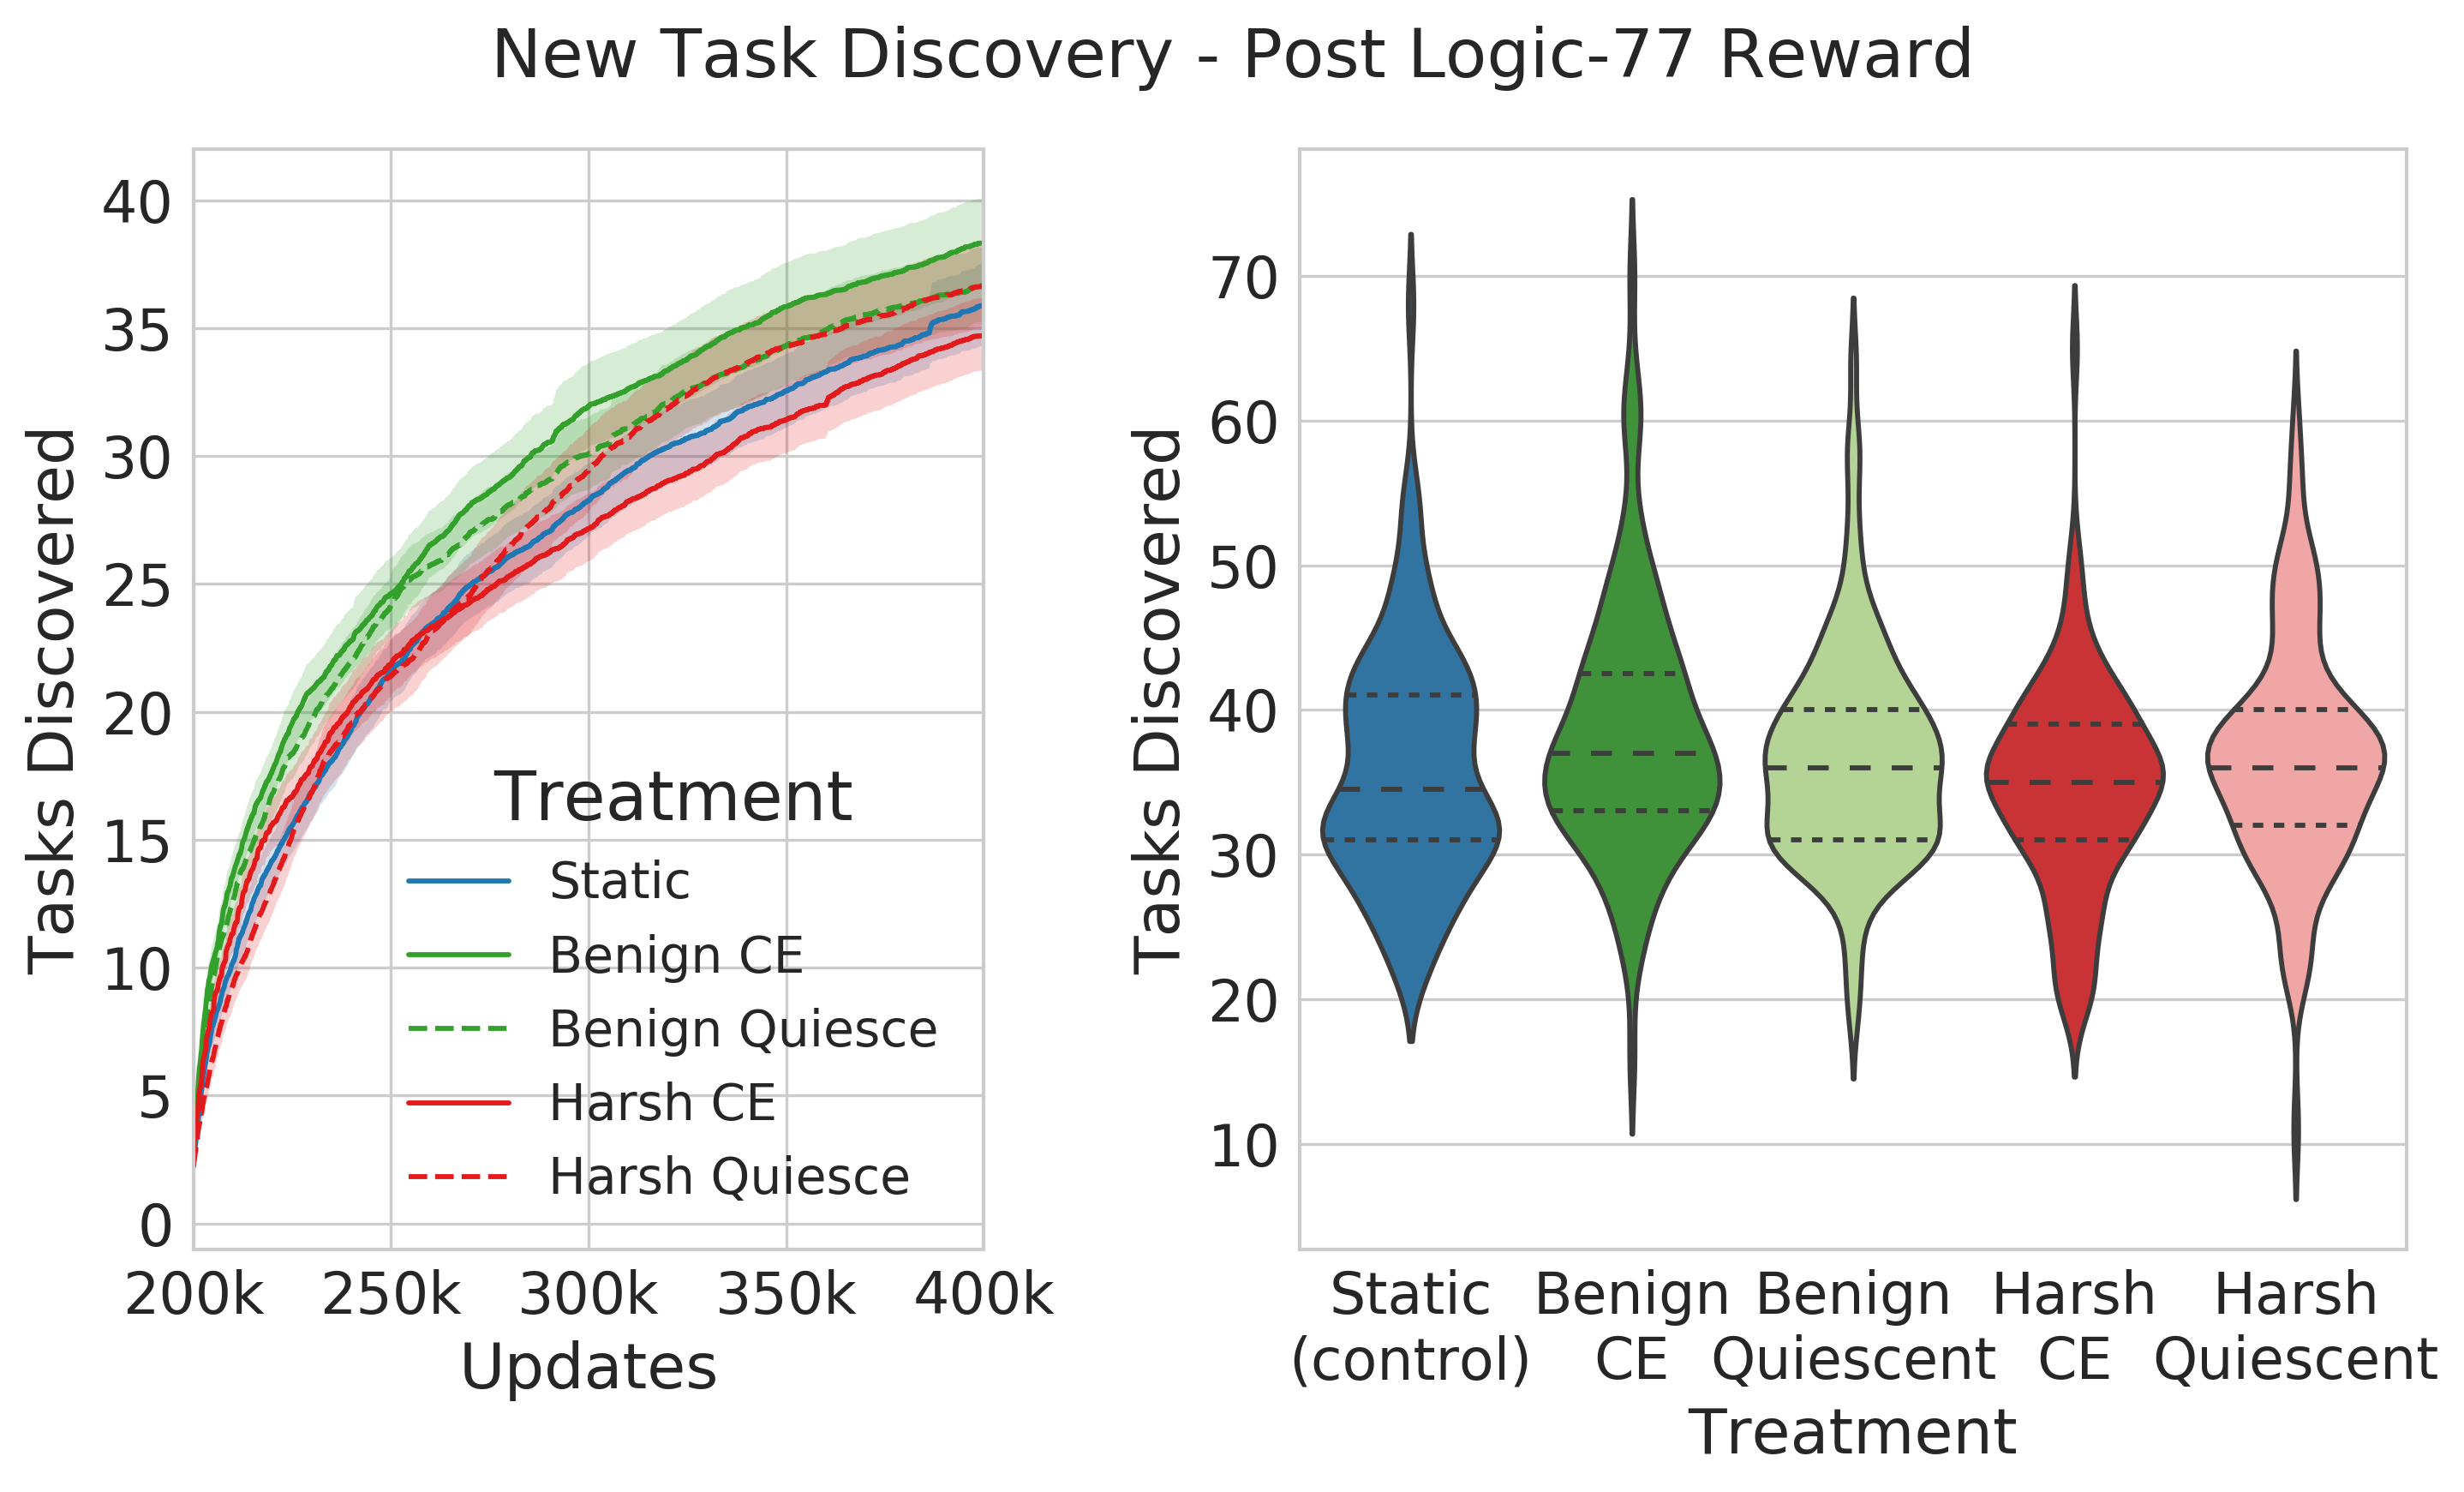
\includegraphics[width=0.95\columnwidth]{figures/LTE/lte-simple-post_reward_task_discovery.png}
	\caption{\textbf{Number of new Logic-77 tasks discovered post-reward}. The left plot shows a time-series of the number of non-ephemeral tasks discovered by populations by each treatment. The right plot shows the number of tasks discovered at the end of the experiments. While the individual values overlap their neigbors, the top and bottom-most treatments (Benign and Harsh) are significantly different from each other (Wilcoxon Rank Sum Test: Z = 2.75, p $<$ 0.01). %
	}
	\label{fig:postreward_task_discovery}
	\end{figure} 

% MJW: I am having a hard time tracking what the "relative differences" are here. The plurality implies that there are multiple, but the sentence structure seems to indicate you're comparing strength of selection in the harsh changing environment and the directional selection toward Logic-77 tasks (by which I am assuming you are referring to the selective pressure towards acquiring tasks that are always rewarded, but conceptually it's hard to compare the strength of selection [essentially a measure of s in population genetics] to directional selection [a class of selective pressure]).
%@RCK: added more detail below
In the harsh changing environments, the selective pressure to gain or lose the fluctuating tasks represents up to a $2 * 2^5$-fold bonus over the course of a single cycle, whereas the \textbf{expanded task set} can individually only offer a 1.2-fold bonus to execution speed. Thus, those organisms that promptly gain or lose a fluctuating task are more likely to survive, regardless of whether or not they have gained one of the new Logic-77 tasks. Thus pressures to gain and lose the fluctuating tasks are much stronger than the pressure to acquire new Logic-77 tasks, thereby depressing the rate at which they are found.
% MJW: I know that stats are TODO throughout this chapter, but this sentence in particular absolutely needs them, and it's the sort that would be easy to overlook so I'm flagging it. Though, to be fair, you don't necessarily need the stats if you just lay out the raw numbers -- the selective benefit towards either gaining \texttt{EQU} when it starts being rewarded or lose it when it starts being punished is X, the benefit of acquiring a Logic-77 task is Y.
%@RCK: added something to expand on the reasoning

%and keeping it comparable to the pre-phase 2 rate. 
In contrast, the benign environment experiences a weaker strength of selection for \texttt{EQU} task gain and loss, in the form of a maximum $2^5$-fold bonus directional selection pressure to gain the tasks, and no direct pressure to lose the task. Thus, when compared to the harsh treatments, the fraction of the total selective pressure for gaining new expanded tasks is greater in the benign treatment. This increased pressure, plus the benefit of an increased exploration rate conveyed by the benign changing environment, result in a higher overall task discovery rates.

%\subsubsection*{HarshQuiescent treatment outperforms BenignQuiescent treatment in task discovery.}
Interestingly, in the harsh quiescent treatment (HarshQuiescent) beginning in stage 2, we saw that task exploration recovered and achieved a comparable level to the control (Wilcoxon Rank Sum Test: Z = -0.91, p = 0.37). What could account for this recovery? 

One possibility is that the introduction of the new tasks provided sufficient selective pressure to cause the increase in the discovery rate. In this case, we would expect to see a similar increase in task exploration in the harsh changing environment treatment (HarshCE). 

Another possibility is that the alternating environment in the first part of the experiment created a diversity disadvantage in populations in those treatments. If this were the case, we would expect HarshQuiescent's task discovery to initially grow more slowly than the control, which would have suffered from no such disadvantage. Then, as diversity recovered, we would expect to see task discovery grow at comparable rates.

Finally, there is the possibility is that the alternating selection regime was directly responsible for depressing task exploration. In this case, once we stopped alternating task rewards, we would expect to see a significant difference in task discovery rates between the HarshQuiescent and HarshCE treatments. 

Indeed, we found that the the HarshQuiescent treatment has a much higher task discovery rate than the HarshCE treatment. This is inconsistent with the hypothesis that the task rewards alone account for the recovery of the HarshQuiescent. Instead, this result is consistent with the possibility of a direct negative effect from the continuing alternating selection. We also found that there was a lag in task discovery compared to the control. This suggests that there was, at least initially, some population-level disadvantage occurring in the HarshQuiescent populations. We also observed that after the initially slow recovery phase, the quiescent treatment rapidly increased its task discovery rate, and exceeded that of the control. This is consistent with a recovery of diversity, plus, potentially some lingering architectural advantage for finding new tasks.
% MJW: This is a really key finding of this chapter. I feel you could highlight this more. One writing strategy that Rich employs a lot that I find particularly effective is to structure something along the lines of "Here is a fact (either from our observation or from the literature). What could account for this?  Possible explanation 1 would predict X. Possible explanation 2 would predict Y. Possible explanation 3 would predict Z. We find N, which is inconsistent with X, and is more likely to be a result of Y than of Z, so we conclude that possible explanation 1 is not driving our results/this observation, and that possible explanation 2 is more likely than possible explanation 3". Not saying you have three possible explanations here, just a general sort of approach to that way of writing a combined results and discussion section.
%@RCK: Added more exposition along those lines.

% %\subsubsection*{BenignCE treatment outperforms BenignQuiescent treatment in task discovery.}
% %=disentangling direct effects from architectural byproducts
% Also of interest
% % MJW: Careful. It's one thing to call a result interesting; it's another to make a claim about how relatively interesting different findings are as if that is objectively measurable, rather than a personal decision.
% %@RCK: removed comparison
% is a small difference in task discovery rates between the benign environment populations BenignCE and BenignQuiescent. Once the expanded task rewards are introduced, the BenignCE populations continue to be subject to a benign changing environment, whereas the BenignQuiescent populations are only subject to directional selection toward the evolution of the original and expanded tasks. The task discovery rate for the BenignCE populations (Mdn = 37.0, CI 95\% [36.0, 38.0]) are slightly higher than for BenignQuiescent (Mdn = 36.0, CI 95\% [34.0, 38.0]), but the effect is not statistically significant (Wilcoxon Rank Sum Test: Z = 1.39, p = 0.16). This treatment, however, still performs better than the control treatment (Mdn = 34.5, CI 95\% [32.0, 38.0]), though, again, this effect is not statistically significant. What could account for this reversal of the pattern observed between HarshCE and HarshQuiescent?

% %One possibility is that the difference in selective pressures is sufficient to create a reversal. In this case, we would predict 

% One possibility is that some population-level diversity advantage is being conveyed by the activity of the benign changing environment. In this case, we would expect the BenignQuiescent task discovery rates to initially closely track that of the BenignCE treatments, and then as diversity equalized, to drop down to rates comparable to the control.

% Another possibility is that the benign changing environment is directly promoting task exploration. In this case, we would expect to see a significant difference in task discovery rates between the BenignCE and BenignQuiescent treatments.

% We observe that following the introduction of the \textbf{expanded task set}, the BenignQuiescent treatment task rates quickly depart from the BenignCE task discovery rates. This result is inconsistent with the hypothesis of a population diversity advantage. If anything, task discovery levels lag behind the control treatment. Thus, we find that it is most likely that the benign changing environment is directly promoting task discovery, though the mechanism of this promotion remains unclear.  

%Thus, this result suggests that there may be architectural features conferred by evolution in the changing environment that are helpful for long-term evolvability, even after the environmental changes have stopped, and that this effect is distinct from the direct effects of the changing direction of selection. %Further research is needed to fully untangle these effects.
%\todo[inline]{convert the Mdn and WRST stuff into a goddamned table ffs}
\subsubsection*{Harsh changing environments drive populations across the mutational landscape}
%=[FIGURE - overall task discovery]
	\begin{figure}[!h]
	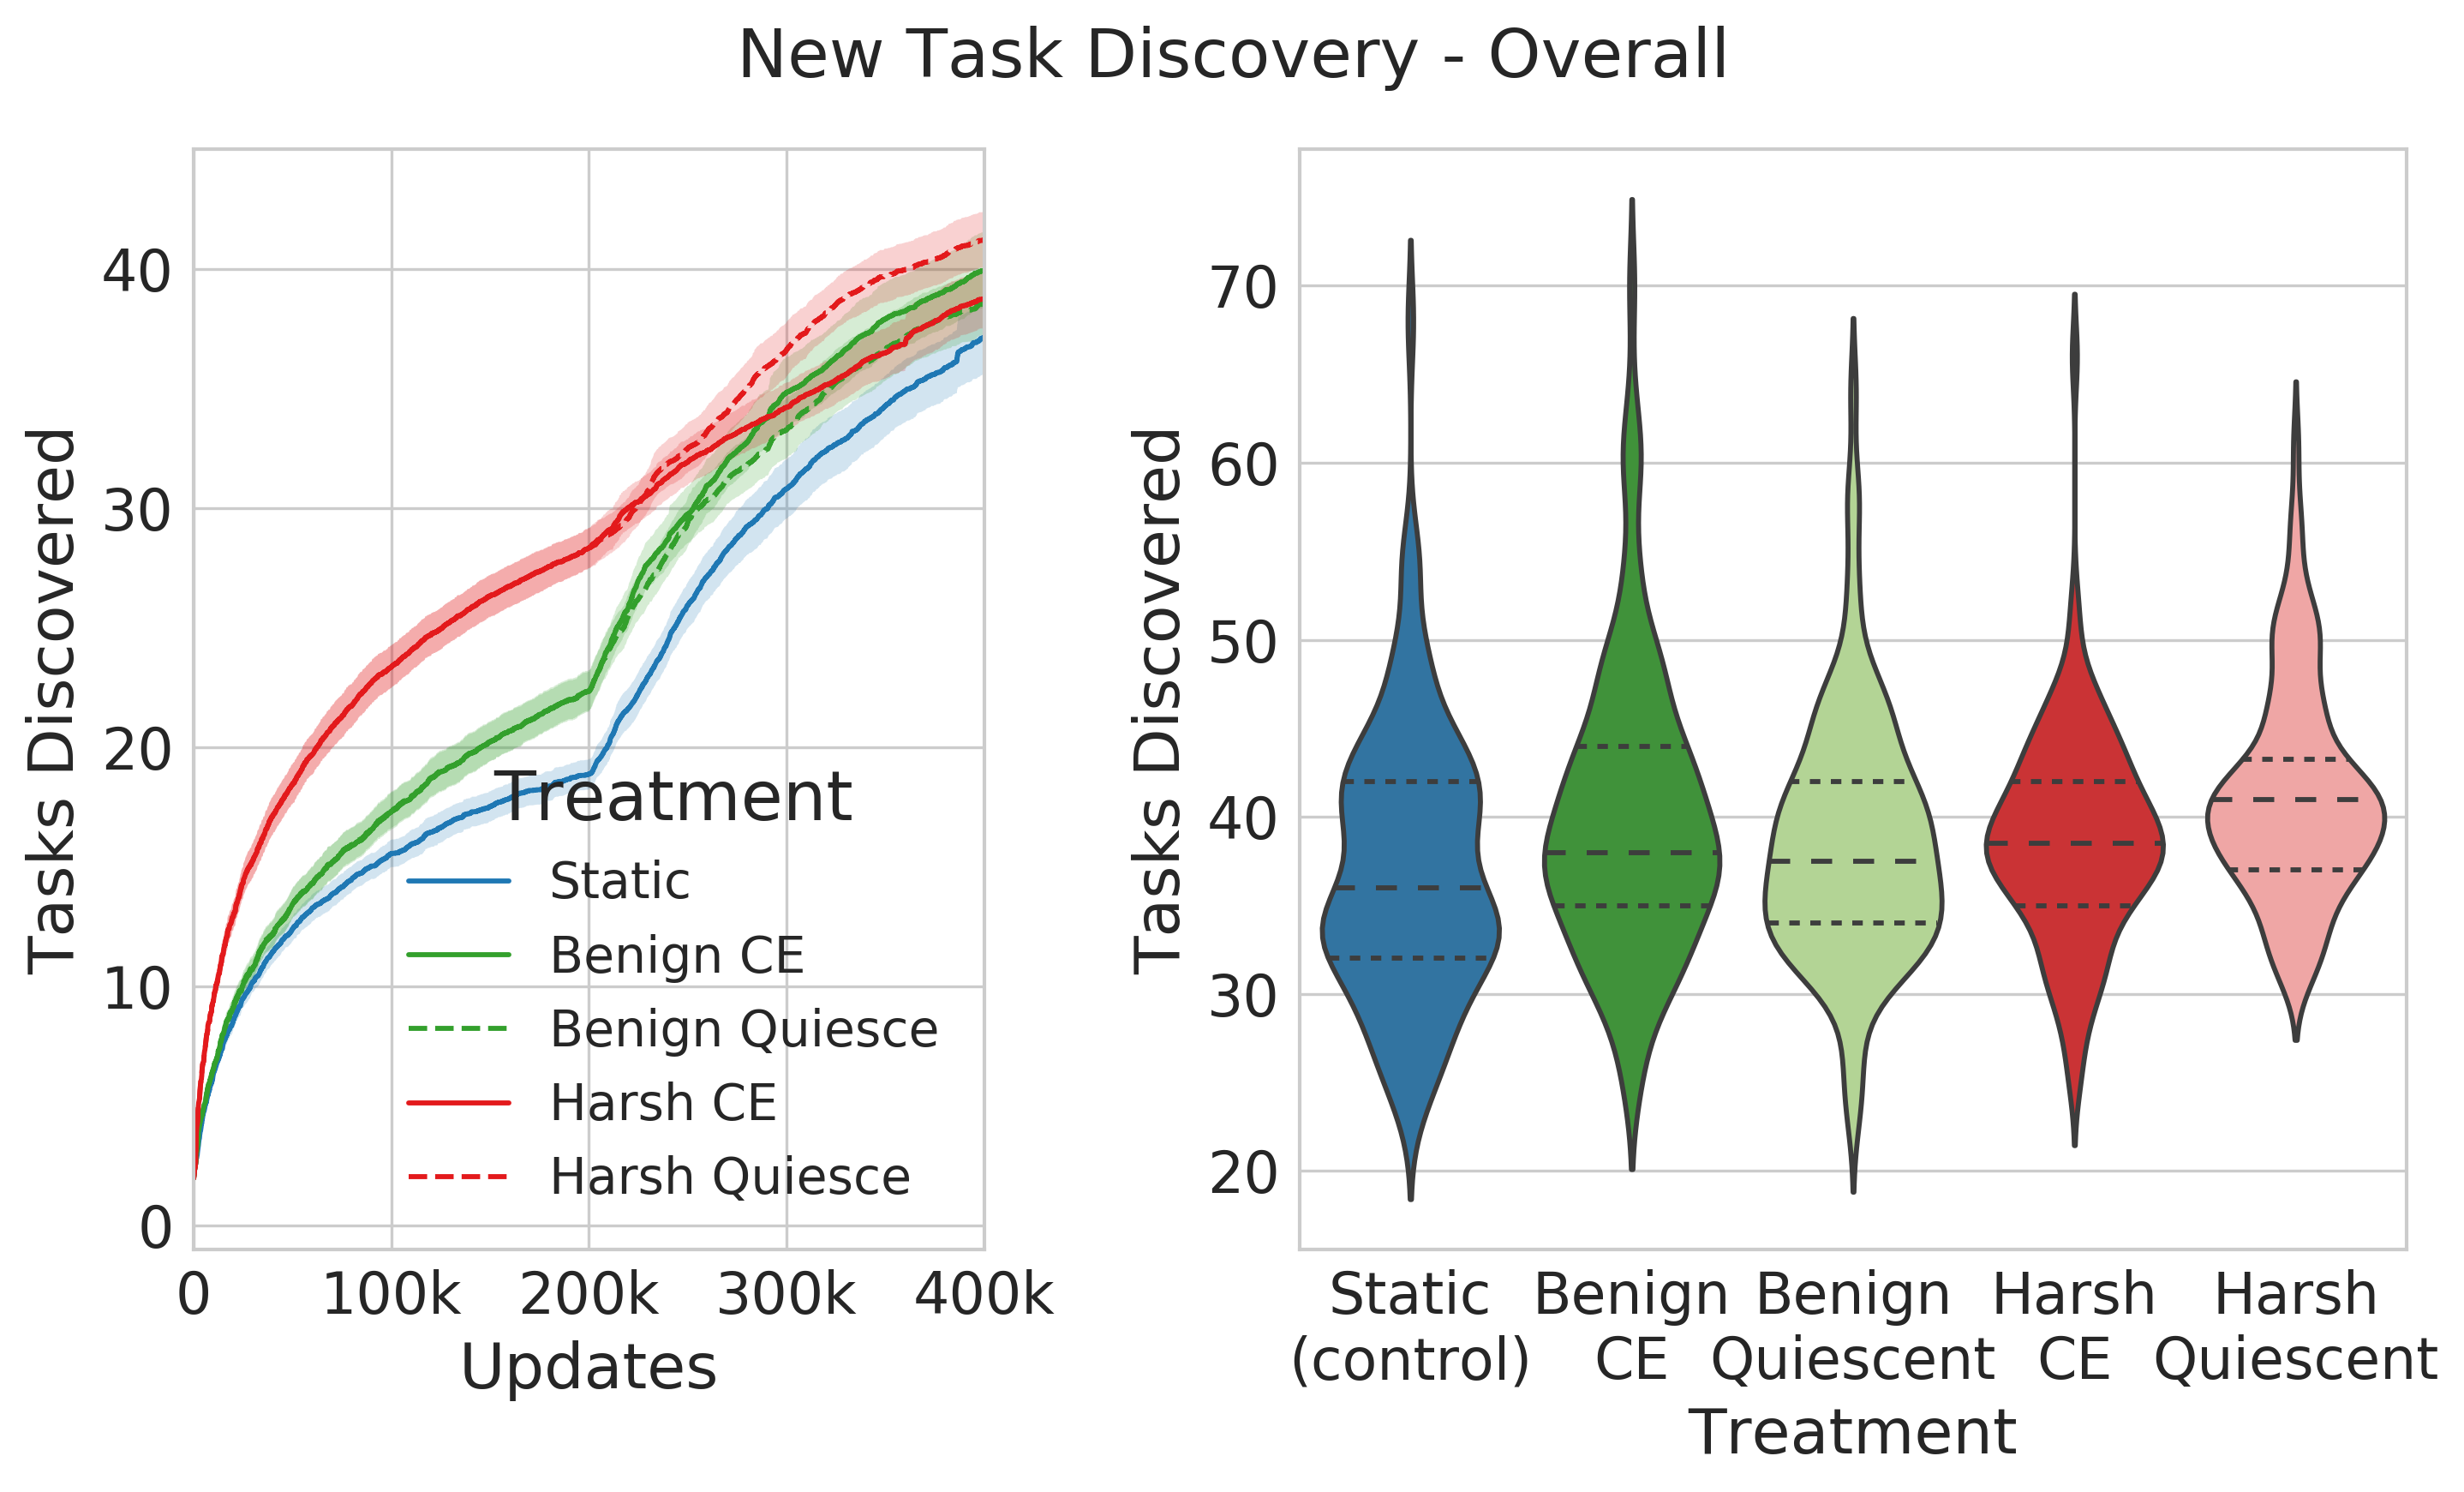
\includegraphics[width=0.95\columnwidth]{figures/LTE/lte-simple-overall_task_discovery.png}
	\caption{\textbf{Number of new Logic-77 tasks discovered over the whole experiment}. The left plot shows a time-series of all new tasks discovered over the course of the entire run, including non-rewarded Logic-77 tasks. The right-hand plot shows the final count at the end of the run. Before we introduce rewards for performing Logic-77 tasks, the harsh changing environment discovers far more new tasks (Mdn = 28.0, CI 95\% [27.0, 30.0]) than either of the other treatments (Mdn = 22.0, CI 95\% [22.0, 23.0]) (Wilcoxon Rank Sum Test: Z = 8.61, p $<<$ 0.001). This occurs despite no reward being given for performing the Logic-77 tasks in the first part of the experiment. %
	}
	\label{fig:simple-overall_task_discovery}
	\end{figure}

%=choice of CE has dramatic effects - forced march
In the first part of the experiments, despite the \textbf{expanded task set} not being rewarded, both changing-environment treatments (BenignCE and HarshCE) discovered more new tasks than the control (Wilcoxon Rank Sum Test: Z = -5.75 and -11.15 respectively, p $<<$ 0.001). The harsh treatment in particular discovered substantially and significantly more \textbf{expanded task set} tasks than either the benign treatment (Wilcoxon Rank Sum Test: Z = -8.0, p $<<$ 0.001) or the control, despite these tasks not being rewarded (Fig~\ref{fig:simple-overall_task_discovery}). We speculate that this effect may be due to the large phylogenetic depth of the harsh-evolved populations, where the repeated bottlenecks drive the populations along a kind of forced march across the mutational landscape. However, as the experiment proceeds, and Logic-77 task rewards are introduced, this effect disappears, and task discovery rates converge (Kruskal-Wallis: H(2) = 6.97, p = 0.03).


%=post-reward exploration - strength of selection differences
% Despite the initial success of the harsh-evolved populations' random walk across the fitness landscape, once selection for the Logic-77 tasks is engaged at the start of phase 2, the benign and control treatments out-perform the harsh-evolved populations in task discovery. In particular, those populations where the harsh changing environment continues, significantly under-perform in task exploration as compared to the benign-evolved populations, and are comparable to the control rate. (Fig~\ref{fig:postreward_task_discovery}). 
% (Fig~\ref{fig:composite_task_discovery} lower left)







\subsection*{Task Performance}
In addition to task discovery, task performance is another important measure of long-term evolvability, in that it quantifies exploitation and fixation of traits that are beneficial in new environments. We measured task performance in each of the changing environment treatments.

\subsubsection*{Benign changing environments outperform harsh environments in task performance}

	%=[FIGURE - postreward task performance]
	\begin{figure}[!h]
	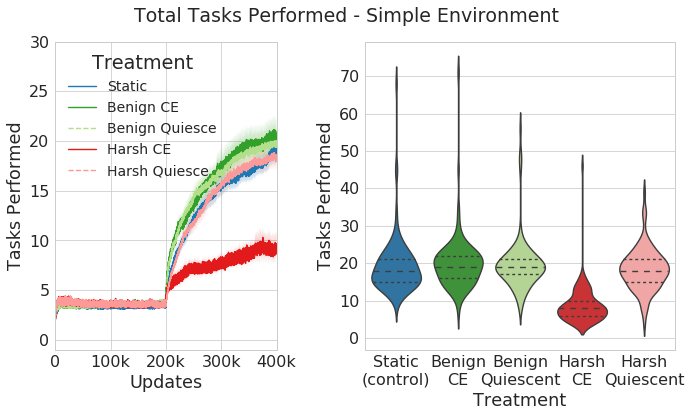
\includegraphics[width=0.95\columnwidth]{figures/LTE/lte-simple-task_performance.png}
	\caption{\textbf{Number of distinct tasks performed}. The left plot shows a time-series of the number of distinct tasks performed by the treatment populations over time. The right-had plot shows the number of tasks performed at the end of the experiments. The harsh changing environment treatment performs substantially and significantly fewer tasks than any of the benign or control treatments (Wilcoxon Rank Sum Test: Z = -11.22 and -11.15 respectively, p $<<$ 0.001). The benign treatments perform best, but the differences are not statistically significant from the control (Kruskal-Wallis: H(2) = 2.76, p = 0.25). %
	}
	\label{fig:lte-simple-task_performance}
	\end{figure}  


Similar to task discovery, populations evolving in harsh changing environments performed far fewer distinct tasks than either the control, or either benign populations (Wilcoxon Rank Sum Test: Simple: Z = -11.22 and -11.15 respectively) (Fig~\ref{fig:lte-simple-task_performance}). While both the BenignCE and BenignQuiescent
% MJW: Inconsistent capitalization w/r/t the previous sentence.
%@RCK: fixed
populations seemed to outperform the control, 
%this effect was only statistically significant in the rich environment (Wilcoxon Rank Sum Test: Z = 2.42 and 2.37 respectively, p $<$ 0.05). In the minimal environment, 
the differences were not statistically significant (Kruskal-Wallis: H(2) = 2.76, p = 0.25).


% %\subsubsection*{Benign changing environments outperform harsh environments in task discovery and task performance}
% Similar to the results of the simple environments, Benign-evolved populations out-perform Harsh-evolving
% % MJW: You're inconsistent on whether the populations are evolved or evolving. Or, well, you're comparing this at the end of the benign environment to things not at the end of the harsh environment, which means you're got time as a confounding factor.
% populations in complex changing environments 
% %in measures of Task Performance (Fig~\ref{fig:complex-task_performance}) and Task Discovery 
% (Fig~\ref{fig:complex-task_discovery}). Again, this result suggests that, despite the differences in genome composition and environmental complexity, Benign changing environments, with their gentler selective pressures, or possibly with more intact chunks of undisturbed functionality in their genomes, leave more room for populations to acquire new tasks without the risk of harsh punishments. 
% %MAYBE NOT?
% %Both types of Benign-evolved environment appear to out-perform the control, but the effect is not statistically significant.


% % below is speculative!!!
% Interestingly, in the rich environments, the HarshQuiescent treatments %that were initially evolved in a harsh changing environment and then change ceased upon introduction of Logic-77 rewards (Harsh Quiescent)
% % MJW: "change ceased upon introduction..."?  I don't understand. I'm unsure whether change ceased is an adjective of the populations, or if changed ceased (noun - verb) when you moved them to a different environment.
% %@RCK: fixed
% seemed to out-perform all other environment types in task performance, though the differences between HarshQuiescent and both benign treatments are only barely statistically significant (Wilcoxon Rank Sum Test: Control Z = 4.33, HarshCE Z = -9.3, p $<$ 0.001; BenignCE Z = 2.25, Benign Quiesce Z = 1.96, p $<$ 0.05). We speculate that this effect may be due to a lingering architectural effect of evolving in harsh changing environments. For example, because task length increases in changing environments, these tasks are more likely to experience mutations that could change their phenotype in a variety of ways. Thus, once the pressure to limit diversity is released, the population would be much more likely to produce a large amount of population variation in a short time. Thus, we would expect to see a significant increase in measures of task performance, but might also expect to see a relatively lower number of task being performed by the entire population.
% % MJW: I suggest that if you're going to speculate, speculate. In other words, either expand this section with one or more examples of what sort of architectural effect you mean, or cut this sentence.
% %@RCK: added moar speculation.
% Further research is needed to identify the mechanisms responsible for this effect.


\section*{Conclusion}

%=direction of selection drives exploration and gathers history
In cyclic changing environments, the direction of selection shifts frequently, and periodically drives populations to not only explore new regions of the genetic landscape, but also to carry with them vestigial genetic information about previous environmental conditions. Thus, the resulting populations are not only adapted to the current environment, but also to the meta-environment of cyclic change. Because of their evolutionary history, the genomes contain vestigial fragments of genetic material that were adapted to prior environments. As this exploration proceeds, mutations accumulate in the population, each creating a link to a new region of the mutational landscape. As these links accumulate, they form a reservoir of mobility for the population to quickly shift to new phenotypes as dictated by current selective conditions. In this way, the accumulation of vestigial or pseudogene-like regions acts as an indirect adaptation to the larger pattern of changing selective forces. 
%@CAO - This argument clearly implies that evolvability is not actually selected for. It's merely a by-product of how changing environments naturally alter genomes by creating genetic reservoirs. I feel like this is a point that we might want to hilight further.
%@RCK - agree. done, below.

%=by constrast static environments don't
By contrast, in static (non-changing) environments, the majority of neutral mutations do not connect to as many phenotypically-interesting regions of genotype-space. There are far fewer pseudogene-like regions available that could regain functionality should conditions change. Thus, populations evolved in static environments are less evolvable in the short-term.

These results suggest, therefore, that architectural features that help with short-term evolvability are more likely the result of repeated hitchhiking on adaptive mutants. In particular, we observed that much of the task-loss associated with the harsh changing environment could be attributed to increasing task length which is a result of the continuous addition of new mutations activating and deactivating the task. Despite this correlation, however, we observed a potential difference in robustness between the \texttt{XOR} and \texttt{EQU} tasks, which suggest that a kind of anti-robustness may also be selected for as a result of the changing environments.

% %=SCE not more effective
% Surprisingly, stochastically changing environments are not more effective at exploration
% % @CAO: Are they really?  We've shown that they produce new phenotypes less often, but that's a very limited definition of exploration. However, it's the one that we need to stick to.
% % @CAO: That said (and this argument goes to static environments too), if we claim that stochastic environments produce new phenotypes less frequently we can argue WHY we hypothesize that they'll be less effective at exploration. In thinking about it, it feels like we should use these as ancestors for an entirely new environmental shift. If we show that the organisms previously experiencing a cyclically changing environment do better with the new environment THEN we have strong evidence that stochastically changing environments are less effective at exploration.
% than cyclic changing environments, even if, on average, the amount of time spent in each environment was equal. We hypothesize that this result is because of more opportunity for drift to destroy the information contained in vestigial regions, as well as potentially fewer opportunities for populations to respond to selection.


\subsection*{Long-Term Evolvability}
The relationship between short and long term evolvability is non-obvious. Architectural features and selective pressures that promote repeated re-adaptation to a known set of environments may not be beneficial for the acquisition of entirely new adaptive traits. For example, harsh changing environments act to depress both fitness and population diversity, which might make these populations less effective at adaptation when introduced into a new environment.

Indeed, our experiments show that harsh changing environments, with their strong selective pressures, suppress the ability of populations to acquire new, weakly-selected traits. However, benign changing environments, with their milder set of selective pressures, are able to leverage their accumulated heritage of dormant vestigial sites to rapidly respond to selection, and acquire new tasks at a faster rate than either harsh or non-change-evolved populations. However, despite the direct negative effects of harsh changing environments, populations initially evolved in these environments are able to rapidly acquire new tasks if alternating selection is removed. This result suggests that there are important architectural features conveyed by these environments that are beneficial for new task acquisition.


\subsection*{Limitations of Cyclic Changing Environments}
%=CE can be a re-tread, but not as much as feared 
Changing environments produce a set of selective pressures that speed up exploration of genotype space, while also building reservoirs of partial functionality that may be co-opted in the evolution of more complex structures. These features make changing environments useful for both their exploratory power in natural evolution, and as practical tools in the Artificial Life toolkit.
Ultimately, however, as alluded to above, cyclic changing environments only re-tread existing phenotypic ground, and though genotypic exploration can be faster than under purely directional or stabilizing selection, the space explored remains constrained by the type of phenotypes that are selected. Despite this constraint, however, we see that, particularly under harsh conditions, a lot of novel genotypic ground may be explored, even without direct selection for novelty. 

%=better/different methods
Even so, there must exist methods of exploring genotype space that do not suffer from these limitations at all.
For example, perhaps repeated bottlenecking of populations could promote faster traversal of the fitness landscape in quasi-random directions. More ambitiously, perhaps these kinds of environments could be coupled with dynamically increasing open-ended complexity goals, or divergent selection mechanisms such as negative frequency dependence to promote the maintenance of diversity in evolving populations.

%=understanding is vital, conclusion paragraph
Understanding the mechanisms by which select environmental conditions alter fitness landscapes is vital to understanding the forces that promote evolvability and increase complexity. In particular, understanding the role of vestigial sites may help us untangle how robustness can promote evolvability. Are these vestigial sites merely inactive remnants, reservoirs of function, or are they part of a complex compensatory framework supporting and buffering the expression of the phenotype? Or all of these things? Changing environments provide one view into these dynamics, but we must explore further to find other mechanisms for exploring and exploiting genotype space.

\section*{Acknowledgments}
We would like to thank Alex Lalejini for helpful discussions and comments about the relationship between phenotypic plasticity and contingency loci, Josh Nahum for discussions of experiments in changing environments, and Emily Dolson, Brian Goldman, and Anya Vostinar for their comments on early manuscript drafts.
This material is based in part upon work supported by the National Science Foundation under Cooperative Agreement No. DBI-0939454 to CO and a Graduate Research Fellowship to RCK. Any opinions, findings, and conclusions or recommendations expressed in this material are those of the author(s) and do not necessarily reflect the views of the National Science Foundation.

%\bibliographystyle{apalike}
\bibliography{changing_env}


\end{document}